\documentclass[letterpaper]{article} % DO NOT CHANGE THIS
\usepackage[preprint]{aaai2027}  % DO NOT CHANGE THIS
% The serif, sans-serif, and monospaced fonts are loaded automatically by
% aaai2027.sty (newtxtext, helvet, courier). DO NOT add \usepackage{times},
% \usepackage{helvet}, \usepackage{courier}, or any other font package.
\usepackage[hyphens]{url}  % DO NOT CHANGE THIS
\usepackage{graphicx} % DO NOT CHANGE THIS
\urlstyle{rm} % DO NOT CHANGE THIS
\def\UrlFont{\rm}  % DO NOT CHANGE THIS
\usepackage{natbib}  % DO NOT CHANGE THIS AND DO NOT ADD ANY OPTIONS TO IT
\usepackage{caption} % DO NOT CHANGE THIS AND DO NOT ADD ANY OPTIONS TO IT
\frenchspacing  % DO NOT CHANGE THIS
%
% These are recommended to typeset algorithms but not required. See the subsubsection on algorithms. Remove them if you don't have algorithms in your paper.
\usepackage{algorithm}
\usepackage{algorithmic}
\usepackage{dblfloatfix}
\usepackage{amsmath}
%
% These are recommended to typeset listings but not required. See the subsubsection on listing. Remove this block if you don't have listings in your paper.
\usepackage{newfloat}
\usepackage{listings}
\DeclareCaptionStyle{ruled}{labelfont=normalfont,labelsep=colon,strut=off} % DO NOT CHANGE THIS
\lstset{%
	basicstyle={\footnotesize\ttfamily},% footnotesize acceptable for monospace
	numbers=left,numberstyle=\footnotesize,xleftmargin=2em,% show line numbers, remove this entire line if you don't want the numbers.
	aboveskip=0pt,belowskip=0pt,%
	showstringspaces=false,tabsize=2,breaklines=true}
\floatstyle{ruled}
\newfloat{listing}{tb}{lst}{}
\floatname{listing}{Listing}


% \newcommand{\liu}[1]{\textcolor{red}{Liu: #1}}
% \newcommand{\wang}[1]{\textcolor{blue}{Wang: #1}}
%
% Recommended for better-looking tables
\usepackage{booktabs}
\usepackage{amsfonts} % 
%
% Keep the \pdfinfo as shown here. There's no need
% for you to add the /Title and /Author tags.
\pdfinfo{
/TemplateVersion (2027.1)
}

% DISALLOWED PACKAGES
% \usepackage{authblk} -- This package is specifically forbidden
% \usepackage{balance} -- This package is specifically forbidden
% \usepackage{CJK} -- This package is specifically forbidden
% \usepackage{float} -- This package is specifically forbidden
% \usepackage{flushend} -- This package is specifically forbidden
% \usepackage{fullpage} -- This package is specifically forbidden
% \usepackage{geometry} -- This package is specifically forbidden
% \usepackage{hyperref} -- This package is specifically forbidden
% \usepackage{navigator} -- This package is specifically forbidden
% (or any other package that embeds links such as navigator or hyperref)
% \usepackage{indentfirst} -- This package is specifically forbidden
% \usepackage{layout} -- This package is specifically forbidden
% \usepackage{multicol} -- This package is specifically forbidden
% \usepackage{nameref} -- This package is specifically forbidden
% \usepackage{savetrees} -- This package is specifically forbidden
% \usepackage{setspace} -- This package is specifically forbidden
% \usepackage{stfloats} -- This package is specifically forbidden
% \usepackage{tabu} -- This package is specifically forbidden
% \usepackage{titlesec} -- This package is specifically forbidden
% \usepackage{tocbibind} -- This package is specifically forbidden
% \usepackage{ulem} -- This package is specifically forbidden
% \usepackage{wrapfig} -- This package is specifically forbidden
% DISALLOWED COMMANDS
% \nocopyright -- Your paper will not be published if you use this command
% \addtolength -- This command may not be used
% \balance -- This command may not be used
% \baselinestretch -- Your paper will not be published if you use this command
% \clearpage -- No page breaks of any kind may be used for the final version of your paper
% \columnsep -- This command may not be used
% \newpage -- No page breaks of any kind may be used for the final version of your paper
% \pagebreak -- No page breaks of any kind may be used for the final version of your paper
% \pagestyle -- This command may not be used
% \tiny -- This is not an acceptable font size.
% \vspace{- -- No negative value may be used in proximity of a caption, figure, table, section, subsection, subsubsection, or reference
% \vskip{- -- No negative value may be used to alter spacing above or below a caption, figure, table, section, subsection, subsubsection, or reference

\setcounter{secnumdepth}{2} %May be changed to 1 or 2 if section numbers are desired.

% The file aaai2027.sty is the style file for AAAI Press
% proceedings, working notes, and technical reports.
%

% Title

% Your title must be in mixed case, not sentence case.
% That means all verbs (including short verbs like be, is, using,and go),
% nouns, adverbs, adjectives should be capitalized, including both words in hyphenated terms, while
% articles, conjunctions, and prepositions are lower case unless they
% directly follow a colon or long dash
\title{Beyond Task-Only Matching: Personalized Skill Routing with Counterfactual Evaluation}
\author{
    %Authors
    % All authors must be in the same font size and format.
    Written by AAAI Press Staff\textsuperscript{\rm 1}\thanks{With help from the AAAI Publications Committee.}\\
    AAAI Style Contributions by Peter Patel Schneider,
    Sunil Issar,\\
    J. Scott Penberthy,
    George Ferguson,
    Hans Guesgen,
    Francisco Cruz\equalcontrib\corresponding,
    Marc Pujol-Gonzalez\equalcontrib\corresponding
}
\affiliations{
    %Afiliations
    \textsuperscript{\rm 1}Association for the Advancement of Artificial Intelligence\\
    % If you have multiple authors and multiple affiliations
    % use superscripts in text and roman font to identify them.
    % For example,

    % Sunil Issar\textsuperscript{\rm 2},
    % J. Scott Penberthy\textsuperscript{\rm 3},
    % George Ferguson\textsuperscript{\rm 4}\corresponding,
    % Hans Guesgen\textsuperscript{\rm 5}
    % Note that the comma should be placed after the superscript

    1101 Pennsylvania Ave, NW Suite 300\\
    Washington, DC 20004 USA\\
    % email address must be in roman text type, not monospace or sans serif
    proceedings-questions@aaai.org
%
% See more examples next
}

%Example, Single Author, ->> remove \iffalse,\fi and place them surrounding AAAI title to use it
\iffalse
\title{My Publication Title --- Single Author}
\author {
    Author Name
}
\affiliations{
    Affiliation\\
    Affiliation Line 2\\
    name@example.com
}
\fi

% \iffalse
%Example, Multiple Authors, ->> remove \iffalse,\fi and place them surrounding AAAI title to use it
\title{Beyond Task-Only Matching: Personalized Skill Routing with Counterfactual Evaluation}
\author {
    % Authors
    Tianle Wang\textsuperscript{\rm 2}\equalcontrib,
    Yanghe Zou\textsuperscript{\rm 1}\equalcontrib,
    Xiang Liu\textsuperscript{\rm 1,\rm 3},
    Ziyao Huang \textsuperscript{\rm 4},
    Chenchen Fu \textsuperscript{\rm 1},
    Weiwei Wu \textsuperscript{\rm 1}
}
\affiliations {
    % Affiliations
    \textsuperscript{\rm 1}School of Computer Science and Engineering, Southeast University \\
    \textsuperscript{\rm 2}College of Software Engineering, Southeast University\\
    \textsuperscript{\rm 3}Department of Computer Science and Engineering, The Chinese University of Hong Kong\\
    \textsuperscript{\rm 4}Department of Computer Science, City University of Hong Kong\\
    
}
% \fi

\frenchspacing

\begin{document}

\maketitle

\begin{abstract}
The rapid expansion of reusable skill repositories makes skill routing a critical capability for large language model (LLM) agents. Existing methods treat routing as task-only semantic matching.
However, when users with incompatible constraints issue an identical request, this assumption conflates task relevance with skill suitability: a task-only router can select a semantically plausible skill that is unsuitable for the requesting user. 
To expose this failure mode, we formulate \textit{personalized skill routing} as profile-conditioned retrieval, in which relevance depends jointly on the task and the user profile. We first introduce a profile-counterfactual benchmark, in which the task is held fixed while changes in the user profile induce changes in the reference skill. We further construct paired counterfactual supervision and propose SkillFeed, a progressive retrieve-and-rerank framework that first establishes task--skill alignment and then learns profile-conditioned discrimination. By retrieving body-level evidence and reranking semantically similar but profile-conflicting candidates, SkillFeed identifies skills that satisfy both task requirements and user constraints. 
On SkillFeed-Bench, SkillFeed attains 75.1\% top-1 retrieval accuracy, a 23.1-point improvement over the corresponding pretrained routing baseline. Adding profile conditioning yields a 35.1-point gain on queries where user profile changes the reference skill. This contrast shows that user profiles are most consequential precisely when they change skill suitability. Our website is publicly available at \url{http://www.aiskillfeed.com}.
\end{abstract}

% \begin{abstract}
% % AAAI creates proceedings, working notes, and technical reports directly from electronic source furnished by the authors. To ensure that all papers in the publication have a uniform a\%earance, authors must adhere to the following instructions.
% % Current LLM agent skill routing systems for Large Language Model (LLM) agents treat skill recommendation as a task-only matching problem, failing to capture how user context such as budget limits, platform preferences, or expertise levels alters the correct retrieval target different users require fundamentally different skills for the exact same task.
% With the rapid growth of reusable skill repositories, selecting appropriate skill becomes increasingly challenging for large language model agents.
% Existing skill routing methods primarily formulate skill selection as a task-only matching problem, failing to account for user-specific profile.
% %Different users require fundamentally different skills for the exact same task. However, current LLM agent skill routing systems treat recommendation as a task-only matching problem, failing to capture how user contexts (such as budget limits, platform preferences, or expertise levels) alter the correct retrieval target skill.
% % Current skill routing systems for Large Language Model (LLM) agents treat skill recommendation as a task-only matching problem. They fail to capture how user contexts such as budget limits, platform preferences, or expertise levels alter the required skill for the exact same task. 
% %To address this, we first formally define personalized skill routing, a setting in which skill relevance is conditioned on both the task and the user profile. 
% To address this limitation, we first formalize \textit{personalized skill routing}, where skill relevance is jointly conditioned on the task and the user profile. 
% Secondly, we introduce SkillFeed-Bench, a personalized skill retrieval benchmark built over 228K candidate skills with 329 test instances in which the  annotated reference target varies according to personalization factors.
% %To evaluate this, we introduce SkillFeed-Bench, a personalized skill retrieval benchmark built over a repository of 228K candidate skills, comprising 329 test samples where persona changes induce ground-truth shifts. 
% Thirdly, we construct user profile-aware supervision data to fine-tune a dense retriever and a cross-encoder reranker. 
% %Furthermore, we automatically construct persona-aware supervision data to fine-tune both a dense retriever and a cross-encoder reranker, adapting them to learn relevance measures conditioned on user profiles rather than on task semantics alone.
% Based on these components, we finally develop SkillFeed, a two-stage retrieval framework that combines task dense retrieval, BM25, and user profile-aware retrieval over \texttt{SKILL.md} chunks to capture fine-grained user-specific constraints, followed by a user profile-aware cross-encoder reranker for refined skill ranking.
% %We integrate these fine-tuned components into SkillFeed, a scalable two-stage retrieval pipeline that separates broad candidate recall combining task dense retrieval, BM25, and persona dense retrieval over \texttt{SKILL.md} chunks. 
% Experiments show that our approach improves Hit@1 by 23.1\% over the  pretrained baseline. 
% Notably, when isolating the effect of user profile conditioning, the performance gains are overwhelmingly concentrated on user profile-sensitive subsets, showing a 35.1\% improvement compared to a mere 0.8\% on insensitive samples.
% This demonstrates that personalization is critical when user context determines the correct skill.
% \end{abstract}
% Uncomment the following to link to your code, datasets, an extended version or similar.
% You must keep this block between (not within) the abstract and the main body of the paper.
% Make sure that you do not de-anonymize yourself with these links.
% \begin{links}
%     \link{Code}{https://aaai.org/example/code}
%     \link{Datasets}{https://aaai.org/example/datasets}
%     \link{Extended version}{https://aaai.org/example/extended-version}
% \end{links}

\section{Introduction}
\label{sec:intro}
Large language model (LLM) agents increasingly reason, call tools, and execute multi-step workflows~\citep{yao2023react,schick2024toolformer,shen2023hugginggpt}. In these systems, \emph{skills} package reusable procedures, tool-use strategies, and execution constraints in versioned bundles with \texttt{SKILL.md} manifests~\citep{openai2026skills,zheng2026skillrouter}. As public repositories grow, an agent must route each request to the skill that best supports its intended execution, making skill routing a central retrieval problem~\citep{li2025skillflow,zheng2026skillrouter}.

% Large Language Model (LLM) agents have evolved from conversational assistants into systems that reason, 
% call tools, and execute multi-step workflows~\citep{yao2023react,schick2024toolformer,shen2023hugginggpt}.
% In these systems, reusable procedures are organized as \emph{skills}, 
% reusable versioned file bundles with \texttt{SKILL.md} manifests for modular instructions, processes, and conventions~\citep{openai2026skills,zheng2026skillrouter}.
% By reusing such skills, agents can execute recurring task patterns more efficiently for specific request~\citep{openai2026skills}.
% As public skill repositories grow, skill routing becomes necessary for selecting the appropriate skill for different requests~\citep{li2025skillflow,zheng2026skillrouter}.

% Existing skill routing methods mainly formulate this problem as task-to-skill semantic matching~\citep{zheng2026skillrouter,li2025skillflow,wang2026r3skill}.
% This formulation is effective when the task uniquely determines the target skill, but it may become insufficient when user profile changes the appropriate execution path~\citep{koren2009matrix}.
% As illustrated in Figure~\ref{fig:motivation}, the same travel-planning task is routed to a budget itinerary skill for a student and to a premium itinerary skill for a business traveler.
% The task text is identical, but the preferred skill may change with user profile attributes such as payment preference, budget, and professional background.
% This motivates personalized skill routing to incorporate user profile attributes into the routing condition to better match different user tasks.

Most existing methods cast skill routing as task-to-skill semantic matching~\citep{zheng2026skillrouter,li2025skillflow,wang2026r3skill}. This formulation assumes that the task uniquely determines the appropriate skill. In practice, however, a task describes \emph{what} a user wants to accomplish, whereas a user profile can determine \emph{how} that task should be carried out. When two users issue the same request under incompatible constraints, a task-only router may select a skill that is semantically relevant but unsuitable for one of them. For example, a workflow that relies on an unavailable platform, exceeds a budget, or assumes expertise the user does not have. As illustrated in Figure~\ref{fig:motivation}, the same travel-planning request calls for a budget itinerary skill for a student and a premium itinerary skill for a business traveler. The task is unchanged, but the appropriate skill changes with profile attributes such as budget, payment preference, platform ecosystem, and professional background.

\begin{figure}[t]
    \centering
    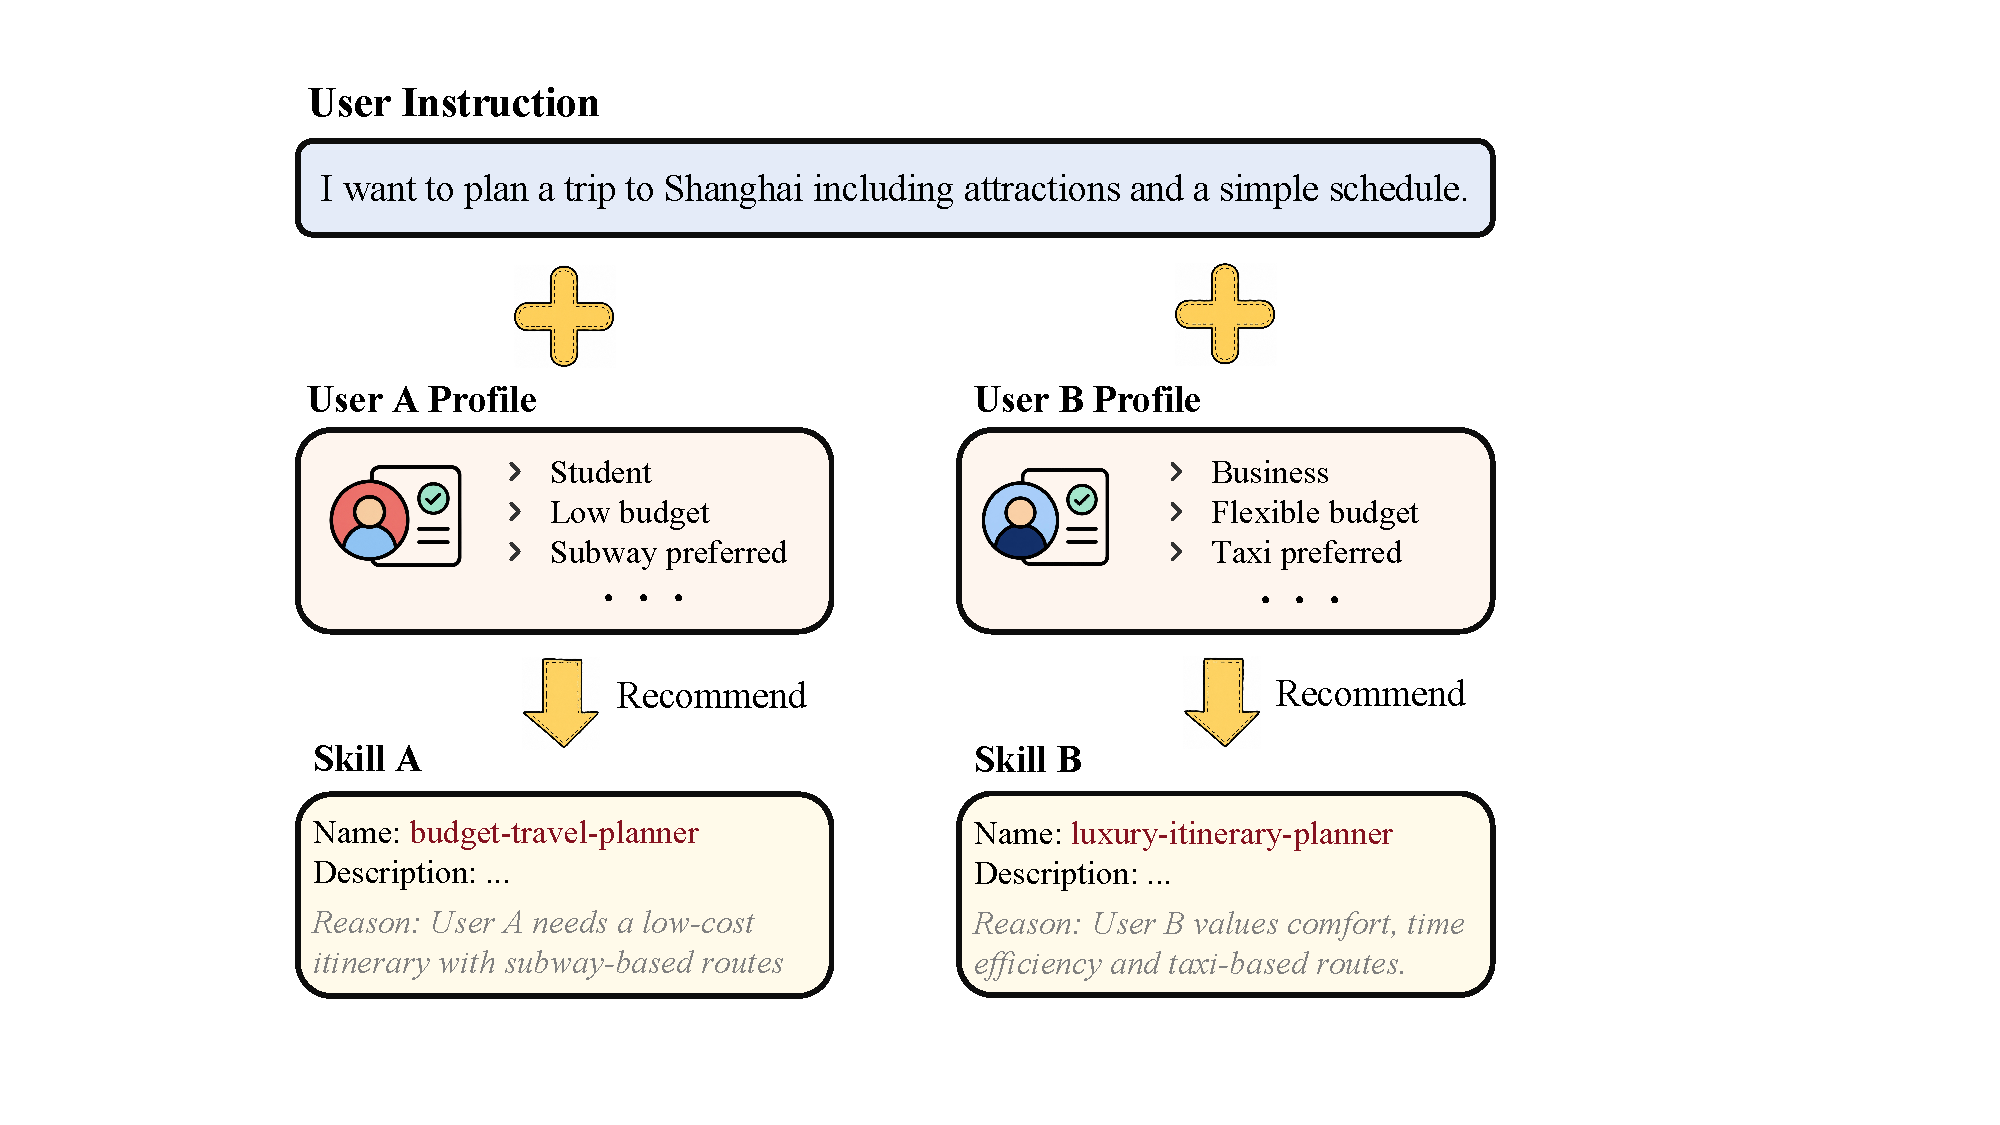
\includegraphics[width=0.84\columnwidth]{Figures/fig1.pdf}
    \caption[Example of personalized skill routing.]{Motivation example of personalized skill recommendation.
    The same task, "planning a trip to Shanghai," is routed to a budget travel planner for a student and to a luxury itinerary planner for a business traveler.
    The target skill changes with user profile.}
    \label{fig:motivation}
\end{figure}

% Prior work has introduced benchmarks for skill learning and routing, as well
% as retrieve-and-rerank systems for selecting skills from large
% repositories~\citep{li2026skillsbenchbenchmarkingagentskills,
% zheng2026skillrouter,wang2026r3skill}. However, these benchmarks and routing methods generally condition relevance on the task alone, leaving profile-dependent changes in the preferred skill largely unevaluated. We discuss these two lines of work in the Section \ref{sec:related_work}.

This failure mode cannot be established with conventional task-level evaluation. Prior benchmarks for skill learning, execution, and routing pair a request with suitable skills, while existing retrieve-and-rerank systems are trained and evaluated primarily on task--skill relevance~\citep{li2026skillsbenchbenchmarkingagentskills,zheng2026skillrouter,wang2026r3skill}. Such evaluation cannot distinguish a system that truly uses a profile from one that ignores it: when the task remains fixed, it never asks whether the predicted skill should change as the user profile changes. The resulting data also provide limited supervision for separating skills that are equally relevant to the task but conflict in their compatibility with user constraints.

% Existing skill benchmarks provide evaluation settings for skill-enabled execution and lifelong skill discovery~\citep{li2026skillsbenchbenchmarkingagentskills,zhang2026skillflowbench}.
% Other datasets focus on continual skill learning, skill generation, and repository-scale skill routing~\citep{zhong2026skilllearnbench,zhou2026skillgenbench,zheng2026skillrouter}.
% These benchmarks mainly define supervision at the task or query level, where a request is paired with suitable skills, generated skills, or compatible skill sets~\citep{wang2026r3skill}.
% user profile is not modeled as part of the ground-truth condition.
% As a result, existing benchmarks do not directly evaluate whether the same request should be routed to different skills under different user profiles.

% On the retrieval side, prior work has adapted general information retrieval methods to skill selection~\citep{wang2022e5,robertson2009bm25,chen2024bge,zheng2026skillrouter,wang2026r3skill}.
% Dense retrievers match task queries to skill metadata or descriptions, while lexical methods such as BM25 provide complementary exact-match signals~\citep{wang2022e5,robertson2009bm25,chen2024bge}.
% SkillRouter adopts a retrieve and rerank pipeline, where an embedding retriever filters a large skill pool and a reranker performs more precise skill selection~\citep{zheng2026skillrouter}.
% R3-Skill studies query-conditioned skill retrieval and uses a two-stage embedding-reranker design to model relevance and compatibility among retrieved skills~\citep{wang2026r3skill}.
% This line of work suggests that a two-stage retrieval framework is well aligned with personalized skill routing.
% Moreover, skill retrieval differs from ordinary metadata retrieval because \texttt{SKILL.md} contains usage conditions, examples, dependencies, platform assumptions, and execution constraints~\citep{openai2026skills,zheng2026skillrouter}.
% Therefore, \texttt{SKILL.md} evidence is necessary to be considered in the recall stage, and user profile-aware reranking is used for final discrimination among semantically similar candidates.

% This paper studies a personalized skill routing setting in which skill relevance is conditioned on both the task and the user profile.
% A counterfactual benchmark, a two-stage retrieval architecture, and a systematic experimental evaluation are developed.
% The contributions are summarized as follows:

We therefore formulate \emph{personalized skill routing} as profile-conditioned retrieval, in which skill relevance is jointly determined by a task and its task-relevant user profile. This setting raises three coupled requirements: (1) a benchmark must isolate profile-induced changes in the reference skill; (2) training data must teach the model to discriminate among profile-conflicting alternatives; (3) and the routing system must scale to large repositories while using the fine-grained applicability conditions encoded in skill bodies. 
We meet these requirements by constructing controlled profile-counterfactual instances that hold the task fixed while varying the user profile and reference skill. These instances both evaluate whether routing responds to profile shifts and provide supervision for profile-conditioned retrieval and reranking.

Building on this formulation, we introduce SkillFeed-Bench and SkillFeed retrieval framework. SkillFeed-Bench evaluates profile-conditioned routing over a 228K-skill repository. SkillFeed first establishes task--skill alignment and then learns profile-conditioned discrimination; at inference time, it combines broad candidate recall with test-level evidence and profile-aware reranking. This design separates the need to preserve candidate coverage at repository scale from the need to resolve profile-specific suitability among semantically similar skills. Our contributions are as follows:

\begin{itemize}
  \item We formulate personalized skill routing as retrieval conditioned jointly on a task and a user profile. We introduce SkillFeed-Bench, a benchmark over 228K candidate skills with 329 annotated instances, including counterfactual profile-shift cases in which an unchanged task has different reference skills under different user profiles.
  
  \item We construct task-centric and counterfactual profile-conditioned training instances with semantically similar, profile-conflicting hard negatives. This supervision progressively adapts a dense retriever and trains a listwise reranker to recognize when a profile changes the suitable skill.

  \item We develop SkillFeed, a two-stage framework that combines dense and lexical candidate retrieval, profile-conditioned retrieval over skill chunks, reciprocal-rank fusion, and profile-aware reranking. 
  Experiments on SkillFeed-Bench show that SkillFeed achieves 75.1\% Hit@1,
    outperforming the pretrained baseline by 23.1\%. Profile conditioning contributes a 18.6-point gain on profile-sensitive queries, and 35.1-points on profile-counterfactual samples.
  % Experiments and ablations show how counterfactual supervision, profile-aware reranking, and complementary recall channels contribute to routing quality on SkillFeed-Bench.
  
\end{itemize}

% \begin{itemize}
%   \item \textbf{Profile-conditioned skill routing and evaluation.}We are the first to formulate skill routing as a retrieval problem conditioned jointly on the task and task-relevant user attributes.
%   SkillFeed-Bench is developed as a benchmark comprising 228K candidate skills and 329 annotated test instances, including controlled profile-shift cases where the task remains fixed but the annotated reference skill changes with the user profile.
  
%   \item \textbf{Profile-aware supervision for retrieval and reranking.}
%   We construct task-centric and profile-conditioned training instances with
%   semantically similar, profile-conflicting hard negatives. This supervision
%   supports progressive adaptation of a dense retriever and profile-aware
%   training of a listwise reranker.
%   % SkillFeed is developed as a personalized retrieval architecture that separates broad candidate recall from user profile-conditioned reranking.
%   % Its recall stage combines task dense retrieval, persona dense retrieval over \texttt{SKILL.md} chunks, BM25 retrieval, and reciprocal rank fusion, while its reranking stage performs user profile-conditioned discrimination among semantically similar candidates.
%   \item \textbf{A scalable two-stage routing framework and empirical study.}
%   We develop SkillFeed, which combines dense and lexical candidate retrieval,
%   body-level evidence from \texttt{SKILL.md}, reciprocal-rank fusion, and
%   profile-conditioned reranking. Experiments and ablations characterize the
%   contributions of profile-aware training, reranking, and complementary recall
%   channels on SkillFeed-Bench.
%   % \item \textbf{Empirical analysis of user profile-aware retrieval and reranking.}
%   % Experiments on SkillFeed-Bench show that user profile-aware training improves both embedding retrieval and reranking.
%   % Ablation studies examine the contribution of \texttt{SKILL.md} chunk recall, BM25 retrieval, and user profile information across retrieval stages.
% \end{itemize}

% To address these gaps, we construct \textbf{SkillFeed-Bench}, the first benchmark for personalized skill recommendation, built over a
% repository of 228K candidate skills with 329 annotated test samples and 56 counterfactual task groups where persona changes induce ground-truth shifts. Second, we propose
% \textbf{SkillFeed}, a two-stage retrieval framework that learns persona-invariant task semantics before acquiring persona-conditioned discrimination, with persona-aware
% chunk retrieval and persona-aware reranking at inference. Third, we demonstrate through extensive experiments that SkillFeed improves Hit@1 by 23.\% over strong baselines,
% with gains concentrated on persona-sensitive subsets (9.6\% vs.\ 5.3\% on insensitive samples), confirming that personalization is especially critical when user context
% determines the correct skill.


% Our contributions are summarized as follows:

% \begin{itemize}

% \item We are the \textbf{first} to formulate \textbf{Personalized Skill Recommendation} as a new research problem for LLM agents, moving beyond traditional task-centric skill routing by explicitly incorporating user persona into skill selection.

% \item We construct \textbf{SkillFeed-Bench}, the first benchmark for personalized skill recommendation, containing 228K candidate skills, 5K+ annotated samples, structured persona profiles, hard negatives, and persona counterfactual evaluation settings.

% \item We propose \textbf{SkillFeed}, a persona-aware recommendation framework that models persona information throughout retrieval and reranking, enabling scalable personalized skill recommendation over large skill repositories.

% \item We introduce a persona-conditioned learning strategy for embedding and reranking models, improving their ability to capture persona-sensitive skill preferences.

% \item Extensive experiments demonstrate significant improvements over state-of-the-art skill-routing systems and strong LLM-based baselines.

% \end{itemize}
% However, this assumption often breaks down in real-world scenarios. As illustrated in Figure~\ref{fig:motivation}, two users may issue exactly the same request while requiring different skills due to differences in their personal preferences and contextual constraints. For example, two users may both ask an agent to publish a social media post. A Chinese user may prefer platforms such as Xiaohongshu or Weibo, while a North American user may expect the content to be published on X or Instagram. Similarly, users with different programming environments, payment preferences, languages, geographic locations, or compliance requirements may require different skills even when their tasks are identical. In these situations, the most semantically relevant skill is not necessarily the most useful one.

% This observation reveals an important limitation of existing skill routing systems. Current a\%roaches implicitly model skill recommendation as

% [
% \text{Task} \rightarrow \text{Skill},
% ]

% assuming that skill selection depends entirely on task intent. In practice, however, skill utility is jointly determined by task requirements and user characteristics. A more realistic formulation is therefore

% [
% (\text{Task}, \text{Persona}) \rightarrow \text{Skill},
% ]

% where \emph{persona} represents structured user attributes such as geographic region, language preference, platform ecosystem, payment methods, professional background, and domain-specific constraints.

% The importance of personalization has been extensively studied in recommendation systems and information retrieval, where incorporating user preferences and contextual information significantly improves recommendation quality. Nevertheless, personalization remains largely unexplored in the context of agent skill recommendation. Existing skill-routing methods focus exclusively on task-skill relevance and existing benchmarks do not contain persona information, making it impossible to evaluate whether a system can adapt skill selection to different users.

% Introducing personalization into skill recommendation raises several new challenges. First, persona information is heterogeneous and may consist of structured attributes from multiple domains. Effectively integrating these signals into retrieval and ranking models is nontrivial. Second, persona information interacts with task semantics in complex ways. The importance of a specific persona attribute often depends on the task context, requiring models to capture fine-grained persona-task interactions rather than treating persona as independent metadata. Third, existing benchmarks lack counterfactual evaluation settings in which identical tasks correspond to different target skills under different personas, preventing rigorous evaluation of personalization capability. Finally, practical systems must remain efficient when operating over repositories containing hundreds of thousands of candidate skills.

% To address these challenges, we propose \textbf{Personalized Skill Recommendation}, a new research problem for LLM agents, and introduce \textbf{SkillFeed}, a persona-aware recommendation framework designed for large-scale skill ecosystems. SkillFeed incorporates persona information throughout both retrieval and reranking stages. During retrieval, persona-aware query construction enriches task representations with user-specific constraints to improve candidate recall. During reranking, persona-task interactions are explicitly modeled to distinguish semantically similar skills that differ in their suitability for specific users. Furthermore, we introduce a persona-conditioned training strategy that enables embedding and reranking models to learn persona-sensitive representations and ranking behaviors.

% A major obstacle to advancing research in this area is the absence of suitable evaluation resources. To fill this gap, we construct \textbf{SkillFeed-Bench}, the first benchmark for personalized skill recommendation. SkillFeed-Bench contains more than 228,000 candidate skills collected from open-source repositories and over 5,000 annotated recommendation instances. Each instance includes a task description, a structured persona profile, a ground-truth skill, and hard negative candidates. More importantly, the benchmark introduces persona counterfactual examples, where identical tasks are paired with different personas and ma\%ed to different target skills, providing a rigorous evaluation protocol for personalized skill recommendation.

% Extensive experiments demonstrate that personalization plays a critical role in skill recommendation. Across a repository of 228K candidate skills, SkillFeed consistently outperforms existing skill-routing methods and strong LLM-based baselines. The results show that incorporating persona information significantly improves recommendation accuracy, while persona-conditioned training further enhances the model's ability to distinguish skills that are semantically similar but tailored to different users.

% Our contributions are summarized as follows:

% \begin{itemize}

% \item We are the \textbf{first} to formulate \textbf{Personalized Skill Recommendation} as a new research problem for LLM agents, moving beyond traditional task-centric skill routing by explicitly incorporating user persona into skill selection.

% \item We construct \textbf{SkillFeed-Bench}, the first benchmark for personalized skill recommendation, containing 228K candidate skills, 5K+ annotated samples, structured persona profiles, hard negatives, and persona counterfactual evaluation settings.

% \item We propose \textbf{SkillFeed}, a persona-aware recommendation framework that models persona information throughout retrieval and reranking, enabling scalable personalized skill recommendation over large skill repositories.

% \item We introduce a persona-conditioned learning strategy for embedding and reranking models, improving their ability to capture persona-sensitive skill preferences.

% \item Extensive experiments demonstrate significant improvements over state-of-the-art skill-routing systems and strong LLM-based baselines.
\section{Related Work}
\label{sec:related_work}
% \paragraph{Personalized Retrieval and Recommendation.}
% Personalized recommendation models relevance as user dependent, commonly learning from interaction histories, latent preference representations, or explicit user profiles~\citep{koren2009matrix,rendle2009bpr,guo2024persona}. These methods establish the importance of conditioning ranking on user information, but their target is typically an item preference rather than an executable procedure selected for a concrete task. In skill routing, a profile contains task-relevant constraints, such as language, platform access, budget, and expertise, that can make one workflow suitable and another inapplicable. Our focus is therefore not general personalization, but the profile-induced change in the suitable skill under a fixed task. This requires both supervision and evaluation instances in which changing the profile can change the reference target.

\paragraph{Personalized Retrieval and Recommendation.}
Personalized ranking models relevance as user-dependent, learning from
interaction histories~\citep{koren2009matrix,rendle2009bpr}, user profiles
as conditioning input for LLM-based recommenders~\citep{deldjoo2024reviewmodernrecommendersystems,
bang2026llmbaseduserprofilemanagement}. Personalized search and LLM agents further integrate
user memory and intent into ranking and long-term interaction~\citep{zhou2024cognitivepersonalizedsearchintegrating,
enablingpersonalizedlongterminteractions}. These methods establish the importance of conditioning ranking on user information, but their target is an item, document, or content preference rather than an executable procedure selected for a concrete task.In skill routing, a profile contains task-relevant constraints, such as language, platform access, budget, and expertise, that can make one workflow suitable and another inapplicable. Our focus is therefore not general personalization, but the profile-induced change in the suitable skill under a fixed task, which requires supervision and evaluation instances in which
changing the profile can change the reference target.

\paragraph{Skill Benchmarks.}
Recent benchmarks evaluate complementary aspects of agent skills, including skill-enabled execution~\citep{li2026skillsbenchbenchmarkingagentskills,han2026sweskillsbenchagentskillsactually}, lifelong skill discovery~\citep{zhang2026skillflowbench}, continual learning and skill generation~\citep{zhong2026skilllearnbench,zhou2026skillgenbench}, and large-scale skill retrieval~\citep{cho2026skillretlargescalebenchmarkskill,wang2026r3skill}. These resources provide valuable task-level supervision and evaluation, but they do not explicitly test whether a router should revise its selected skill when an unchanged task is paired with a different user profile. In contrast, SkillFeed-Bench includes controlled profile-shift instances in which the task is fixed while the annotated reference skill changes. This design separates profile sensitivity from ordinary task--skill semantic matching.

\paragraph{Skill Retrieval and Routing.}
Skill routing builds on sparse and dense retrieval methods, including BM25 and embedding-based retrieval~\citep{robertson2009bm25,wang2022e5,chen2024bge}. At repository scale, SkillRouter uses a retrieve-and-rerank pipeline, while R3-Skill studies query-conditioned routing with a two-stage retriever~\citep{zheng2026skillrouter,wang2026r3skill}; related work also explores retrieval augmentation for agentic AI~\citep{su2026skillretrievalaugmentationagentic}. These systems motivate efficient candidate generation and fine-grained reranking, but task relevance alone cannot distinguish skills that are semantically similar yet incompatible with different user constraints. Moreover, skill applicability may be expressed in the procedural body of a \texttt{SKILL.md} file through usage conditions, dependencies, and platform assumptions~\citep{openai2026skills,zheng2026skillrouter}. SkillFeed extends the retrieve-and-rerank paradigm by conditioning both candidate retrieval and final discrimination on the task-relevant user profile, using body-level evidence to resolve profile-conflicting alternatives.


% % \end{itemize}
% \section{Related Work}
% \label{sec:related_work}
% \paragraph{Skill Benchmarks.}
% Existing benchmarks evaluate skill-enabled execution and lifelong skill
% discovery~\citep{li2026skillsbenchbenchmarkingagentskills,zhang2026skillflowbench},
% while related datasets study continual skill learning, skill generation, and
% repository-scale skill routing~\citep{zhong2026skilllearnbench,zhou2026skillgenbench,zheng2026skillrouter}.
% Their supervision is primarily defined at the task or query level, pairing a
% request with suitable skills, generated skills, or compatible skill
% sets~\citep{wang2026r3skill}. User profiles are generally not part of the
% relevance condition, so these benchmarks do not directly test whether an
% unchanged request should be routed differently under different user
% constraints. SkillFeed-Bench complements them with controlled profile-shift
% cases in which the task is fixed while the annotated reference skill changes.

% \paragraph{Skill Retrieval and Routing.}
% Prior work adapts sparse and dense information retrieval methods to skill
% selection~\citep{wang2022e5,robertson2009bm25,chen2024bge,zheng2026skillrouter,wang2026r3skill}.
% Dense retrievers match task queries against skill metadata or descriptions,
% whereas BM25 supplies complementary lexical evidence. SkillRouter employs a
% retrieve-and-rerank pipeline in which an embedding model filters a large skill
% pool before a reranker performs finer selection~\citep{zheng2026skillrouter}.
% R3-Skill similarly adopts a two-stage design to model query-conditioned
% relevance and compatibility among retrieved skills~\citep{wang2026r3skill}.
% Skill routing also differs from ordinary metadata retrieval because
% \texttt{SKILL.md} files may encode usage conditions, examples, dependencies,
% platform assumptions, and execution constraints~\citep{openai2026skills,zheng2026skillrouter}.
% Building on this retrieve-and-rerank paradigm, SkillFeed conditions both
% candidate retrieval and final discrimination on task-relevant user profile
% information.

\section{Problem Formulation and Benchmark}
%\liu{Problem Formulation and Benchmark}}
% 个性化skill routing需要基于真实标签的监督，以反映用户画像属性如何重塑针对原本完全相同的任务的目标技能。正如\ref{sec:intro}论述的那样，现有 benchmark 仅在任务层面定义监督，因用户画像导致的skill变化无法评估，为此，本节首先将个性化技能路由形式化为一个受用户画像条件约束的检索问题，基于这一建模，我们推出了 SkillFeed-Bench这一个专门用于评估基于用户画像的技能推荐的benchmark，该基准测试构建于一个包含 228{,}432 个社区贡献技能的库之上，包含 329 个评估查询，涵盖开发 检索 生活等十大领域，每项任务都标注了一个从技能库中选取的真实技能。每个查询包含任务描述以及结构化的用户档案，其中指定了国家、语言、领域及其他上下文约束条件。

% 现有的不足 然后说数据集怎么构建 然后说评估指标
% Existing skill retrieval benchmarks are designed for
% semantic retrieval.
% 尽管现有的技能推荐基准在评估技能检索方面取得了显著进展，但其评估主要侧重于任务相关性，却忽视了用户特定上下文因素对检索决策的影响。鉴于不同用户在执行同一任务时可能需要不同的技能，此类基准不足以评估个性化的技能推荐。

% 为弥合这一差距，我们推出了 SkillFeed-Bench，这是一个专门用于评估基于用户画像的技能推荐的基准测试。该基准测试构建于一个包含 228{,}432 个社区贡献技能的库之上，包含 329 个评估查询，涵盖 272 项不同的任务，每项任务都标注了一个从技能库中选取的真实技能。每个查询包含任务描述以及结构化的用户档案，其中指定了国家、语言、领域及其他上下文约束条件。这种设计能够系统地评估检索模型是否能够识别出既满足任务要求又符合用户特定上下文的技能。
% Although existing skill recommendation benchmarks have made significant progress in evaluating skill retrieval, their assessments focus primarily on semantic relevance whilst neglecting the influence of user-specific contextual factors on retrieval decisions. Given that different users may require different skills when performing the same task, such benchmarks are insufficient for evaluating personalised skill recommendations.

\begin{figure*}[t]
    \centering
    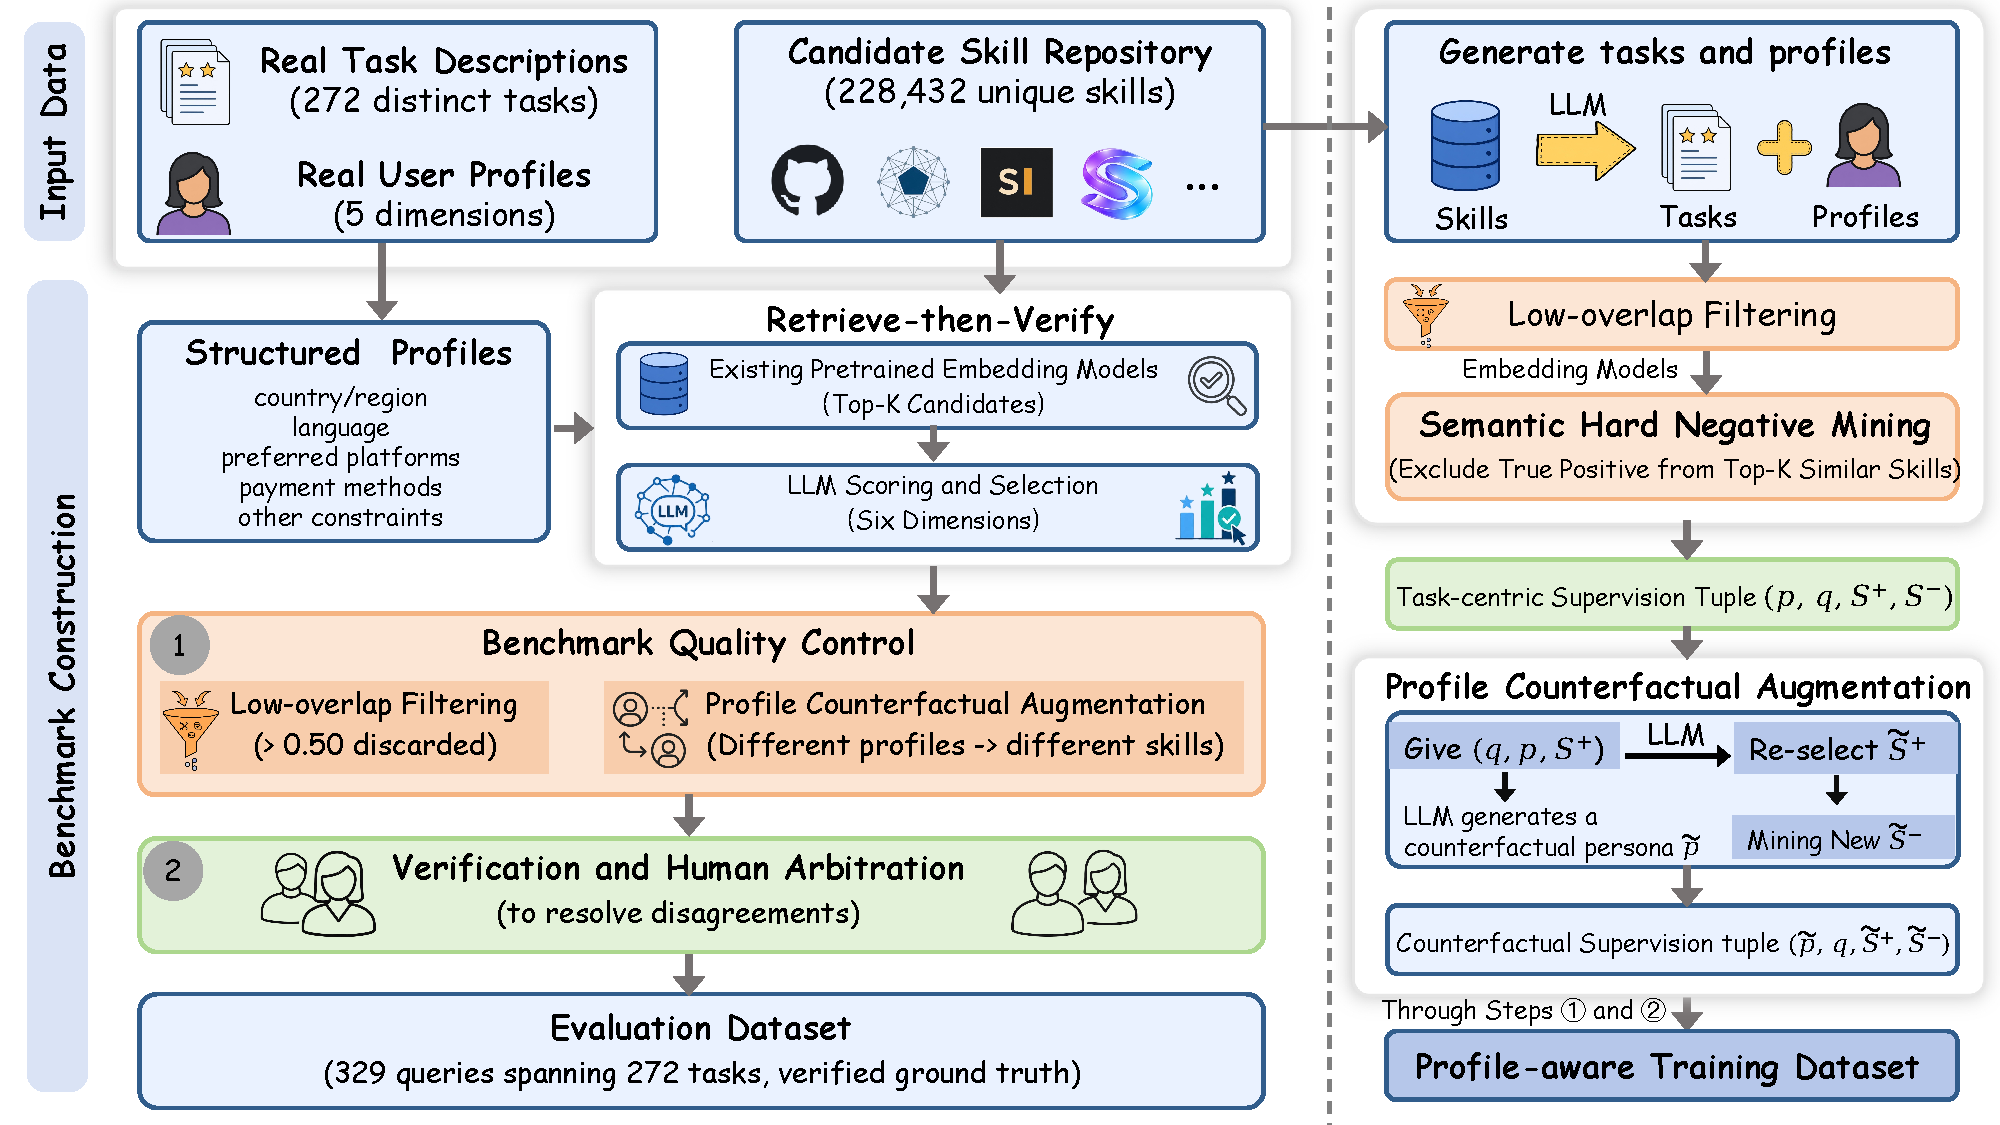
\includegraphics[width=0.8\textwidth]{Figures/fig3.pdf}
    \caption{Overview of the dataset construction pipeline. }
    \label{fig:benchmark}
\end{figure*}
% To bridge this gap, we introduce \textbf{SkillFeed-Bench}, a benchmark specifically designed to evaluate user-profile-based skill recommendations. The benchmark is
% constructed over a repository of 228{,}432 community-contributed skills and comprises 329 evaluation queries spanning 272 distinct tasks, each annotated with a ground-truth
% skill selected from the pool. Each query includes a task description and a structured user profile specifying country, language, domain, and other contextual constraints. This design enables systematic assessment of whether a retrieval model can identify skills that satisfy both the task requirements and the user-specific context.
This section formalizes \textit{personalized skill routing}, a setting in which the correct skill is determined jointly by the task and the user profile rather than by task semantics alone. 
Under a fixed task, changing user profile constraints may change the annotated reference skill, which makes conventional task-only evaluation insufficient. 
Therefore, we instantiate this setting with SkillFeed-Bench, a benchmark built over 228,432 community-sourced skills and 329 evaluation queries spanning ten domains, each paired with a structured user profile and an annotated reference skill.

%\liu{This paragraph seems to emphasize the benchmark a bit too much}

%\liu{This section first formalizes \textit{persona-conditioned skill routing}, a setting in which the correct skill is determined jointly by the task and the user profile rather than by task semantics alone. Under a fixed task, changing persona constraints may change the ground-truth skill, which makes conventional task-only evaluation insufficient. We therefore instantiate this setting with SkillFeed-Bench, a benchmark built over 228,432 community-sourced skills and 329 evaluation queries spanning ten domains, each paired with a structured persona profile and an annotated ground-truth skill.}

% Building on this formulation, we introduce SkillFeed-Bench, a benchmark specifically designed to evaluate -aware skill recommendation. SkillFeed-Bench is constructed from a repository of 228,432 community-sourced skills and comprises 329 evaluation queries spanning ten domains, ranging from development and research to lifestyle. Each query is annotated with a ground-truth skill selected from the skill repository. Every query consists of a task description paired with a structured user profile that specifies country, language, domain, and other contextual constraints.

\subsection{Personalized Skill Routing Formulation}

% We formulate \textit{Personalized Skill Routing} as the task of retrieving the most suitable skill conditioned on both the user task and the user persona.

% Let $q$ denote a user query, consisting of a task title, a natural-language description, and the desired execution objective. Let $p$ denote the user persona, represented as a structured collection of contextual attributes:

% \begin{equation}
% p=(c,l,\pi,e,\delta,\ldots),
% \end{equation}

% where $c$ denotes the user's country or region, $l$ the preferred language, $\pi$ the preferred platform or technology ecosystem, $e$ the user's expertise or professional background, and $\delta$ other task-relevant constraints (e.g., regulatory requirements, budget limitations, or domain-specific preferences). This representation is extensible and can naturally incorporate additional persona attributes.

% Let $\mathcal{S}=\{S_1,S_2,\ldots,S_N\}$ denote a repository of candidate skills. Each skill is a reusable procedural module for LLM agents that encapsulates a complete workflow for solving a class of tasks. It defines not only a sequence of execution steps, but also tool usage strategies, a\%licability conditions, and execution constraints.

% Given a query $q$, a persona $p$, and the candidate repository $\mathcal{S}$, the objective is to retrieve the most suitable skill

% \begin{equation}
% S^*=\arg\max_{S_i\in\mathcal{S}}f(q,p,S_i).
% \end{equation}

% % where $f(\cdot)$ measures the suitability of a candidate skill with respect to both the task requirements and the user's persona.

% % Unlike conventional skill routing, which assumes a universal ma\%ing from task to skill,

% % \begin{equation}
% % T \rightarrow S,
% % \end{equation}

% % personalized skill recommendation explicitly models

% % \begin{equation}
% % (T,p)\rightarrow S,
% % \end{equation}

% % allowing identical tasks to be ma\%ed to different skills under different user personas.
% %  近似独立 约等于 不考虑技能组合层面的协同或冲突效应。
% 
% \begin{equation}
% \Pr\!\left[S^*_{q,p} \subseteq \text{top-}K \mid q,p\right]
% \approx
% \prod_{s \in S^*_{q,p}}
% \Pr\!\left[s \in \text{top-}K \mid q,p\right]
% \quad 
% \end{equation}


% \begin{equation}
% \mathcal{R}_K(q,p) = \text{TopK}_{s \in \mathcal{S}} f(q,p,s)
% \end{equation}


% \begin{equation}
% \mathbb{I}\left[S^*_{q,p} \subseteq \mathcal{R}_K(q,p)\right]
% \end{equation}

Let $q$ denote a natural-language task query, $p$ a structured user profile, and $\mathcal{S}=\{S_1,\ldots,S_N\}$ a repository of candidate skills. The profile contains only task-relevant contextual attributes, such as country or region, language, platform access, payment method, expertise, and other constraints. Each candidate skill $S_i=(n_i,d_i,b_i)$ comprises a name $n_i$, a concise description $d_i$, and a procedural body $b_i$ that specifies its workflow and applicability conditions.

Personalized skill routing selects the candidate that best satisfies the task and profile jointly:
\begin{equation}
S_{q,p}^{*}
=
\arg\max_{S_i\in\mathcal{S}}
f(q,p,S_i),
\label{eq:personalized_skill_routing}
\end{equation}
where $f(q,p,S_i)$ measures the compatibility of $S_i$ with both $q$ and $p$. This differs from task-only routing: a skill can be semantically relevant to $q$ yet unsuitable because it conflicts with the profile's constraints.

For scalable retrieval, the system ranks all candidates by this score and returns the top-$K$ set:
\begin{equation}
\mathcal{R}_K(q,p)
=
\operatorname{TopK}_{S_i\in\mathcal{S}}
f(q,p,S_i),
\label{eq:personalized_topk_routing}
\end{equation}
where $\mathcal{R}_K(q,p)$ is the ordered set of the $K$ highest-ranked skills for $(q,p)$. Because each evaluation instance has one annotated reference skill, candidate recall succeeds when $S^*_{q,p}\in\mathcal{R}_K(q,p)$.


\iffalse
\textit{Personalized skill routing} is formulated as a user profile-conditioned
retrieval problem over a repository of candidate skills. Given a user query
$q$, a user profile $p$, and a skill repository
$\mathcal{S}$, the objective is to identify the skill
that best satisfies both the task requirements specified by $q$ and the user profile $p$. Formally,
the optimal skill is defined as
\begin{equation}
S_{q,p}^{*}
=
\arg\max_{S_i\in\mathcal{S}}
f(q,p,S_i),
\label{eq:personalized_skill_routing}
\end{equation}
where $f(q,p,S_i)$ is a user profile-conditioned scoring function that measures
the compatibility of candidate skill $S_i$ with the task $q$ and the user profile $p$.

The user query $q$ describes the task to be performed and consists of a task title and a description in natural-language.
The user profile $p$  is represented as a structured collection of contextual attributes, such as language preference, and professional background, among others.
% The user profile $p$ is represented as a structured collection of contextual attributes:
% \begin{equation}
% p=(c,l,\pi,e,\delta,\ldots),
% \label{eq:persona_representation}
% \end{equation}
% where $c$ is the user's country or region, 
% $l$ is the preferred language, 
% $\pi$ is the preferred platform or technology ecosystem, 
% $e$ is the user's expertise or professional background, 
% and $\delta$ is other task-relevant constraints (e.g., regulatory requirements, budget limitations, or domain-specific preferences). 
% This representation is extensible and can incorporate additional user profile attributes when required.

The repository $\mathcal{S}$ contains $N$ candidate skills. Each skill is
represented as a triplet $S_i=(n_i,d_i,b_i),$ where $n_i$ is the skill name, $d_i$ is a concise description of its
functionality, and $b_i$ is its complete procedural body. 

% In contrast to conventional task-level skill retrieval, which ranks candidate skills
% solely according to their relevance to the query $q$, personalized skill
% routing additionally considers their compatibility with the user profile $p$.
% Consequently, a skill that is semantically relevant to a task may not be the most suitable choice when it conflicts with the user's platform, language,
% expertise, or other contextual constraints.
Personalized skill routing adds user-profile $p$ compatibility to task $q$ relevance, so a semantically relevant skill may still be unsuitable if it conflicts with the user's constraints.

In practice, the routing formulation ranks all candidate skills according to their
user profile-conditioned compatibility scores and returns the top-$K$ candidates:
\begin{equation}
\mathcal{R}_K(q,p)
=
\operatorname{TopK}_{S_i\in\mathcal{S}}
f(q,p,S_i),
\label{eq:personalized_topk_routing}
\end{equation}
where $\mathcal{R}_K(q,p)$ is the ordered set of the $K$ highest-ranked
skills for the query--profile pair $(q,p)$.


%\textit{Personalized skill routing} is proposed as a new retrieval paradigm, where the objective is to select the most suitable skill conditioned on both the user query and the user persona.

%Let $q$ denotes a user query, consisting of a task title, a natural-language description, and the desired execution objective. Let $p$ denotes the user persona, represented as a structured collection of contextual attributes:
%\begin{equation}
%p=(c,l,\pi,e,\delta,\ldots),
%\end{equation}
%where $c$ is the user's country or region, $l$ is the preferred language, $\pi$ is the preferred platform or technology ecosystem, $e$ is the user's expertise or professional background, and $\delta$ is other task-relevant constraints (e.g., regulatory requirements, budget limitations, or domain-specific preferences). This formulation is extensible and readily accommodates additional persona attributes.
% What does a skill look like? A typical skill contains:  • name: a short identifier, e.g. SendGrid Email Send; • description: a one-line purpose, e.g. “Send transactional emails through SendGrid”;  • body: detailed call instructions (API shape, parameter constraints, platform dependencies, best practices, canonical code), typically tens to hundreds of lines.

% Let $\mathcal{S}=\{S_1,S_2,\ldots,S_N\}$ denote a repository of candidate skills. 
% Each skill is a reusable triplet $S_i = (n_i, d_i, b_i)$ for LLM agents that encapsulates a complete workflow for solving a class of tasks, where $n_i$ and $d_i$ are a short name and a one-line purpose, while $b_i$ is an extensive procedural body---spanning hundreds of lines with API specifications, dependencies, and code examples---that encapsulates the complete execution workflow and applicability constraints for LLM agents.

%Let $\mathcal{S} = \{S_1, S_2, \ldots, S_N\}$ denote a repository of candidate skills. Each skill is a triplet $S_i = (n_i, d_i, b_i)$, where $n_i$ and $d_i$ are a short name and a one-line description, and $b_i$ is an extensive procedural body with API specifications, dependencies, and code examples that encapsulates the complete execution workflow and applicability constraints for LLM agents.

% Given a query $q$, a persona $p$, and the candidate repository $\mathcal{S}$, the objective is to retrieve the most suitable skill

%In contrast to conventional task-level skill retrieval that relies solely on the query $q$, personalized skill routing fundamentally conditions on the user persona $p$: given a query $q$, a persona profile $p$, and the candidate repository $\mathcal{S}$, the objective is to retrieve the skill $S_i \in \mathcal{S}$ that best satisfies both the task requirement and the persona-induced constraints.

%\begin{equation}
%S^*_{q,p}=\arg\max_{S_i\in\mathcal{S}}f(q,p,S_i),
%\end{equation}
%where $f(\cdot)$ denotes a scoring function measuring the compatibility between the task, the user persona, and the candidate skill.
% \liu{"where" should not start a new paragraph}
% \wang{fixed}

%In practice, retrieval is performed by ranking all candidate skills and selecting the top-$K$ candidates:

%\begin{equation}
%\mathcal{R}_K(q,p)
%=
%\operatorname{TopK}_{s\in\mathcal{S}}
%f(q,p,s).
%\end{equation}
% 与\cite{wang2026r3skill}不同 在本工作中，我们主要聚焦于如何引入 Persona ($p$) 来提升 Routing 的个性化和精准度。为了简化检索模型的训练目标，我们假设在给定 $(q, p)$ 的强上下文中，各个技能的召回概率是条件独立的。我们暂不引入技能间的联合概率或排斥校验（即忽略兼容性修正项）


% \liu{why we need the following paragraph?}
% \wang{Since I used their formula, but we didn't take certain factors into account, I need to provide an explanation. maybe we should delete this formula }
% Furthermore, unlike \cite{wang2026r3skill}, which explicitly models inter-skill compatibility and joint retrieval probabilities, this work concentrates on user profile conditioned routing. To keep the training objective tractable, we assume conditional independence among individual skill retrieval events given the strong context $(q, p)$, deliberately omitting compatibility correction terms and inter-skill joint probabilities. Under this simplification, the retrieval objective can be approximated as:

% \begin{equation}
% \Pr\!\left[
% S^*_{q,p}\subseteq\mathrm{top}\text{-}K
% \mid q,p
% \right]
% \approx
% \prod_{s\in S^*_{q,p}}
% \Pr\!\left[
% s\in\mathrm{top}\text{-}K
% \mid q,p
% \right].
% \end{equation}

Finally, retrieval succeeds if every annotated skill is contained in the retrieved candidate set, which is represented by the indicator function

\begin{equation}
\mathbb{I}\!\left[
S^*_{q,p}\subseteq
\mathcal{R}_K(q,p)
\right].
\end{equation}
\fi

% \paragraph{Key Challenge.}

% The central challenge is that the optimal skill is not uniquely determined by task semantics. While conventional retrieval methods estimate relevance solely based on task--skill semantic matching,

% \begin{equation}
% f(T,p,S)\neq g(\mathrm{sim}(T,S)),
% \end{equation}

% where $g(\cdot)$ denotes a persona-agnostic relevance function. In personalized skill recommendation, the suitability of a skill additionally depends on its compatibility with the user's contextual constraints. Consequently, effective recommendation requires jointly modeling task semantics and persona-specific preferences, rather than relying solely on semantic similarity.

\subsection{SkillFeed-Benchmark Construction}

\paragraph{Data Sources.}
% The candidate skill repository is constructed by aggregating skills from many different sources such as github, SkillNet~\cite{liang2026skillnetcreateevaluateconnect}, and SkillSMP~\cite{skillsmp2026}. Following deduplication and format normalization, a pool of 228,432 skills is obtained, each containing a name, description, and body content.
We aggregate skills from public sources, including GitHub, SkillNet~\cite{liang2026skillnetcreateevaluateconnect}, and SkillSMP~\cite{skillsmp2026}. After deduplication and format normalization, the repository contains 228,432 skills, each with a name, description, and procedural body.

\paragraph{Task and Profile Collection.}
We collect task descriptions from real LLM-agent interactions in which users sought help with specific goals. After manual screening for self-containedness, sufficient detail, and practical relevance, we retain 272 unique tasks. Each task is paired with a structured user profile covering country or region, language, preferred platforms, payment methods, and additional constraints such as regulatory requirements, budget limits, or domain-specific workflows. The profiles are designed to be concise while retaining attributes that can affect skill suitability.

% The collection of task descriptions is originated from real LLM agent interactions, where users sought assistance for specific goals. Each description is manually verified for self‑containedness, sufficient detail, and representativeness of practical usage scenarios, yielding 272 unique tasks. Subsequently, each task is annotated with a structured user profile covering five dimensions: country/region, language, preferred platforms, payment methods, and additional constraints (e.g., regulatory requirements, budget limits, domain‑specific workflows). The profiles are deliberately kept minimal yet decision‑relevant, ensuring that any single constraint can affect the optimal skill recommendation for that task.

\paragraph{Reference Target Annotation.}
\label{para:gt annotation}
Exhaustive annotation over 228,432 skills is impractical. We therefore use a two-stage annotation procedure. First, pretrained embedding models retrieve a top-$K$ set of semantically relevant candidates for each task--profile pair. Second, an LLM assesses these candidates using task relevance, profile compatibility, capability match, constraint satisfaction, specificity, and overfit risk, and then performs pairwise comparisons to select the reference skill. Each annotated instance is a triplet $(p,q,S)$ consisting of a profile, task query, and selected skill.

% Given the large candidate pool of 228,432 skills, exhaustive human annotation is impractical. A two‑step procedure is therefore adopted: for each task under a given user profile, existing pretrained embedding models first retrieved the top‑$K$ semantically similar candidates, reducing the annotation space to a manageable number; then an LLM scores those candidates along six dimensions, including task relevance, user profile compatibility, capability match, constraint satisfaction, specificity, and overfit risk, and performed pairwise comparison to select the  the annotated reference target.The resulting output for each task under a given profile is a triplet $(p, q, S)$ comprising the profile, the task query, and the selected skill.

\paragraph{User Profile Counterfactual Augmentation.}
% \liu{"Persona Counterfactual Augmentation" is too long; you can write a simplified version here and put the specific details in the appendix}
% 经过标注的triplet $(p, q, S)$ 中task和persona对skill选择的影响相互耦合，无法区分各自的贡献。为在数据层面解耦persona的独立效应，我们采用Persona Counterfactual Augmentation的策略，通过构造反事实样本，固定task、改变persona，从而单独考察persona对skill选择的影响。
% 具体而言，给定一个原始标注triplet $(p, q, s^{+})$（其中 $p$ 表示原始用户画像），我们利用大型语言模型生成一个合理的反事实用户画像 $\tilde{p}$，该画像虽与原始画像不同，但仍符合现实中的用户特征。在 $(\tilde{p}, q)$ 的条件下，重复Ground Truth Annotation 的操作,我们技能库中重新选择最合适的技能 $\tilde{s}^{+}$. 为了确保反事实样本的有效性，我们严格过滤掉 $\tilde{s}^{+} = s^{+}$ 的情况，仅保留因画像改变而导致最优技能发生实质性改变的样本。
% 由此我们可以得到新的从而得到一个新的triplet $(\tilde{p}, q, \tilde{s}^{+})$ 这一过程有效丰富了 benchmark 在多样化画像下的评估难度。

For an ordinary triplet $(p,q,S)$, the effects of the task and profile are coupled. We therefore construct counterfactual instances that hold $q$ fixed while varying $p$. Given an original instance, we prompt an LLM to generate a plausible alternative profile $\tilde{p}$ that deviates from the original $p$ and reapply the reference-target annotation procedure to $(\tilde{p},q)$. We retain the resulting triplet $(\tilde{p},q,\tilde{S})$ only when $\tilde{S}\neq S$. These retained pairs directly test whether a routing method changes its prediction when a profile change alters the suitable skill.

% In the annotated triplets $(p, q, S)$, the effects of the task and the user profile on skill selection are coupled, making it difficult to disentangle their respective contributions. To decouple the independent effect of the user profile from that of the task at the data level, we adopt a User Profile Counterfactual Augmentation strategy. This approach constructs counterfactual examples by fixing the task while varying the profile, thereby enabling isolated examination of the profile's influence on skill selection. Specifically, given an original annotated triplet $(p, q, S)$, where $p$ denotes the original profile, we prompt an LLM to generate a plausible counterfactual profile $\tilde{p}$ that deviates from the original while preserving realistic user characteristics. Conditioned on $(\tilde{p}, q)$, we re-select the most appropriate skill $\tilde{S}$ from the skill repository, following the same annotation procedure described in Section \ref{para:gt annotation}. To ensure the validity of the counterfactual samples, we filter out instances where $\tilde{S} = S$, retaining only those where the user profile variation induces a substantive shift in the optimal skill. This yields a new triplet $(\tilde{p}, q, \tilde{S})$ for each retained instance, effectively enriching the benchmark with evaluation scenarios that span diverse user profiles.

% Although the above supervision captures semantic relevance, it does not model the effect of user personas on skill selection. In practice, users with different backgrounds or preferences may choose different skills even for the same task. To introduce persona-sensitive supervision, we generate counterfactual training examples by modifying the user persona while keeping the task unchanged.

% Specifically, given an original training instance $(p, q, s^{+})$, where $p$ denotes the original persona, we employ a large language model to generate a plausible counterfactual persona $\tilde{p}$ that differs from the original one while remaining consistent with realistic user profiles. Conditioned on $(\tilde{p}, q)$, the language model then re-selects the most a\%ropriate skill $\tilde{s}^{+}$ from the skill repository. Hard negative skills are subsequently mined following the same strategy described above, resulting in a new supervision tuple

% \[
% (\tilde{p}, q, \tilde{s}^{+}, \tilde{\mathcal{S}}^{-}).
% \]

% The counterfactual augmentation enables the retriever to observe how variations in user personas lead to different skill selections under an identical task, thereby encouraging persona-aware retrieval behaviors.

% Finally, the original task-centric supervision and the generated counterfactual supervision are combined to form the final persona-aware training dataset,

% \[
% \mathcal{D}
% =
% \mathcal{D}_{\mathrm{orig}}
% \cup
% \mathcal{D}_{\mathrm{cf}},
% \]

% which provides diverse supervision over both semantic relevance and persona-specific preferences. This enriched training data serves as the foundation for learning a retriever that jointly models task semantics and personalized user characteristics.


% \paragraph{Low-overlap Filtering.}
% \liu{this part is not very clear and too long}

% The original Task--Skill pairs collected from real-world interactions inevitably contain many trivial samples where the task description explicitly reveals the target skill (e.g., ``translate text'' paired with ``Translator''). Such lexical shortcuts encourage the retriever to rely on surface-level word matching instead of semantic understanding. Therefore, we first compute lexical overlap between each task and its corresponding skill description using token-level similarity metrics and remove pairs whose overlap exceeds a predefined threshold. The remaining samples require semantic reasoning for correct retrieval and serve as high-quality positive instances.

% To further ensure annotation quality, we apply the same low-overlap filtering and counterfactual augmentation strategies described in
% Section~\ref{subsection:Persona-aware Supervision Construction}: we discard task--skill pairs with lexical overlap exceeding 0.50 to eliminate trivial shortcuts, and augment the benchmark
% with persona counterfactual examples where the same task paired with different personas yields different ground-truth skills. All LLM-generated labels and counterfactual
% variants are independently verified by at least two human annotators; disagreements are resolved through expert arbitration, and ambiguous cases are discarded. 
% % This process yields 329 evaluation queries spanning 272 distinct tasks, each annotated with a verified ground-truth skill from the 228K pool.


\paragraph{Quality Control.}
% 我们保证llm生成的反事实用户画像 和筛选出来的ground truth都经过人工审核
% \liu{
% To ensure that SkillFeed-Bench evaluates persona-conditioned routing rather than superficial matching, we apply two quality-control steps. First, we reduce lexical shortcuts by computing overlap between each task and its corresponding skill description and discarding pairs whose overlap exceeds 0.50; the remaining samples require stronger semantic reasoning and better reflect the intended routing setting. Second, all LLM-assisted labels and counterfactual variants are independently verified by at least two human annotators, with disagreements resolved through expert arbitration and ambiguous cases discarded. Together, these steps improve the reliability of both standard and persona-sensitive routing instances.}
% To ensure that SkillFeed-Bench evaluates persona-conditioned routing rather than merely task-level semantic matching, we integrate quality controls throughout the construction pipeline. Concretely, we apply automated screening to all LLM-generated candidates: samples with confidence scores below 0.80 are discarded, and task--skill pairs whose token-level overlap exceeds 0.50 are eliminated, as such pairs admit trivial keyword-based solutions and thus allow correct retrieval without genuine persona-aware reasoning. For counterfactual variants, we additionally enforce logical consistency by verifying that the generated persona attributes do not contradict the content or category of the newly assigned ground-truth skill. Furthermore, to prevent data leakage, we perform dataset partitioning based on the hash of the original task content rather than the sample identifier, ensuring that all derivations of the same source task are confined to a single split. Finally, all retained original and counterfactual samples are independently evaluated by at least two human annotators. Any annotation discrepancies are resolved via expert arbitration, and persistently ambiguous cases are excluded. Collectively, these measures guarantee that each evaluation instance constitutes a genuine, persona-aware routing challenge rather than a reflection of spurious correlations or annotation artifacts.

We apply quality controls to ensure that SkillFeed-Bench tests profile-conditioned routing rather than superficial task level semantic matching. We discard samples with confidence scores below 0.80 and task--skill pairs with lexical overlap above 0.50, reducing trivial keyword matches and evident annotation errors. We then apply consistency checks and manually review retained instances. At least two professional human annotators with prior experience in evaluating AI agents, software tools, or programming-related tasks independently evaluate every retained original and counterfactual instance; expert arbitration resolves disagreements, and persistently ambiguous cases are excluded. These procedures reduce the risk that benchmark performance reflects spurious lexical cues or annotation artifacts.
% 参考skillnet的方法 我们对生成的数据进行了统计分析 Category如图所示

% \liu{we can put this statistical analysis into appendix}
% As a result, we construct SkillFeed, a counterfactual benchmark consisting of a 228K skill pool and 329 evaluation queries spanning diverse task domains. 
The resulting benchmark contains 329 evaluation queries over 228K candidate skills, including 162 profile-sensitive queries (77 profile-counterfactual augmentation) and 167 profile-insensitive queries. Sensitive and Insensitive subsets are defined by
presence of user context constraints.
% The resulting benchmark contains 329 evaluation queries over 228K candidate skills, including 77 profile-sensitive queries produced by profile-counterfactual augmentation and 252 profile-insensitive queries. 
Its controlled profile shifts expose a routing problem that task-only methods cannot resolve: a system must revise its selected skill when the user profile changes the suitable execution path, while still retrieving efficiently. 
SkillFeed-Bench is therefore architecture-agnostic, but it demands balancing  broad recall for its vast pool with fine-grained discrimination for user profile shifts. We next present SkillFeed, a two-stage retrieval-and-reranking approach designed to meet these requirements and evaluated on this benchmark.
%  but it requires routing methods to jointly model task relevance and profile compatibility rather than task semantics alone.
 % 因此，SkillFeed-Bench 是一种与架构无关的方案，但它需要路由方法同时建模任务相关性和个人资料兼容性，而不仅仅是任务语义。接下来，我们将介绍 SkillFeed——一种旨在满足这些要求并在该基准测试上经过评估的两阶段方法。


% SkillFeed-Bench 实现了基于用户画像的技能路由机制。其庞大的候选技能库需要高效的检索能力，而受控的用户画像变化场景则要求对那些与任务相关性相似、但在满足用户约束条件方面存在差异的技能进行精细区分。这些互补的需求促使我们采用两阶段设计，将广泛的候选技能检索与基于用户画像的重新排序分离。基于这一基准测试框架，下一节将介绍 SkillFeed 及其基于用户画像的训练策略。
% The resulting benchmark contains 329 evaluation queries over 228K candidate skills, including 77 profile-sensitive queries produced by profile-counterfactual augmentation and 252 profile-insensitive queries. 
% Its controlled profile shifts expose a routing challenge that task-only methods cannot resolve: a system must dynamically revise its skill selection when the user profile alters the viable execution path, while maintaining retrieval efficiency. 
% Consequently, while SkillFeed-Bench remains architecture-agnostic, it necessitates routing methods that jointly model task relevance and profile compatibility rather than task semantics alone. We next present SkillFeed, a two-stage approach designed to meet these exact requirements.

% While architecture-agnostic, the benchmark inherently demands balancing efficient broad recall for its vast pool with fine-grained discrimination for profile shifts. To jointly model task relevance and profile compatibility under this tension, we next present SkillFeed, a two-stage retrieval-and-reranking approach.
% \iffalse
% To ensure that SkillFeed-Bench evaluates user profile-conditioned routing rather than merely task-level semantic matching, we integrate rigorous quality controls throughout the construction pipeline. Initially, we apply confidence and lexical-overlap filters, followed by consistency checks and manual review of retained cases. Samples with confidence scores below 0.80 are discarded, and pairs of tasks and skills exhibiting a lexical overlap above 0.50 are eliminated. These steps reduce trivial lexical matches and obvious annotation errors. Finally, all retained original and counterfactual samples are independently evaluated by at least two human annotators. Expert arbitration resolves any discrepancies, while persistently ambiguous cases are excluded. Collectively, these protocols help reduce the risk of spurious correlations and annotation artifacts, supporting each instance as a reasonable test of routing capability.
% % 参考skillnet的方法 我们对生成的数据进行了统计分析 Category如图所示

% % \liu{we can put this statistical analysis into appendix}
% % As a result, we construct SkillFeed, a counterfactual benchmark consisting of a 228K skill pool and 329 evaluation queries spanning diverse task domains. 
% As a result, we construct SkillFeed-Bench over a pool of 228K candidate skills, with 329 evaluation queries spanning diverse task domains. The benchmark contains 77 profile-sensitive queries generated through profile-counterfactual augmentation and 252 standard queries treated as profile insensitive queries.
% % Appendix Figure~\ref{fig:category_distribution} presents the distribution of skill categories, demonstrating the broad coverage of the benchmark across different application domains.



% % \section{Method: SkillFeed}
% % \begin{figure*}[htbp]
% %     \centering
% %     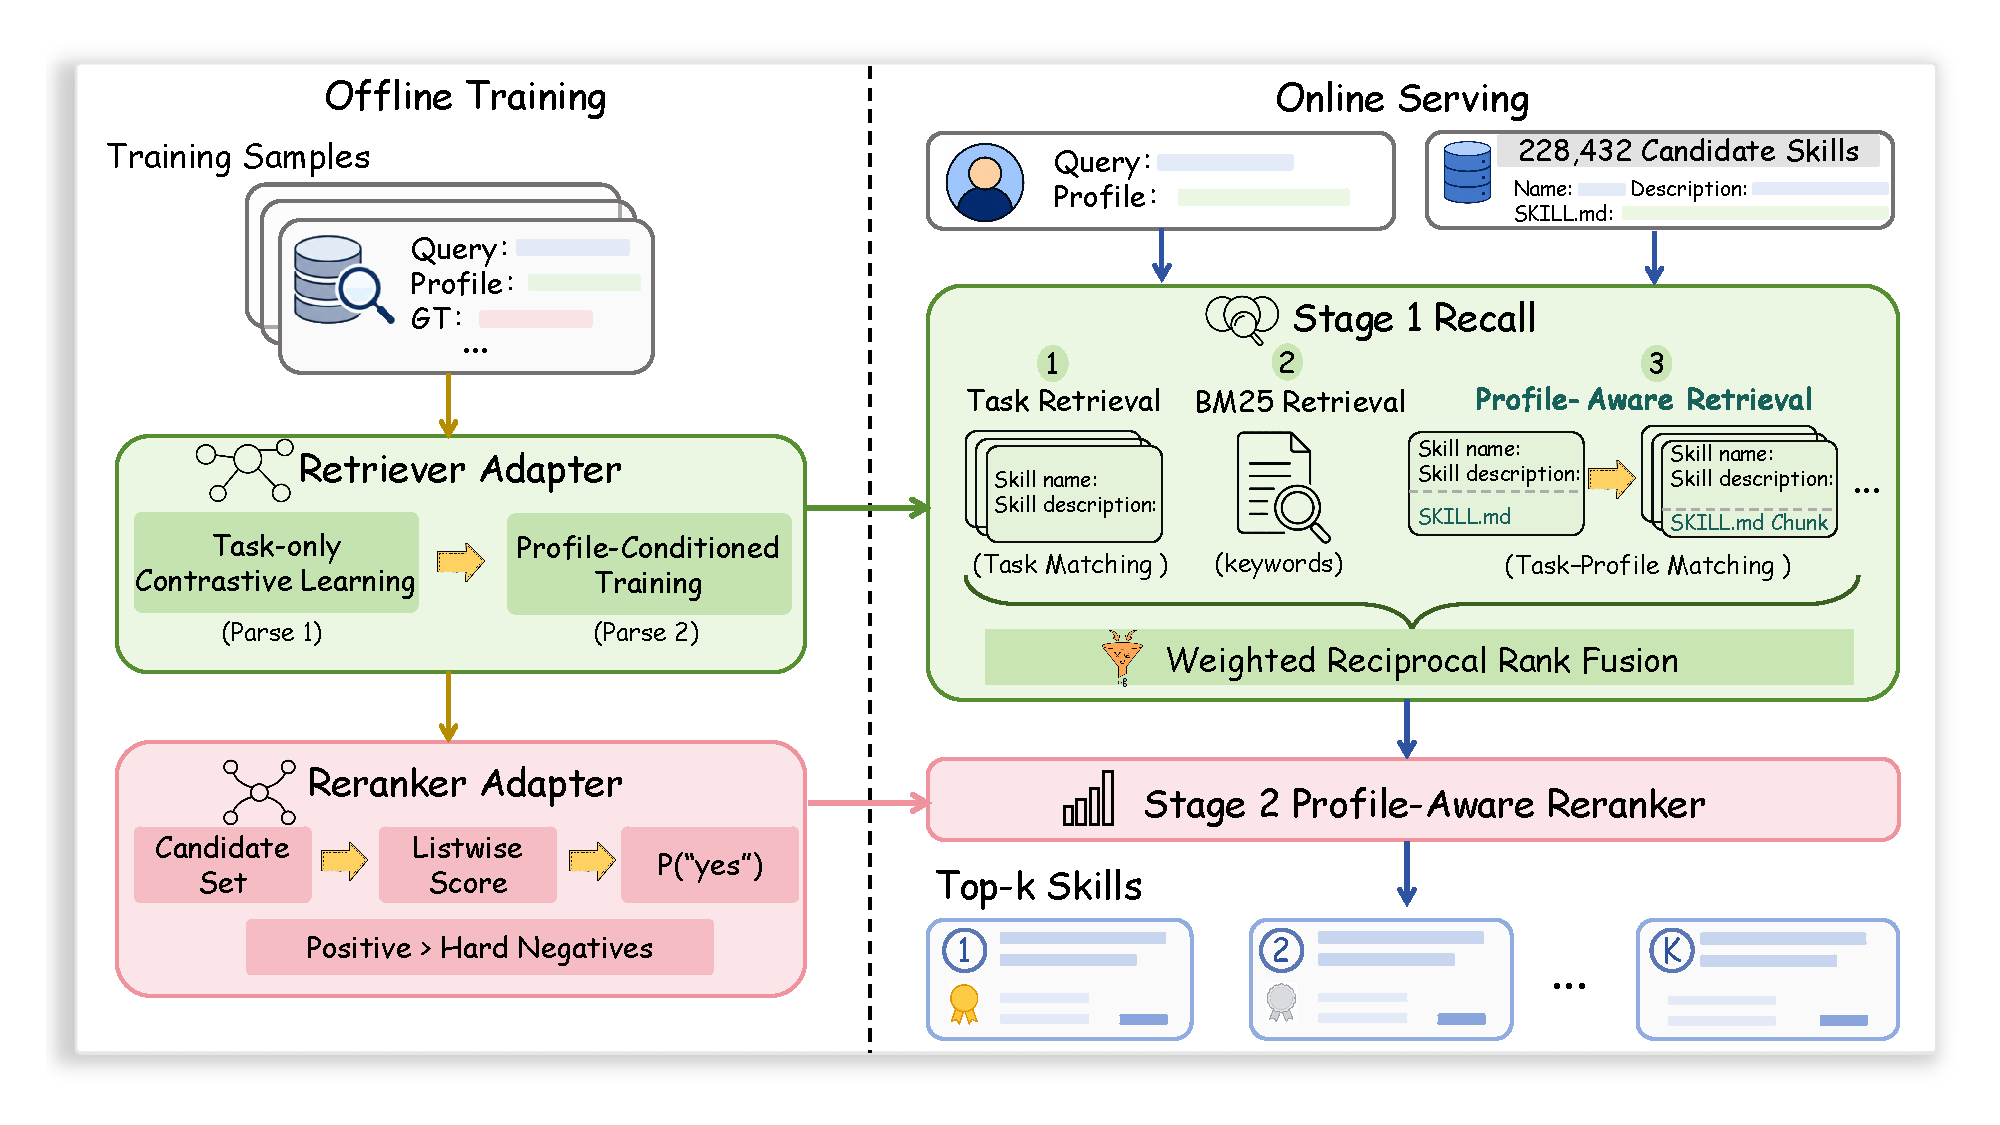
\includegraphics[width=0.95\textwidth]{Figures/fig2.pdf}
% %     \caption{Method of personalized skill recommendation.}
% %     \label{fig:method}
% % \end{figure*}

% % \liu{Based on this benchmark, a description needs to be written that traditional methods clearly fail in dealing with this type of problem}
% % 我们在SkillFeed-Bench上的实验结果表明，虽然传统检索方法在任务级语义匹配方面表现有效，但在个性化技能路由场景中，其性能会显著下降。具体而言，这些方法仅基于任务-技能对进行训练，相似度计算的重点在于任务描述和技能元数据，忽略了用户属性信息。导致构建的语义匹配空间中存在bias。这一缺陷要求必须基于用户画像感知数据对检索模型进行微调，以编码联合的（任务、用户画像）语义空间，这自然催生了一种两阶段架构：首先使用密集检索器进行粗略过滤，随后使用重新排序器进行精细区分。SkillFeed-Bench由此为评估此类角色感知技能路由系统提供了一个严格的测试平台。
% % Experiments on SkillFeed-Bench demonstrate that while conventional retrieval methods exhibit high efficacy in task-level matching, they struggle with personalized skill routing. Trained exclusively on task-centric data and remaining agnostic to user profiles, these methods inevitably introduce biases into the semantic space during personalized skill matching. Addressing this requires fine-tuning on user profile-aware data to encode the joint (task, profile) space, which naturally motivates a two-stage retrieve and rerank architecture. SkillFeed-Bench serves as a rigorous testbed for evaluating such profile-aware routing systems.
% SkillFeed-Bench operationalizes profile-conditioned skill routing at repository scale. Its large candidate pool requires efficient recall, whereas its controlled profile-shift cases require fine-grained discrimination among skills that are similarly relevant to the task but differ in their compatibility with user constraints. These complementary requirements motivate a two-stage design that separates broad candidate retrieval from profile-conditioned reranking. Building on this benchmark formulation, the next section introduces SkillFeed and its profile-aware training strategy.
% \fi

% 有位置再加
% \paragraph{Standard Ranking Metrics.}
% Given a query $q$ and a ranked list of retrieved skills $\mathcal{R}_K(q)$, Hit@K is defined as:
% \begin{equation}
% \text{Hit@K} = \mathbb{1}[s^{*} \in \mathcal{R}_K(q)],
% \end{equation}
% where $s^{*}$ denotes the ground-truth skill. Mean Reciprocal Rank is defined as:
% \begin{equation}
% \text{MRR} = \frac{1}{N} \sum_{i=1}^{N} \frac{1}{\text{rank}_i(s^{*})}.
% \end{equation}


% \paragraph{Coverage@K.}
% Given the large candidate space of 228K skills, we additionally report Coverage@K, defined as:
% \begin{equation}
% \text{Coverage@K} = \frac{1}{N} \sum_{i=1}^{N} \mathbb{1}[s^{*}_i \in \mathcal{R}_K(q_i)],
% \end{equation}
% which measures whether the retriever successfully surfaces the ground-truth skill from the full repository.

% \paragraph{Counterfactual Consistency.}
% To evaluate sensitivity to persona variations, we define Counterfactual Consistency over persona groups. Let $\mathcal{G}$ denote a group of instances sharing the same task but with different persona settings. The model is consistent if it retrieves the correct top-1 skill for all persona variants:
% \begin{equation}
% \text{CC} = \frac{1}{|\mathcal{G}|} \sum_{g \in \mathcal{G}} \prod_{(q,p) \in g} \mathbb{1}[\text{rank}_1(s^{*}_{q,p}) = 1].
% \end{equation}

% This metric measures whether the model adaptively adjusts its predictions under persona changes, rather than relying solely on task semantics.


\section{Method: SkillFeed}




% 在本节中，我们提出了一种用于个性化技能推荐的框架。首先，我们定义了该任务，并分析了使其有别于传统技能检索的基本挑战。由于最优技能既取决于任务语义，又取决于用户特有的上下文约束，因此仅基于语义相关性进行训练的现有检索模型无法捕捉受用户特征影响的技能偏好。
% 为应对这一挑战，我们提出了一个统一的训练与推理框架。首先，通过自动生成高质量的“task-persona-skill”训练实例，构建了专为基于用户画像的技能推荐量身定制的监督数据。基于生成的监督数据，我们同时优化了密集检索模型和重新排序模型，使其学习受用户画像影响的相关性，而非仅基于任务的语义相似性。最后，我们将训练好的模型集成到一个两阶段检索pipeline中，该pipeline能够高效地识别候选技能并执行精细的、基于用户画像的排序，从而实现针对大型技能库的可扩展个性化技能推荐。

% 基于SkillFeed-Bench，我们现提出一种Personalized Skill Routing 框架：SkillFeed。与依赖于忽视用户画像的任务中心检索方法不同，我们采用了一种两阶段的检索与重新排序架构， as illustrated in Figure~\ref{fig:method} 该架构明确建模了（任务、用户画像）的联合空间。为此，我们首先构建了高质量的训练样本，如图 \ref{fig:benchmark}右侧流程所示，将任务语义与特定用户画像的上下文约束相结合，从而自动生成用于用户画像感知技能推荐的监督数据。利用这些数据，我们对稠密检索器和跨编码器重新排序器进行了微调，使其学习受用户画像影响的相关性，而非仅基于任务的语义相似性。随后，这两个组件被整合到一个可扩展的处理流程中：检索器从大型库中高效检索候选技能，而重新排序器则执行精细的、基于用户画像的排序，以生成最终的个性化结果。该设计直接解决了传统方法中发现的偏差问题，并利用 SkillFeed-Bench 作为基于用户画像的路由系统的评估基准。

% This section presents SkillFeed, a framework for personalized skill routing. In contrast to task-centric retrieval methods, which rely exclusively on task-level semantic similarity and disregard user profiles, the proposed framework automatically constructs training instances by integrating task semantics with user-specific contextual constraints. These instances, generated independently from the benchmark, provide supervision signals for user profile-aware skill recommendation. Using these data, both a dense retriever and a cross-encoder reranker are fine-tuned to learn relevance measures conditioned on user profiles, rather than on task semantics alone. The two fine-tuned components are subsequently integrated into a scalable two-stage inference pipeline: the retriever efficiently recalls candidate skills from a large‑scale repository, and the reranker performs fine-grained user profile-based ranking to yield the final personalized recommendations. This design directly mitigates the biases inherent in conventional matching approaches, thus enabling effective user profile‑aware skill routing.

SkillFeed is designed around three requirements that distinguish profile-conditioned routing from conventional task-skill retrieval. First, a router must retain broad functional coverage over a large repository: profile information should refine task relevance rather than replace it. Second, the decisive profile constraint often separates skills that are already semantically similar, so the model needs supervision in which a fixed task maps to different skills under different profiles. Third, these constraints frequently occur in the procedural body of a skill rather than in its short description. As illustrated in Figure~\ref{fig:method}, SkillFeed addresses these requirements jointly: it constructs counterfactual profile supervision, learns task alignment before profile-sensitive discrimination, and retrieves body-level evidence before making a final profile-conditioned ranking. Thus, the components are not interchangeable retrieval add-ons; each resolves a distinct failure mode of task-only routing.

% SkillFeed constructs profile-aware supervision to adapt a dense retriever and a cross-encoder reranker for personalized skill routing. At inference time,
% three complementary recall channels---task-oriented dense retrieval, BM25, and profile-conditioned retrieval over \texttt{SKILL.md} chunks---produce a
% fused candidate set. The adapted reranker then models fine-grained compatibility among the task, user profile, and candidate skills to produce
% the final ranking.

\begin{figure}[t]
    \centering
    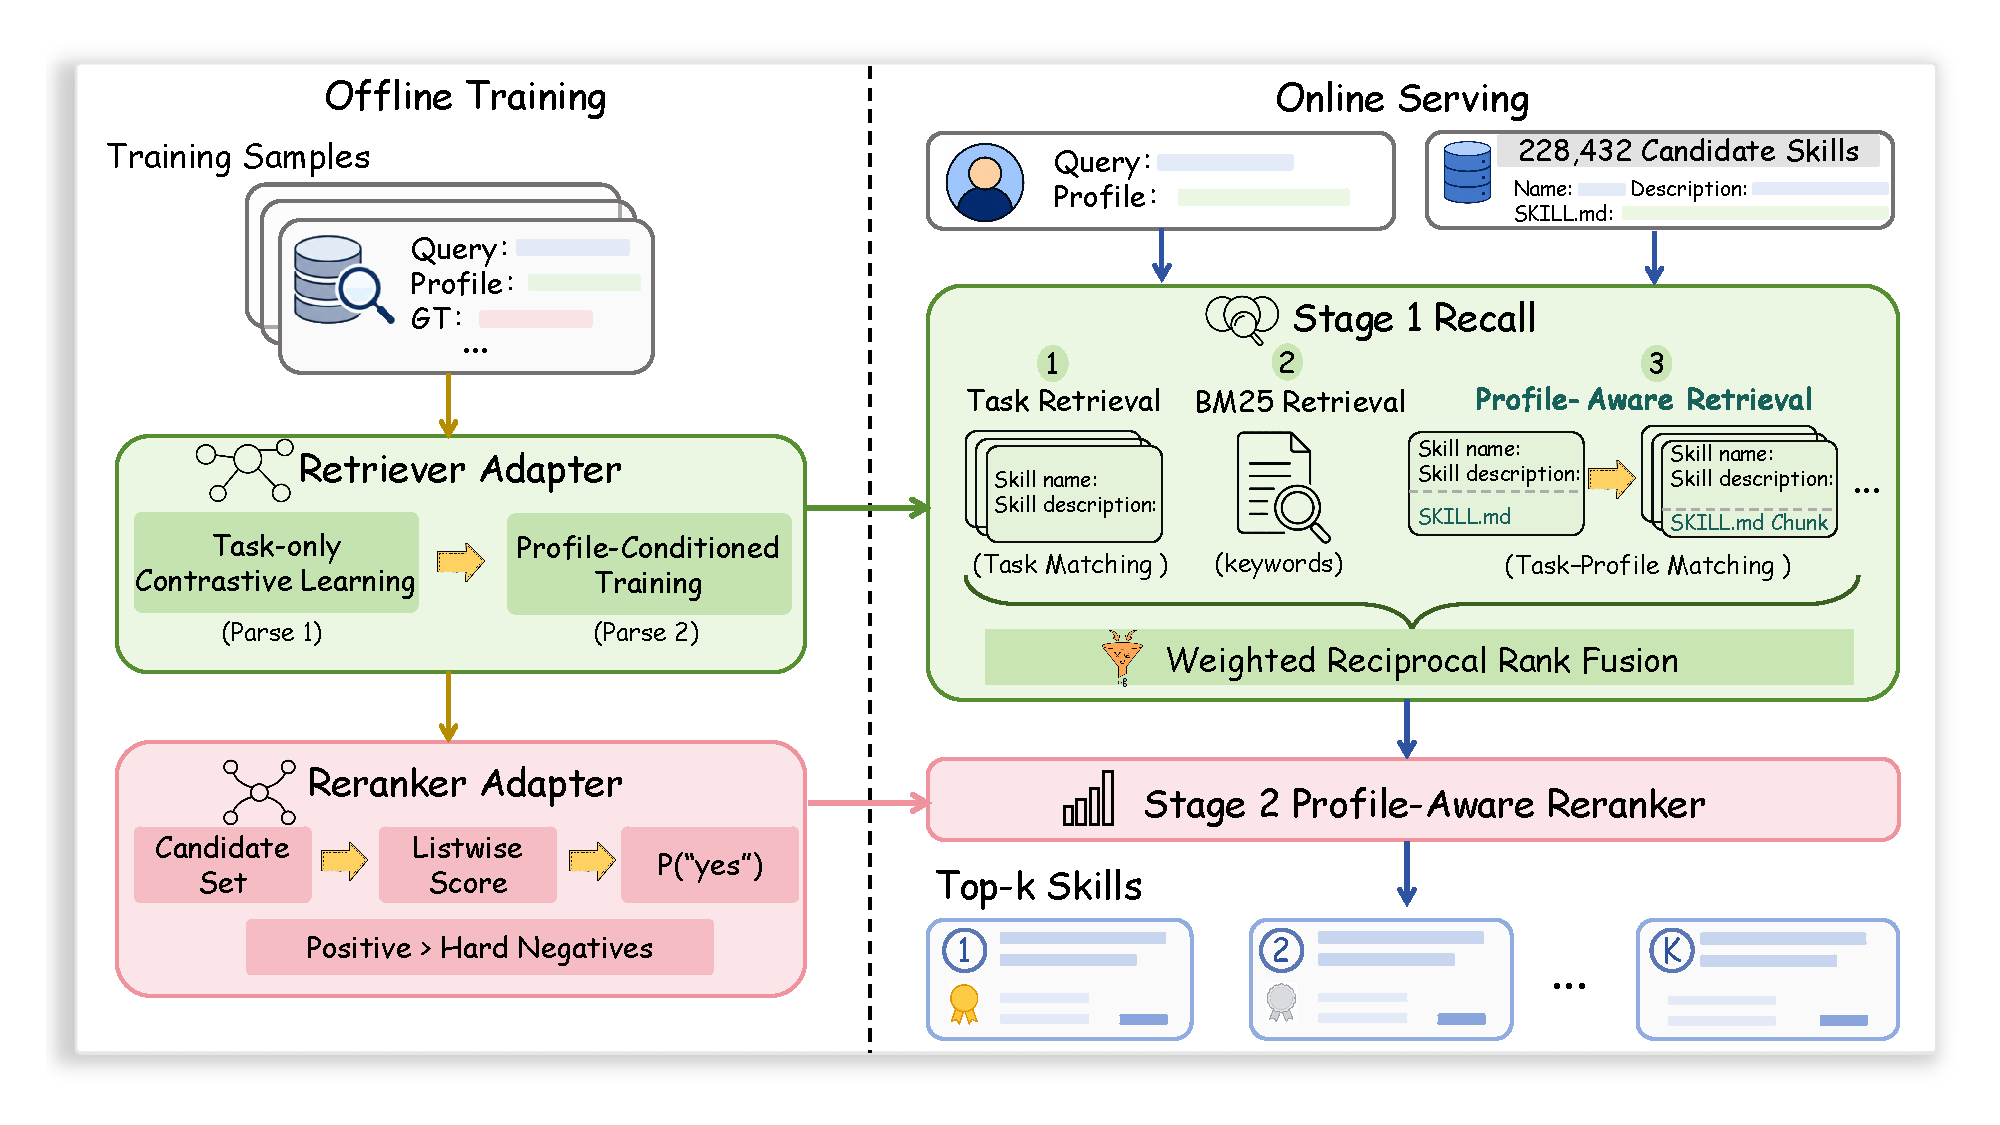
\includegraphics[width=0.98\columnwidth]{Figures/fig2.pdf}
    \caption{Overview of the proposed personalized skill routing framework. During offline training, user profile-aware supervision is constructed to optimize a dense retriever and a reranker. During online serving, the retriever recalls candidate skills from the repository, and the reranker produces the final personalized ranking.}
    \label{fig:method}
\end{figure}





%  现有训练数据集的不足 没有用户信息 缺少基于用户信息的hard negative 同时训练模型的需要 
% 我们基于llm  构建了两阶段训练数据 
% 为了保证数据质量 
% 最后我们使用这些方法 构建了多少训练数据 每条数据对应多少hard negative 



% \subsection{Persona-aware Supervision Construction}
% \label{subsection:Persona-aware Supervision Construction}
% \liu{why this subsection is the part of the method}
% 现有的技能检索数据集\cite{cho2026skillretlargescalebenchmarkskill,su2026skillretrievalaugmentationagentic，li2026skillsbenchbenchmarkingagentskills}都专注与提供任务-技能监督，但它们无法训练基于用户角色的个性化skillrouting。因此，如图 \ref{fig:benchmark}右侧的流程所示，我们构建了用于训练个性化推荐模型的数据集，其中包含明确的基于用户角色的监督和反事实监督。


% High-quality supervision is essential for learning personalized retrieval models. However, existing task--skill datasets are primarily designed for generic retrieval and therefore provide limited supervision for personalized retrieval. Specifically, many task--skill pairs can be matched through superficial lexical overlap, negative samples are often too easy to distinguish, and the resulting supervision does not reflect the influence of user personas on skill preference.

% To construct effective training supervision, we first improve the quality and difficulty of the original task--skill pairs through low-overlap filtering and semantic hard negative mining. Based on the refined data, we then construct two complementary forms of supervision. The first is task-centric supervision, which captures semantic relevance between tasks and skills for retrieval learning. The second is persona counterfactual supervision, which augments the original supervision with persona-dependent preferences by modifying user personas while preserving task semantics. Together, these supervision signals form the final persona-aware training data used to optimize our retrieval model.

% \paragraph{Skill-grounded Task and Persona Generation.}
% % We begin by sampling a target skill $S^{+}$ from the candidate repository. Conditioned on its name, description, and procedural content, an LLM generates a realistic task query $q$ together with a compatible user persona $p$. The generation prompt requires that the task be solvable by $S^{+}$ and that the persona contain decision-relevant attributes, such as language, region, preferred platform, payment method, or other execution constraints. This process establishes a base positive association $(p,q,S^{+})$ without relying on manually authored training queries. To prevent the generated task description from trivially revealing its target skill, we perform low-overlap filtering using a pretrained embedding model. Generated queries whose semantic similarity to any evaluation query exceeds a predefined threshold are removed. 
% We begin by sampling a target skill $S^{+}$ from the candidate repository. Given its name, description, and procedural body, an LLM synthesizes a realistic task query $q$ together with a compatible user persona $p$. The generation prompt constrains $q$ to be solvable by $S^{+}$ and requires $p$ to include routing-relevant attributes, such as language, region, preferred platform, payment method, and other execution constraints. This process yields a base positive triplet $(p,q,S^{+})$.

% % \paragraph{Semantic Hard-Negative Mining.}
% % When mining hard negatives, we account for both persona-aware and task-aware supervision signals. Given the generated positive triples $(p,q,S^{+})$, we mine hard negatives to strengthen the training signal. For task-centric supervision, we retrieve semantically similar skills via an embedding model and also include the annotated hard negatives provided with the data. For persona-conditioned supervision, we expand retrieval to 100 candidates and employ an LLM judge to evaluate each against both the task and the persona, prioritizing instances where high embedding similarity conflicts with the LLM's assessment of persona incompatibility; these candidates are ranked by a combined score. To mitigate false negatives, we apply a unified filtering stage: we discard candidates with task similarity above 0.9 and no persona conflict to avoid penalizing valid alternatives, remove those whose skill names overlap the ground truth by more than 60\%, and exclude entries lacking valid skill content. This yields a structured training instance $(p,q,S^{+},S^{-})$, where $S^{-}$denotes the curated set of hard negatives, ready for the subsequent learning objective.

% \paragraph{Semantic Hard-Negative Mining.}
% For each constructed positive triplet $(p,q,S^{+})$, we curate hard negatives using complementary task-centric and persona-conditioned supervision signals. For task-centric supervision, an embedding model retrieves semantically similar skills, which are combined with the annotated hard negatives from the source data. For persona-conditioned supervision, we retrieve the top-100 candidates from the full skill repository and use an LLM-based judge to assess each candidate in terms of both task relevance and persona compatibility. We prioritize candidates that are semantically similar to the query yet incompatible with the persona-specific constraints.The resulting supervision is represented as
% $\left(p,q,S^{+},\mathcal{S}^{-}\right)$,where $\mathcal{S}^{-}$ denotes the curated set of hard negatives.



% \paragraph{Persona Counterfactual Augmentation.}

% To further strengthen the persona-conditioned supervision signals, we adopt a Persona Counterfactual Augmentation strategy similar to that used in the benchmark construction. Unlike the persona-first benchmark procedure, which modifies the persona before re-annotating the optimal skill, the training procedure follows a target-first design: it selects a curated hard negative as the new target and generates a counterfactual persona under which that skill is preferred.
% Given $(p,q,S^{+},\mathcal{S}^{-})$, we select a curated hard negative $\tilde{S}^{+}\in\mathcal{S}^{-}$ as the counterfactual target and prompt an LLM to generate a persona $\tilde{p}$ under which $\tilde{S}^{+}$ is preferred. The original target $S^{+}$ is then included in the new negative set:
% $\left(\tilde{p},q,\tilde{S}^{+},\tilde{\mathcal{S}}^{-}\right).$ This construction provides direct contrastive supervision for learning how persona changes alter the preferred skill under the same task.

% To reduce false negatives, we apply a unified filtering stage that removes: (i) candidates with a task-similarity score above $0.9$ and no identified persona conflict, as they are likely to be valid alternatives; (ii) candidates whose skill names have more than $60\%$ string overlap with the ground-truth skill name, as they may be duplicates or near-equivalent skills; and (iii) candidates without valid skill-body content. 

% The final dataset contains 2,712 task-centric and 7,459 persona-conditioned instances, jointly supervising task relevance and persona-specific skill preference.Representative examples are shown in Table~\ref{tab:training_examples_persona}.



% \paragraph{Semantic Hard Negative Mining.}
% Randomly sampled negative skills are often semantically unrelated to the query, providing limited training signals. Instead, for each task, we retrieve the top-$K$ most similar skills from the entire skill repository using a pretrained embedding model. After removing the annotated positive skill, the remaining candidates are treated as hard negatives. These negatives are semantically close to the target skill, forcing the retriever to learn fine-grained semantic discrimination rather than coarse relevance matching.

% Based on the filtered positives and mined hard negatives, we obtain the task-centric supervision tuple

% \[
% (q, s^{+}, \mathcal{S}^{-}),
% \]

% where $q$ denotes the task query, $s^{+}$ is the ground-truth skill, and $\mathcal{S}^{-}$ represents the corresponding hard negative skills.



% Existing task-skill datasets are designed for generic skill retrieval and typically consist only of user requests paired with their target skills. Such supervision is insufficient for persona-conditioned retrieval for two reasons. First, the absence of explicit user persona information prevents the retriever from learning persona-aware semantic representations. Second, existing datasets provide only positive task-skill pairs, lacking persona-aware hard negatives that are essential for training a fine-grained reranker to distinguish semantically similar candidate skills.

% To address these limitations, we automatically construct a two-stage persona-aware supervision corpus using a large language model (LLM). Given the original dataset

% \begin{equation}
% \mathcal{D}=\{(Q_i,S_i)\}_{i=1}^{N},
% \end{equation}

% where $Q_i$ denotes a user request and $S_i$ is the corresponding target skill, we transform each sample into two complementary supervision datasets tailored for the two-stage retrieval framework,

% \begin{equation}
% \mathcal{D}^{\text{ret}}
% =
% \{(Q_i,P_i,S_i)\}_{i=1}^{N},
% \end{equation}

% \begin{equation}
% \mathcal{D}^{\text{rank}}
% =
% \{(Q_i,P_i,S_i,\mathcal{H}_i)\}_{i=1}^{N},
% \end{equation}

% where $P_i$ denotes the inferred user persona and $\mathcal{H}_i$ is a set of persona-aware hard negative skills. The retrieval supervision equips the embedding model with persona-aware semantic representations, while the ranking supervision enables the reranker to discriminate among semantically similar candidate skills according to user personas.

% As illustrated in Figure~\ref{fig:method}, the supervision corpus is constructed in two sequential stages. In the first stage, the LLM infers a persona profile from each user request and pairs it with the corresponding target skill to construct the retrieval supervision dataset $\mathcal{D}^{\text{ret}}$. In the second stage, the retriever trained on $\mathcal{D}^{\text{ret}}$ is used to retrieve top-ranked candidate skills. Based on these candidates, the LLM further identifies persona-confusable skills and constructs persona-aware hard negatives, yielding the ranking supervision dataset $\mathcal{D}^{\text{rank}}$. Consequently, the second-stage supervision is built upon the retrieval capability learned in the first stage, ensuring that the generated hard negatives are both semantically relevant and persona-sensitive.

% To ensure annotation quality, all generated samples are required to satisfy predefined structural constraints. Samples with incomplete persona annotations, inconsistent hard negatives, or malformed outputs are automatically discarded and regenerated. This automatic construction pipeline produces high-quality supervision for both retriever and reranker training without requiring manual annotation.

% //

% Training persona-conditioned retrieval models requires supervision that captures the relationship between user requests, user personas, and target skills. However, existing datasets typically provide only task descriptions and their corresponding skills, without explicit persona information. Consequently, they cannot directly su\%ort learning persona-conditioned retrieval.
% \textcolor{red}{reference}

% To address this limitation, we automatically construct persona-aware supervision using a large language model (LLM). Let the original dataset be

% \begin{equation}
% \mathcal{D}=\{(Q_i,S_i)\}_{i=1}^{N},
% \end{equation}

% where $Q_i$ denotes a user request and $S_i$ is the corresponding target skill. For each sample, the LLM augments the original task-skill pair with persona-aware annotations and transforms it into

% \begin{equation}
% \mathcal{S}_i=(Q_i,P_i,E_i,T_i,S_i^{+}),
% \end{equation}

% where $P_i$ denotes the inferred user persona, $E_i$ represents su\%orting evidence extracted from the request, $T_i$ is a reasoning trajectory explaining how the persona influences skill selection, and $S_i^{+}$ is the target skill. The resulting supervision provides structured persona information for subsequent retriever and reranker learning.

% We employ a structured prompting pipeline consisting of four sequential stages. Given a user request $Q$, the LLM first infers a persona profile by identifying stable user characteristics implied by the request. It then generates su\%orting evidence to justify each inferred persona attribute. Based on the generated persona and evidence, the LLM produces an explicit reasoning trajectory describing how persona information affects skill selection. Finally, it verifies the consistency between the generated annotations and the target skill, yielding a unified supervision schema for all training samples.

% To improve annotation quality, all generated samples are required to satisfy a predefined structured output format. Samples with missing fields, inconsistent persona annotations, unsu\%orted reasoning, or malformed outputs are automatically discarded and regenerated. This automatic annotation pipeline produces high-quality persona-aware supervision without requiring manual annotation.


\subsection{Learning Profile-Conditioned Routing}
% \liu{I have provided a version here that can replace the subsection "User Profile-aware Retrieval Model Learning". You can further supplement and modify this version.}

\paragraph{Counterfactual Supervision.}
% Existing skill retrieval datasets such as SkillRet\cite{cho2026skillretlargescalebenchmarkskill}, SkillsBench \cite{li2026skillsbenchbenchmarkingagentskills} SWE-Skills\cite{han2026sweskillsbenchagentskillsactually} and SRA \cite{su2026skillretrievalaugmentationagentic} are valuable for general skill retrieval, but they are insufficient for modeling personalized skill routing. To address this limitation, as illustrated in the right-hand flow of Figure~\ref{fig:benchmark}, a dataset is constructed specifically for training personalized recommendation models, incorporating both explicit persona-based supervision and counterfactual supervision.

Existing skill retrieval datasets such as SkillRet~\cite{cho2026skillretlargescalebenchmarkskill}, SkillsBench~\cite{li2026skillsbenchbenchmarkingagentskills}, SWE-Skills~\cite{han2026sweskillsbenchagentskillsactually}, and SRA~\cite{su2026skillretrievalaugmentationagentic} provide task--skill pairs, but cannot specify when a profile should overturn an otherwise plausible task-only match. We therefore construct training supervision around task-fixed counterfactual pairs (illustrated in Figure~\ref{fig:benchmark}), separately from the held-out benchmark. Starting from a target skill $S^{+}$, we generate a task $q$ and a compatible profile $p$, then mine task-relevant skills that conflict with $p$ through retrieval and verification as hard negatives set $S^{-}$. For one such skill $\tilde{S}^{+} \in S^{-}$ , we generate a counterfactual profile $\tilde{p}$ under which it becomes the preferred skill for the same $q$ and subsequently mine a corresponding set of hard negatives  $\tilde{S}^{-}$. The resulting paired tuples $(p, q, S^{+}, S^{-})$ and $(\tilde{p}, q, \tilde{S}^{+}, \tilde{S}^{-})$ therefore differ only in the routing-relevant profile but require different rankings. They directly supervise the desired reversal: profile information must discriminate between functionally plausible skills, rather than merely accompany task wording. We remove likely valid alternatives, near duplicates, and invalid skill files to limit false negatives; the resulting corpus contains 2,712 task-centric and 7,459 profile-conditioned instances, with examples in Appendix Table~\ref{tab:training_examples_persona}.

\paragraph{Two-Phase Retriever Training.}
We adapt Qwen3-Embedding-0.6B and Qwen3-Reranker-0.6B~\cite{qwen3embedding} to complementary stages of routing. The retriever operates over the full repository, where a missed functionally relevant skill cannot be recovered, whereas the reranker receives only task-relevant alternatives and can focus on their profile-conditioned differences. Pretrained embeddings capture general semantic similarity rather than skill-specific capability matching. We consequently train the retriever progressively. Phase~1 uses task-only queries and hard negatives to establish routing-specific task--skill alignment. Phase~2 adds profile constraints and the counterfactual pairs above, making the profile a discriminative signal among functionally plausible skills rather than a shortcut for weak task matching. Both phases use InfoNCE~\cite{oord2019representationlearningcontrastivepredictive} over the reference skill, curated hard negatives, and in-batch negatives.


% We adopt a two-phase optimization strategy for the dense retriever. Directly training on persona-conditioned queries risks the model
% overfitting to explicit persona attributes while underlearning the fundamental task--skill semantic
% relationships that form the basis of effective retrieval. A progressive training schedule mitigates this by first establishing strong
% semantic alignment and then layering persona-aware discrimination on top.

% In the first phase, the retriever is trained with task-only queries containing no persona information. Each query presents the task name,
% description, and core requirements, paired with the ground-truth skill as the positive document and embedding-based hard negatives. This
% teaches the model to match tasks to skills based on functional relevance alone. In the second phase, persona constraints—country, language,
% domain, and other user-context factors—are a\%ended to the query. The training data is augmented with persona counterfactual samples: for
% the same task, different persona specifications yield different ground-truth skills, and these become mutual negatives. This teaches the
% retriever that persona can flip the correct skill for an otherwise identical task.

% This two-phase a\%roach yields a retriever that retains strong semantic matching while gaining personalization sensitivity.with the gain concentrated on
% persona-sensitive queries where context-dependent skill disambiguation is required.

% Each training instance contains one positive skill and multiple hard negatives mined from the skill repository. Since these negatives are semantically similar to the target skill and often differ only in persona compatibility, retrieval naturally becomes a contrastive ranking problem. We therefore optimize the retriever using the InfoNCE objective:

% % \begin{equation}
% % \mathcal{L}_{\text{InfoNCE}}
% % =
% % -
% % \log
% % \frac{
% % \exp(\mathrm{sim}(q,s^{+})/\tau)
% % }
% % {
% % \exp(\mathrm{sim}(q,s^{+})/\tau)
% % +
% % \sum_{j=1}^{K}
% % \exp(\mathrm{sim}(q,s_j^{-})/\tau)
% % },
% % \end{equation}

% \begin{equation}
% \mathcal{L}_{\text{InfoNCE}}
% =
% -\log
% \frac{
% \exp(\mathrm{sim}(q,s^{+})/\tau)
% }{
% \sum\limits_{s\in\{s^{+}\}\cup\mathcal{N}}
% \exp(\mathrm{sim}(q,s)/\tau)
% },
% \end{equation}

% where $s^{+}$ denotes the positive skill, $\mathcal{N}$ denotes the set of hard negative skills mined for the query, $\mathrm{sim}(\cdot,\cdot)$ represents cosine similarity between query and skill embeddings, and $\tau$ is a temperature parameter.

% We fine-tune the retriever end-to-end on 2$\times$A100 GPUs with per-device batch size 1 and gradient accumulation over 16 steps, yielding
% an effective batch of 16 query--candidate groups per update. Training runs for 3 epochs with a maximum sequence length of 2048 under
% DeepSpeed ZeRO-2.

\paragraph{Profile-Aware Reranker Training.}
Unlike the retriever, the reranker is trained directly on profile-conditioned candidate groups. Each group contains one target and task-relevant but profile-conflicting hard negatives; candidates include their names, descriptions, and procedural bodies. We optimize a listwise objective~\cite{10.1145/1390156.1390306} using the model's \textit{yes} logit as the relevance score. This objective reflects the final routing decision: the suitable skill must outrank near misses that satisfy the task in isolation but violate a profile constraint. Complete objectives are provided in Appendix~\ref{app:training_objectives}.

% We employ Qwen3-Reranker as a generative relevance judge. Given an instruction, a query, and a candidate skill, the model assesses whether the candidate satisfies the query, and its logit for the token \textit{yes} is used as the relevance score $r_{\phi}(u,S)$. The reranker is optimized with a listwise objective \cite{10.1145/1390156.1390306}:
% \begin{equation}
% \mathcal{L}_{\mathrm{rank}}
% =
% -\frac{1}{B}
% \sum_{i=1}^{B}
% \log
% \frac{
% \exp\!\left(
% r_{\phi}(u_i,S_i^{+})/\tau_{\mathrm{rank}}
% \right)
% }{
% \sum\limits_{S\in\{S_i^{+}\}\cup\mathcal{N}_i}
% \exp\!\left(
% r_{\phi}(u_i,S)/\tau_{\mathrm{rank}}
% \right)
% },
% \end{equation}
% where $\tau_{\mathrm{rank}}$ is the ranking temperature. By normalizing scores within each candidate group, the objective directly encourages the user profile-compatible target skill to outrank semantically similar alternatives.



% Unlike the retriever, the reranker operates on a small candidate set that is already semantically relevant to the task. Its role is therefore not broad semantic matching but final persona-conditioned discrimination. Given a query containing the task and persona constraints, we form a ranking group from the retriever outputs with one positive skill and multiple hard negatives. 

% As a result, personalized skill recommendation naturally becomes a relative ranking problem rather than an independent binary classification problem. We therefore adopt a listwise ranking objective:
% \begin{equation}
% \mathcal{L}_{\text{rank}}
% =
% -
% \log
% \frac{
% \exp(r^{+}/\tau)
% }
% {
% \sum_{i=1}^{N}
% \exp(r_i/\tau)
% },
% \end{equation}
% where $r^{+}$ denotes the relevance score assigned to the target skill, $\{r_i\}_{i=1}^{N}$ are the scores of all candidates within the ranking group, and $\tau$ is a temperature parameter.

% We fine-tune the reranker on 1$\times$A100 with batch size 4 and gradient accumulation over 4 steps, matching the same effective
% batch size of 16. Training runs for 3 epochs with a cosine learning rate schedule and 10\% warmup.

\subsection{Profile-Aware Skill Routing}
\label{subsection:two_stage_inference}

Task relevance alone does not establish profile compatibility. Although two skills may expose the same high-level capability, the conditions that make one appropriate for a particular user often differ significantly. For example, required inputs, supported platforms, output formats, dependencies, and exceptions are often stated only in their procedural bodies. SkillFeed therefore performs \emph{profile-aware skill-body retrieval}: it retrieves localized, profile-relevant conditions from skill body for a task--profile query and converts the retrieved chunks into a skill-level compatibility signal. The signal complements, rather than replaces, task relevance: it identifies which task-relevant skills state execution conditions that fit the requesting profile.

% \liu{The "\texttt{SKILL. md} Chunk Index" section is a bit verbose, so merge it into the Candidate Recall paragraph}
\paragraph{Structured Skill-Body Representation.}
Skill descriptions are concise summaries of core functionality~\cite{openai2026skills}, whereas profile-relevant conditions are distributed across sections such as \textit{When to use}, \textit{Inputs}, \textit{Examples}, \textit{Constraints}, and \textit{Dependencies}. Encoding an entire skill as one document would mix these conditions with unrelated capabilities and dilute a decisive local match. We instead split each file into Markdown-structured chunks, following passage-level retrieval~\citep{lewis2020rag}, and encode them independently. Each chunk retains its skill name, description, section path, and content; long sections are divided into overlapping passages. This representation turns an implicit document-level judgment into retrievable evidence: a profile constraint can match the precise passage that supports or rules out a skill.

% For each chunk, we preserve its skill identity and section path:
% \[
% \begin{aligned}
% &\texttt{Skill: name}\\
% &\texttt{Description: description}\\
% &\texttt{Section: path}\\
% &\texttt{Content: chunk}.
% \end{aligned}
% \]

\paragraph{Evidence Aggregation.}
For a task--profile query, profile-aware skill-body retrieval returns matching chunks, which we aggregate into a skill-level compatibility score.
For each candidate skill $S_i$, let $\mathcal{C}_{S_i}$ denote the set of
retrieved chunks belonging to $S_i$, and let $h_c$ denote the dense similarity
score of chunk $c$.
Let $\operatorname{TopM}(\mathcal{C}_{S_i})$ denote the set of the $M$
highest-scoring chunks in $\mathcal{C}_{S_i}$. The aggregated score is
computed as 
\begin{equation}
\begin{aligned}
\operatorname{score}(S_i)
={}&
\alpha
\max_{c\in\mathcal{C}_{S_i}} h_c
+
\frac{\beta}{M}
\sum_{c\in\operatorname{TopM}(\mathcal{C}_{S_i})} h_c \\
&+
\gamma
\log\!\left(1+\left|\mathcal{C}_{S_i}\right|\right),
\end{aligned}
\label{eq:chunk_to_skill_aggregation}
\end{equation}
where $\alpha$, $\beta$, and $\gamma$ are non-negative aggregation weights, and $M$ is the number of highest-scoring chunks included in the mean term. The maximum term preserves a single decisive condition, the top-$M$ mean distinguishes repeated evidence from an isolated noisy passage, and the logarithmic count only mildly rewards multiple supporting chunks. This converts local passages into a compatibility signal without mechanically favoring longer skill files.

\paragraph{Integrating Evidence into Routing.}
Profile-aware skill-body retrieval is combined with one profile signal and two task signals: profile dense over profile, task dense retrieval over skill, and BM25 ~\citep{robertson2009bm25} over the same text. The latter preserves exact lexical matches, such as tool names, platforms, and file formats that dense representations may underweight. We combine the three ranked lists with weighted reciprocal rank fusion~\citep{cormack2009rrf}, which avoids calibrating heterogeneous raw scores. The reranker then receives the task, profile, and complete skill information to resolve any remaining conflicts. Thus, task-level retrieval establishes functional plausibility, while profile-aware skill-body retrieval exposes the local conditions needed to choose among plausible skills.

\begin{table*}[!t]
\centering
\resizebox{\linewidth}{!}{%
\begin{tabular}{l c c c c c}
\toprule
\textbf{Method}
& \textbf{Input}
% & \textbf{Reranker Input}
& \textbf{All Hit@1}
& \textbf{Sensitive Hit@1}
& \textbf{Insensitive Hit@1}
& \textbf{CF-Switch Acc.} \\
% & \textbf{MRR@20}
% & \textbf{nDCG@20} \\
\midrule

Qwen3-Emb-0.6B + Qwen3-Reranker-0.6B
& Task + Profile
% & Task
& 0.520
& 0.426
& 0.611
& 0.143 \\
% & 0.622
% & 0.672 \\

SkillFeed Emb Phase 1
& Task
% & --
& 0.483
& 0.340
& 0.623
& 0.052 \\
% & 0.583
% & 0.642 \\

SkillFeed Emb Phase 2
& Task + Profile
% & --
& 0.617
& 0.512
& 0.719
& 0.286 \\
% & 0.697
% & 0.741 \\

SkillFeed Emb Phase 2 + SkillFeed Reranker
& Task
% & Task
& 0.644
& 0.444
& 0.838
& 0.026 \\
% & 0.712
% & 0.749 \\

SkillFeed Emb Phase 2 + SkillFeed Reranker
& Task + Profile
% & Task + Profile
& \textbf{0.733}
& \textbf{0.630}
& \textbf{0.832}
& \textbf{0.377} \\
% & \textbf{0.788}
% & \textbf{0.819} \\

\bottomrule
\end{tabular}%
}
\caption{Effect of profile conditioning at the retrieval and reranking stages. ``Task'' denotes task-only conditioning, whereas ``Task + Profile'' denotes
profile-aware conditioning. All metrics are computed on 329 test samples,
162 profile-sensitive
samples and 167
profile-insensitive queries.
CF-Switch Acc. denotes Hit@1 on 77 profile-counterfactual samples.}
\label{tab:personalization_matter}
\end{table*}



% Main Results Table - Corrected Version
\begin{table*}[!h]
\centering
\small
\setlength{\tabcolsep}{5pt}
\renewcommand{\arraystretch}{1.08}

% \resizebox{\textwidth}{!}{%
\begin{tabular}{@{}l l c c c c c c@{}}
\toprule
\textbf{Embedding Model}
& \textbf{Reranker Model}
& \textbf{Hit@1}
& \textbf{Hit@3}
& \textbf{Hit@5}
& \textbf{Hit@10}
& \textbf{MRR@20}
& \textbf{nDCG@20} \\
\midrule

\multicolumn{8}{@{}l}{\textit{(1) Embedding Only (No Reranker)}} \\
\addlinespace[2pt]

BM25 Only
& ---
& 0.410 & 0.538 & 0.578 & 0.611 & 0.485 & 0.528 \\

E5-large-v2
& ---
& 0.322 & 0.474 & 0.508 & 0.565 & 0.410 & 0.459 \\

BGE-large-en-v1.5
& ---
& 0.386 & 0.492 & 0.556 & 0.626 & 0.461 & 0.509 \\

Qwen3-Emb-0.6B
& ---
& 0.416 & 0.559 & 0.644 & 0.717 & 0.514 & 0.575 \\

SkillFeed Emb Phase 1 (Task-only FT)
& ---
& 0.483 & 0.638 & 0.699 & 0.787 & 0.583 & 0.642 \\

Qwen3-Emb-8B
& ---
& 0.471 & 0.574 & 0.634 & 0.724 & 0.574 & 0.634 \\

SkillFeed Emb Phase 2 (User profile FT)
& ---
& \textbf{0.617}
& \textbf{0.754}
& \textbf{0.796}
& \underline{0.833}
& \textbf{0.697}
& \textbf{0.741} \\

BM25 + Task Dense + Profile Dense
& ---
& 0.492 & 0.641 & 0.705 & 0.815 & 0.597 & 0.663 \\

BM25 + Task Dense + Profile Chunk Dense
& ---
& \underline{0.517}
& \underline{0.705}
& \underline{0.775}
& \textbf{0.860}
& \underline{0.632}
& \underline{0.698} \\

\addlinespace[3pt]
\midrule
\multicolumn{8}{@{}l}{\textit{(2) Embedding + Reranker}} \\
\addlinespace[2pt]

SkillFeed Emb Phase 2
& Qwen3-Reranker-0.6B
& 0.559
& 0.757
& 0.818
& \underline{0.882}
& 0.668
& 0.727 \\

SkillFeed Emb Phase 2
& BGE-reranker-v2-m3
& 0.304
& 0.495
& 0.596
& 0.702
& 0.434
& 0.525 \\

SkillFeed Emb Phase 2
& Qwen3-Reranker-8B
& \underline{0.632}
& \underline{0.772}
& \underline{0.821}
& 0.881
& \underline{0.717}
& \underline{0.763} \\

SkillFeed Emb Phase 2
& LLM (mimo-v2.5-pro)
& 0.590
& 0.726
& 0.769
& 0.824
& 0.672
& 0.715 \\

Qwen3-Emb-8B
& Qwen3-Reranker-8B
& 0.602
& 0.723
& 0.787
& 0.836
& 0.681
& 0.724 \\

SkillRouter Emb 0.6B
& SkillRouter Reranker 0.6B
& 0.614
& 0.726
& 0.751
& 0.772
& 0.675
& 0.703 \\

SkillFeed Emb Phase 2
& SkillFeed Reranker
& \textbf{0.733}
& \textbf{0.818}
& \textbf{0.863}
& \textbf{0.891}
& \textbf{0.788}
& \textbf{0.819} \\

\addlinespace[3pt]
\midrule
\multicolumn{8}{@{}l}{\textit{(3) Full Pipeline (BM25 + Dense + Reranker)}} \\
\addlinespace[2pt]

BM25 + Task Dense + Profile Dense
& SkillFeed Reranker
& \textbf{0.751}
& \underline{0.836}
& \underline{0.869}
& \underline{0.900}
& \textbf{0.803}
& \underline{0.831} \\

BM25 + Task Dense + Profile Chunk Dense
& SkillFeed Reranker
& \underline{0.739}
& \textbf{0.851}
& \textbf{0.888}
& \textbf{0.918}
& \textbf{0.803}
& \textbf{0.838} \\

\bottomrule
\end{tabular}%
% }
\caption[Main results on SkillFeed-Bench.]{
Main results on SkillFeed-Bench.
We organize results by pipeline stage:
(1) Embedding Only,
(2) Embedding + Reranker, and
(3) Full Pipeline.
Bold indicates the best result, and
\underline{underlining} indicates the second-best result.
Task/Profile Dense use SkillFeed Emb Phase 2 for respective inputs; Profile Chunk Dense chunks input.
}
\label{tab:main_results}
\end{table*}

\section{Experiment}

We evaluate three questions. First, does profile conditioning improve routing precisely when a profile changes the suitable skill? Second, how does SkillFeed compare with general-purpose, skill-specific, and larger pretrained retrieval and reranking models? Third, do its retrieval, reranking, and profile-aware skill-body components make complementary contributions? 
Unless otherwise stated, all results are evaluated on SkillFeed-Bench.

% \begin{table*}[!t]
% \centering
% \caption[Effect of persona conditioning.]{Effect of persona conditioning. Placeholder table for the core comparison between task-only and persona-aware routing.}
% \label{tab:personalization_matter}
% \resizebox{\linewidth}{!}{
% \begin{tabular}{l c c c c c c}
% \toprule
% \textbf{Method} & \textbf{All Hit@1} & \textbf{Sensitive Hit@1} & \textbf{Insensitive Hit@1} & \textbf{CF-Switch Acc.} & \textbf{MRR@20} & \textbf{nDCG@20} \\
% \midrule
% Task-only baseline & -- & -- & -- & -- & -- & -- \\
% % Persona-aware baseline & -- & -- & -- & -- & -- & -- \\
% Phase 1 retriever & -- & -- & -- & -- & -- & -- \\
% Phase 2 retriever & -- & -- & -- & -- & -- & -- \\
% Phase 2 + reranker w/o persona & -- & -- & -- & -- & -- & -- \\
% Phase 2 + reranker w/ persona & -- & -- & -- & -- & -- & -- \\
% \bottomrule
% \end{tabular}
% }
% \end{table*}


\subsection{Experimental Setup}
SkillFeed is initialized from Qwen3-Embedding-0.6B for retrieval and Qwen3-Reranker-0.6B for reranking. We evaluate both a skill-level profile-conditioned dense channel and the proposed profile-aware skill-body retrieval channel; each can be fused with task-oriented dense retrieval and BM25 before reranking. Unless otherwise stated, the system reranks the top 50 fused candidates. Complete training, preprocessing, and inference settings are provided in Appendix~\ref{app:implementation_details}.

\paragraph{Evaluation Protocol.}

We report Hit@K for $K\in\{1,3,5,10\}$, MRR@20, and nDCG@20. Hit@K measures whether the annotated skill is surfaced within the top $K$ results, whereas MRR@20 and nDCG@20 emphasize its early-rank position. To evaluate profile sensitivity, we report results both on the full benchmark and on 162 profile-sensitive queries with  user context constraints. We also refer to Hit@1 on its 77 profile-counterfactual subset as counterfactual-switch accuracy (CF-Switch Acc.).



\paragraph{Baselines.}

We compare SkillFeed with retrieval and reranking baselines corresponding to the two stages of our pipeline.

\textit{Retrievers.}
We include BM25 \cite{robertson2009bm25} as a sparse lexical baseline. E5-large-v2~\cite{wang2022e5} and BGE-large-en-v1.5~\cite{bge_embedding} represent general-purpose dense retrievers. We further evaluate the dense retriever from SkillRouter~\cite{zheng2026skillrouter}, which is specifically trained for task-to-skill routing. Qwen3-Embedding-8B~\cite{qwen3embedding} is included without task-specific adaptation to examine whether model scale alone can replace routing-specific supervision. Finally, we report our Phase~1 retriever to isolate the effect of profile-conditioned adaptation.

\textit{Rerankers.}
We compare our reranker against the pretrained Qwen3-Reranker-0.6B~\cite{qwen3embedding}, BGE-reranker-v2-m3~\cite{chen2024bge}, and the pretrained Qwen3-Reranker-8B~\cite{qwen3embedding}. We additionally use MiMo-V2.5-Pro~\cite{mimo2026v25pro} as LLM reranker, prompting it to assess each candidate with respect to both the task requirements and the profile constraints.

All retrievers search the same 228K-skill repository. For reranker comparisons, every model reranks the same fixed candidate lists, so differences can be attributed to candidate discrimination rather than to recall coverage.


% \subsection{Experimental Setup}
% %  我们的所有实验都在我们的benchmark进行
% We evaluate the effectiveness of our user profile-aware retrieval framework on SkillFeed-Bench, focusing on both dense retrieval and cross-encoder reranking performance under personalized skill recommendation settings.

% We evaluate SkillFeed on SkillFeed-Bench using a dense retriever initialized
% from Qwen3-Embedding-0.6B and a reranker initialized from
% Qwen3-Reranker-0.6B. The default pipeline combines dense,
% BM25, and \texttt{SKILL.md} chunk retrieval and reranks the top 50 fused candidates. Appendix~\ref{app:implementation_details} provides the complete training, preprocessing, and inference settings.

% % The SkillFeed dense retriever is initialized from Qwen3-Embedding-0.6B, and the SkillFeed reranker is initialized from Qwen3-Reranker-0.6B.
% % Both models are fine-tuned on 2$\times$A100 GPUs using AdamW with a learning rate of $1\times10^{-5}$, an effective batch size of 16, a maximum sequence length of 2048, and 3 training epochs.
% % The retriever is trained in two phases: 2,712 task-centric instances are used for task-only alignment, and 7,459 user profile-conditioned instances are used for user profile-aware adaptation.
% % Lexical-overlap filtering uses a threshold of 0.50.
% % For \texttt{SKILL.md} chunk retrieval, Markdown sections are split into passages with a target length of 200--500 tokens, a maximum length of 800 tokens, and a small overlap for continuity.
% % Chunk-to-skill aggregation uses $\alpha=0.70$, $\beta=0.25$, $\gamma=0.05$, and $M=3$.
% % Weighted reciprocal rank fusion uses weights of 0.40 for task dense retrieval, 0.40 for persona dense retrieval over SKILL.md chunks, and 0.20 for BM25.
% % Unless otherwise stated, the full pipeline reranks the top 50 fused candidates; the top-100 setting is evaluated only in the ablation study.

% \subsection{Evaluation Protocol}

% We evaluate retrieval and end-to-end routing performance using Hit@K for $K\in\{1,3,5,10,20,50\}$, Mean Reciprocal Rank (MRR), and NDCG@K.

% % To assess personalization, we report results on both the complete benchmark and a user profile-sensitive subset in which profile variations under the same task induce different ground-truth skills.

% % \subsection{Baselines}

% % We organize baselines into two categories corresponding to the two stages of our pipeline.

% % \paragraph{Dense Retrievers.}
% % We compare against several embedding models of varying scale and domain specificity. E5-large-v2~\citep{wang2022e5} and BGE-large-en~\citep{bge_embedding} represent
% % general-purpose pretrained dense retrievers. SkillRouter~\citep{zheng2026skillrouter} is a skill-specific recommendation system that routes tasks to skill categories. To assess the benefit of
% % domain-specific fine-tuning over model scale, we also evaluate the 8B-parameter pretrained Qwen3-Embedding-8B \cite{qwen3embedding} without any task-specific adaptation. Additionally, we include
% % our Phase~1 retriever (trained with task-only supervision) to isolate the contribution of persona-aware training.

% % \paragraph{Rerankers.}
% % For the reranking stage, we compare against the original pretrained Qwen3-Reranker-0.6B \cite{qwen3embedding} without fine-tuning, BGE-reranker-v2-m3~\citep{chen2024bge} as a cross-encoder baseline, and
% % Qwen3-Reranker-8B\cite{qwen3embedding} to evaluate the effect of model scale. We also report results using mimo-v2.5-pro \cite{mimo2026v25pro} as a zero-shot LLM reranker, which scores each candidate by prompting the
% % model to judge task--skill relevance without any task-specific training.

% % All baselines are evaluated under the same candidate pool of 228,432 skills.

% \subsection{Baselines}

% We compare SkillFeed with retrieval and reranking baselines corresponding to the two stages of our pipeline.

% \paragraph{Retrievers.}
% We include BM25 \cite{bm25} as a sparse lexical baseline. E5-large-v2~\cite{wang2022e5} and BGE-large-en-v1.5~\cite{bge_embedding} represent general-purpose dense retrievers. We further evaluate the dense retriever from SkillRouter~\cite{zheng2026skillrouter}, which is specifically trained for task-to-skill routing. Qwen3-Embedding-8B~\cite{qwen3embedding} is included without task-specific adaptation to examine whether model scale alone can replace routing-specific supervision. Finally, we report our Phase~1 retriever to isolate the effect of profile-conditioned adaptation.

% \paragraph{Rerankers.}
% We compare our reranker against the pretrained Qwen3-Reranker-0.6B~\cite{qwen3embedding}, BGE-reranker-v2-m3~\cite{chen2024bge}, and the pretrained Qwen3-Reranker-8B~\cite{qwen3embedding}. We additionally use MiMo-V2.5-Pro~\cite{mimo2026v25pro} as a zero-shot LLM reranker, prompting it to assess each candidate with respect to both the task requirements and the profile constraints.

% All retrievers search the same skill repository using the same skill-document representation. For reranker comparisons, all models rerank the same candidate lists produced by the fixed retrieval stage, ensuring that differences arise from reranking rather than candidate recall.

\subsection{Main Results}
% Ablation: Pipeline
\begin{table*}[!h]
\small
\centering
% \setlength{\tabcolsep}{1mm}
% \resizebox{\columnwidth}{!}{%
\begin{tabular}{l c c c c}
\toprule
\textbf{Pipeline Configuration} & \textbf{Hit@1} & \textbf{Hit@5} & \textbf{Hit@10} & \textbf{MRR@20} \\
\midrule
\multicolumn{5}{l}{\textit{Single-Stage Retrieval}} \\
BM25 Only & 0.410 & 0.578 & 0.611 & 0.485 \\
SkillFeed Emb Phase 2 & 0.617 & 0.796 & 0.833 & 0.697 \\
\midrule
\multicolumn{5}{l}{\textit{Two-Stage: Dense + Reranker}} \\
SkillFeed Emb Phase 2 + Qwen3-Reranker-0.6B & 0.559 & 0.818 & 0.882 & 0.668 \\
SkillFeed Emb Phase 2 + SkillFeed Reranker & 0.733 & 0.863 & 0.891 & 0.788 \\
\midrule
\multicolumn{5}{l}{\textit{Full Pipeline: BM25 + Dense + Reranker}} \\
Full Pipeline (topk=50) & \textbf{0.751} & \textbf{0.869} & \textbf{0.900} & \textbf{0.803} \\
Full Pipeline (topk=100) & 0.739 & 0.866 & 0.903 & 0.796 \\
\midrule
\multicolumn{5}{l}{\textit{Ablation: Pipeline Components}} \\
Full Pipeline w/o BM25 & 0.723 & 0.878 & 0.909 & 0.788 \\
Full Pipeline w/o Profile Dense & 0.726 & 0.854 & 0.891 & 0.785 \\
\bottomrule
\end{tabular}%
% }
\caption[Ablation on retrieval pipeline.]{Ablation on retrieval pipeline. The full pipeline defaults topk=50. ``w/o'' indicates specific components are removed.}
\label{tab:ablation_pipeline}
\end{table*}
% \liu{You need to add a paragraph to demonstrate the necessity of the person-aware method; here is just a reference}
% \paragraph{Necessity of Personalized Skill Routing.}
% 
% Table~\ref{tab:personalization_matter} presents a controlled comparison between task-only and persona-conditioned routing configurations, evaluated separately on standard and persona-counterfactual queries. The results show that task-only routing is ineffective when the preferred skill changes with persona: the Phase~1 retriever achieves only 0.052 Hit@1 on counterfactual queries, compared with 0.615 on standard queries. Persona-aware training increases counterfactual Hit@1 to 0.286, while persona-conditioned reranking further improves it from 0.026 to 0.377 with only a marginal change on standard queries (0.833 to 0.841). These findings demonstrate that persona conditioning is necessary for routing skills under persona shifts. Table~\ref{tab:main_results} further compares SkillFeed with competitive retrieval and reranking baselines.

\subsubsection{Necessity of Personalized Skill Routing.}
% 这一段想要说明 task center的检索效果不好 没有persona也不能很好的识别这种对于persona senesitive的样例 所以我们提出的问题是实际存在的 benchmark的Persona Counterfactual Augmentation是有效的 基于个性化数据的微调的有效的
% Table~\ref{tab:personalization_matter} presents a controlled comparison between task-only and profile-conditioned routing configurations, The pretrained Qwen baseline and the task-only Phase~1 retriever achieve only 0.143 and 0.052 Hit@1 on profile-counterfactual queries, despite obtaining 0.635 and 0.615 on standard queries. This substantial gap demonstrates that task semantics alone are insufficient for personalized skill routing and confirms the need for profile-counterfactual evaluation. Incorporating the constructed profile-aware supervision in Phase~2 improves counterfactual Hit@1 from 0.052 to 0.286. Moreover, adding user profile conditioning to the reranker further increases counterfactual Hit@1 from 0.026 to 0.377, while standard-query performance changes only marginally from 0.833 to 0.841. These findings demonstrate that personalized skill routing is necessary under profile shifts: the counterfactual construction in SkillFeed-Bench exposes skill changes that task-level evaluation overlooks, while fine-tuning the retriever and reranker on profile-aware data with counterfactual supervision enables them to effectively recognize and resolve these changes.
Table~\ref{tab:personalization_matter} presents a controlled comparison between task-only and profile-conditioned routing configurations. The pretrained Qwen baseline and the task-only Phase~1 retriever achieve only 0.143 and 0.052 Hit@1 on profile-counterfactual queries, despite obtaining 0.611 and 0.623 on profile-insensitive queries. This substantial gap demonstrates that task semantics alone are insufficient for personalized skill routing and confirms the need for profile-counterfactual evaluation. Incorporating the constructed profile-aware supervision in Phase~2 improves counterfactual Hit@1 from 0.052 to 0.286. Moreover, adding user profile conditioning to the reranker further increases counterfactual Hit@1 from 0.026 to 0.377, while insensitive-query performance changes only marginally from 0.838 to 0.832. These findings demonstrate that personalized skill routing is necessary under profile shifts: the counterfactual construction in SkillFeed-Bench exposes skill changes that task-level evaluation overlooks, while fine-tuning the retriever and reranker on profile-aware data with counterfactual supervision enables them to effectively recognize and resolve these changes.
% \paragraph{Overall Comparison.}
%  主表要说几个贡献 引入persona微调的模型其他baseline的贡献（embedding / embedding+reranker） pipeline的贡献 加上chunk的有效性  然后加了dense @1下降了 后面的上升了 要想一想怎么解释 然后想要说的一个是embedding其实是从大的池子中选出k个样本 reranker才是精排 所以embedding 更在意gt在筛选出的前k个 hit@10更重要
% Table~\ref{tab:main_results} presents the main results on SkillFeed-Bench, organized by pipeline stage.
\subsubsection{Overall Comparison.}

Table~\ref{tab:main_results} compares SkillFeed with representative baselines at three increasingly complete settings: embedding-only retrieval, retrieval followed by reranking, and the full hybrid system. This organization separates the contribution of routing-specific representation learning, profile-aware candidate discrimination, and complementary candidate-generation signals.
% Building on the necessity of profile-aware routing established above, 
% Table~\ref{tab:main_results} compares SkillFeed with representative retrieval and reranking baselines at three stages: embedding-only retrieval, embedding followed by reranking, and the full hybrid pipeline. 
% \paragraph{Persona-Aware Embedding and Reranking.}
% In the embedding-only setting, SkillFeed Emb Phase~2 achieves the best performance among individual embedding models, reaching 0.617 Hit@1, 0.754 Hit@3, and 0.697 MRR@20. Compared with the task-only Phase~1 retriever, Phase~2 improves Hit@1 by 13.4 percentage points and MRR@20 by 11.4 points. It also outperforms the larger Qwen3-Embedding-8B model by 14.6 points in Hit@1, indicating that persona-aware supervision is more effective than model scaling alone for personalized skill retrieval. With the same Phase~2 retriever, the SkillFeed reranker achieves 0.733 Hit@1 and 0.788 MRR@20, outperforming the Qwen3-Reranker-8B and SkillRouter pipelines by 10.1 and 11.9 percentage points in Hit@1, respectively. These gains demonstrate the value of training both retrieval and reranking models with persona-conditioned supervision.

% \paragraph{Multi-Source Recall and SKILL.md Chunk Retrieval.}
% The full pipeline further combines persona-aware dense retrieval with BM25 and SkillFeed reranking. Skill-level persona dense retrieval achieves the best Hit@1 of 0.751 and an MRR@20 of 0.803. The SKILL.md chunk-based variant obtains a slightly lower Hit@1 of 0.739, but substantially improves Hit@3, Hit@5, and Hit@10 to 0.851, 0.888, and 0.918, respectively, and achieves the best nDCG@20 of 0.838. This trade-off reflects the different roles of the two stages: embedding retrieval performs broad candidate recall, where retrieving the ground-truth skill within the top-$K$ candidates is more important than placing it at rank one, whereas the reranker performs the final fine-grained ordering. Chunk-level retrieval can therefore introduce more diverse and localized SKILL.md evidence into the candidate pool, improving recall at larger cutoffs even when its first-ranked candidate is not always optimal. Overall, these results validate the complementary contributions of persona-aware model fine-tuning, multi-source candidate recall, and SKILL.md-aware chunk retrieval.


% \paragraph{Persona-Aware Embedding and Reranking.}
% SkillFeed Emb Phase~2 achieves the best embedding-only performance, reaching 0.617 Hit@1, compared with 0.483 for the task-only Phase~1 retriever and 0.471 for the unfine-tuned Qwen3-Embedding-8B model. Other general-purpose baselines perform substantially worse on personalized skill retrieval, with BM25, E5-large-v2, and BGE-large-en-v1.5 achieving only 0.410, 0.322, and 0.386 Hit@1, respectively. Despite using only 0.6B parameters, SkillFeed outperforms the substantially larger 8B model without task-specific fine-tuning, showing that persona-aware supervision can be more valuable than parameter scaling for personalized retrieval.
% With the same Phase~2 retriever, the SkillFeed reranker further improves Hit@1 to 0.733, outperforming the substantially larger Qwen3-Reranker-8B and SkillRouter pipelines by 10.1 and 11.9 percentage points, respectively. These results show that persona-aware supervision improves both candidate retrieval and fine-grained reranking beyond task-only training and model scaling.

\textit{Profile-Aware Embedding and Reranking.}
SkillFeed Emb Phase~2 achieves the best embedding-only performance, reaching 0.617 Hit@1, compared with 0.483 for the task-only Phase~1 retriever and 0.471 for the unfine-tuned Qwen3-Embedding-8B model. Other general-purpose baselines perform substantially worse, with BM25, E5-large-v2, and BGE-large-en-v1.5 achieving only 0.410, 0.322, and 0.386 Hit@1, respectively. The adapted 0.6B model also outperforms the pretrained 8B model, indicating that domain-specific supervision can offset model-size differences. For reranking, the SkillFeed reranker raises Hit@1 to 0.733 with the Phase~2 retriever, outperforming the Qwen3-Reranker-8B and SkillRouter pipelines by 10.1 and 11.9 percentage points, respectively. These results show that profile-aware supervision improves both candidate retrieval and fine-grained reranking, providing gains beyond task-only training, general-purpose models, and increased model scale.

\textit{Multi-Source Recall and Profile Chunk Retrieval.}
The full pipeline achieves the best Hit@1 of 0.751 and MRR@20 of 0.803 by combining profile-aware dense retrieval, BM25, and SkillFeed reranking. The Profile  chunk-based variant slightly lowers Hit@1 to 0.739 but improves Hit@10 to 0.918 and nDCG@20 to 0.838. This trade-off reflects the division of labor between the two stages: retrieval prioritizes placing the ground-truth skill within the top-$K$ candidate set, whereas reranking determines its final position. Overall, the results validate the complementary benefits of profile-aware training, multi-source recall, and skill-aware chunk retrieval.


% \paragraph{Effect of Persona Conditioning on Personalized Skill Routing.}

% Table~\ref{tab:personalization_matter} reports the main results on SkillFeed-Bench across embedding-only retrieval, embedding-based retrieval followed by reranking, and the full retrieval pipeline.



% \paragraph{Effectiveness of Persona-Aware Retrieval.}
% Persona-conditioned training substantially improves dense retrieval. Compared with the task-only Phase~1 retriever, the Phase~2 retriever improves Hit@1 from 0.483 to 0.617 and MRR@20 from 0.583 to 0.697, corresponding to absolute gains of 13.4 and 11.4 percentage points, respectively. Despite using only 0.6B parameters, it also outperforms the pretrained Qwen3-Embedding-8B model by 14.6 points in Hit@1. These results indicate that persona-aware supervision is more important than model scale for distinguishing skills with similar task semantics but different user constraints.

% \paragraph{Effectiveness of Persona-Conditioned Reranking.}
% Reranking further improves top-rank accuracy when the reranker is explicitly trained with persona-conditioned supervision. Combined with the Phase~2 retriever, our reranker achieves a Hit@1 of 0.733 and an MRR@20 of 0.788, outperforming the pretrained Qwen3-Reranker-8B by 10.1 and 7.1 points, respectively. It also exceeds the SkillRouter retrieval--reranking pipeline by 11.9 points in Hit@1. In contrast, applying an off-the-shelf reranker does not consistently improve over the Phase~2 retriever, suggesting that general semantic relevance alone is insufficient for persona-conditioned skill discrimination.

% \paragraph{Effectiveness of the Full Pipeline.}
% The full pipeline provides the strongest overall performance. Combining Phase~2 dense retrieval, BM25, persona-aware retrieval, and our reranker achieves the best Hit@1 of 0.751 and an MRR@20 of 0.803. Replacing skill-level persona retrieval with SKILL.md chunk retrieval improves Hit@3, Hit@5, Hit@10, and nDCG@20 to 0.851, 0.888, 0.918, and 0.838, respectively. This difference reflects the complementary roles of the two recall strategies: skill-level retrieval provides stronger first-rank precision, whereas chunk-level retrieval captures localized persona-relevant evidence and improves candidate coverage at larger cutoffs. Overall, the results support the design of separating broad, heterogeneous candidate recall from fine-grained persona-conditioned reranking.


% \paragraph{Effect of Persona Conditioning.}
% Before presenting the full system comparison, Table~\ref{tab:personalization_matter} is reserved for the core analysis of whether persona conditioning changes routing quality. It will compare task-only and persona-aware variants on the full test set, the persona-sensitive subset, and counterfactual groups.







\subsection{Further Analysis}

% \paragraph{Retrieval Pipeline Ablation.}
% Table~\ref{tab:ablation_pipeline} evaluates the contribution of each stage in the SkillFeed retrieval pipeline. Replacing the pretrained Qwen3 reranker with the persona-aware SkillFeed reranker improves Hit@1 from 0.559 to 0.733, confirming the importance of routing-specific reranking. The full pipeline further raises Hit@1 and MRR@20 to 0.751 and 0.803. Removing persona dense retrieval consistently degrades performance, reducing Hit@1 to 0.726 and MRR@20 to 0.785. Removing BM25 lowers Hit@1 to 0.723 but slightly improves Hit@5 and Hit@10, suggesting that lexical retrieval mainly benefits early-rank precision rather than deeper candidate coverage. Increasing the reranking depth from 50 to 100 similarly improves Hit@10 only marginally while reducing Hit@1 and MRR@20; we therefore use top-$K=50$ by default.

% \paragraph{Performance Across Persona Groups.}
% Table~\ref{tab:persona_analysis} analyzes the performance of the persona-aware SkillFeed retriever and reranker across country, language, and domain groups. The model achieves an overall Hit@1 of 0.733, with stronger performance on general-domain queries than on more specialized technical and scientific queries. Performance also varies across regional and language groups, although several groups contain relatively few samples and should therefore be interpreted cautiously. These results suggest that fine-grained and specialized persona constraints remain a major source of difficulty for personalized skill routing.

% \paragraph{Statistical Significance.}
% We further assess the reliability of the observed improvements using bootstrap confidence intervals and paired permutation tests, with complete results reported in Appendix Tables~\ref{tab:bootstrap_ci} and~\ref{tab:permutation_test}. The full pipeline improves Hit@1 over the pretrained Qwen baseline by 23.1 percentage points ($p<0.0001$). The improvements from persona-aware reranking and persona conditioning are also statistically significant, yielding gains of 11.6 points ($p=0.001$) and 8.9 points ($p<0.01$), respectively. The full pipeline achieves a bootstrap 95\% confidence interval of $[0.706, 0.794]$ for Hit@1 and $[0.760, 0.846]$ for MRR@20, supporting the robustness of the reported performance.

\paragraph{Retrieval Pipeline Ablation.}
Table~\ref{tab:ablation_pipeline} shows that replacing the pretrained Qwen3 reranker with the SkillFeed reranker improves Hit@1 from 0.559 to 0.733, demonstrating the importance of routing-specific reranking. The full pipeline further reaches 0.751 Hit@1 and 0.803 MRR@20, confirming that multi-source recall and profile-aware reranking provide complementary benefits. Removing profile dense retrieval reduces both Hit@1 and MRR@20, validating its role in retrieving persona-relevant candidates. Removing BM25 lowers early-rank precision but slightly improves deeper recall, indicating that lexical retrieval provides complementary but rank-sensitive evidence. The top-50 setting offers the best balance between early precision and deeper coverage.

\paragraph{Performance Across User Profile Groups.}
Appendix Table~\ref{tab:persona_analysis} analyzes the model across country, language, and domain groups. While SkillFeed achieves 0.733 overall Hit@1, its lower performance on specialized technical and scientific queries indicates that fine-grained domain and user profile constraints remain challenging. At the same time, the results demonstrate that the proposed framework generalizes across heterogeneous user profiles rather than being limited to a single user profile category.

\paragraph{Statistical Significance.}
Tables~\ref{tab:bootstrap_ci} and~\ref{tab:permutation_test} in the appendix report bootstrap confidence intervals and paired permutation tests. The full system achieves Hit@1 of 0.751 with a 95\% confidence interval of $[0.706, 0.794]$ and improves on the pretrained Qwen baseline by 0.231 ($p<0.0001$). The gains from the SkillFeed reranker over embedding-only retrieval (+0.116, $p=0.001$) and from including the profile in reranking (+0.089, $p<0.01$) are also significant. These tests support the reliability of the central comparisons reported above.
% Bootstrap confidence intervals and paired permutation tests are reported in Appendix Tables~\ref{tab:bootstrap_ci} and~\ref{tab:permutation_test}. The significant improvements over the pretrained baseline, from reranking, and from user profile conditioning show that the observed gains are robust and unlikely to result from evaluation variance alone.






% \paragraph{Pipeline components.}
% Table~\ref{tab:ablation_pipeline} ablates the contribution of each pipeline component. Removing BM25 causes a marginal drop (0.751 $\rightarrow$ 0.723), while removing the
% persona-dense channel reduces Hit@1 to 0.726. Both components provide complementary signals, but the reranker remains the dominant contributor: the gap between dense-only
% retrieval (0.617) and the two-stage pipeline (0.733) is +11.6\%, far exceeding the gains from pipeline fusion.



% Ablation: Persona - Complete with All Metrics

%  和前面的表重复了personalization_matter
% \begin{table*}[!h] 
% \centering
% \caption[Ablation on persona information.]{Ablation on persona information. We compare the effect of including persona information in the embedding and reranker stages. }
% \label{tab:ablation_persona}
% \resizebox{\textwidth}{!}{%
% \begin{tabular}{l l l c c c c c c}
% \toprule
% \textbf{Config} & \textbf{Embedding} & \textbf{Reranker} & \textbf{Hit@1} & \textbf{Hit@3} & \textbf{Hit@5} & \textbf{Hit@10} & \textbf{MRR@20} & \textbf{nDCG@20} \\
% \midrule
% \multicolumn{9}{l}{\textit{Persona in Embedding}} \\
% No Persona & SkillFeed Emb Phase 1 & --- & 0.483 & 0.638 & 0.699 & 0.787 & 0.583 & 0.642 \\
% Persona & SkillFeed Emb Phase 2 & --- & 0.617 & 0.754 & 0.796 & 0.833 & 0.697 & 0.741 \\
% \midrule
% \multicolumn{9}{l}{\textit{Persona in Reranker}} \\
% No Persona & SkillFeed Emb Phase 2 &SkillFeed Reranker & 0.644 & 0.751 & 0.796 & 0.845 & 0.712 & 0.749 \\
% Persona & SkillFeed Emb Phase 2 &SkillFeed Reranker & 0.733 & 0.818 & 0.863 & 0.891 & 0.788 & 0.819 \\
% \midrule
% \multicolumn{9}{l}{\textit{Combined Effect}} \\
% Persona in Both & SkillFeed Emb Phase 1 &SkillFeed Reranker & 0.726 & 0.812 & 0.845 & 0.863 & 0.776 & 0.801 \\
% Persona in Both & SkillFeed Emb Phase 2 &SkillFeed Reranker & 0.733 & 0.818 & 0.863 & 0.891 & 0.788 & 0.819 \\
% \bottomrule
% \end{tabular}%
% }
% \end{table*}








% \paragraph{Statistical significance.}
% Table~\ref{tab:permutation_test} reports permutation test results. The full pipeline improvement over the original baseline is significant at $p < 0.0001$, and the persona
% ablation is significant at $p < 0.01$. Table~\ref{tab:bootstrap_ci} provides bootstrap 95% confidence intervals, confirming that all reported gains are statistically robust.

% \subsection{Analysis}

% \paragraph{Persona sensitivity.}
% As shown in Table~\ref{tab:persona_analysis}, SkillFeed achieves larger gains on persona-sensitive samples (Hit@1: 0.630) than on persona-insensitive samples (0.832). The
% gap indicates that persona-sensitive queries remain more challenging, but our system narrows this gap through explicit persona modeling.











% \section{Conclusion}
% This work challenges the conventional formulation of skill routing in LLM agents as a task-centric matching problem. We show that task semantics alone are insufficient to capture user preferences, and that persona-aware modeling is essential for accurate skill selection in large-scale agent systems.

% We formalize personalized skill recommendation as a new problem setting and introduce SkillFeed-Bench, a large-scale benchmark featuring structured persona profiles and challenging evaluation scenarios. Based on this formulation, we propose SkillFeed, a persona-aware retrieval and reranking framework that consistently improves performance over strong retrieval baselines across multiple evaluation settings.

% Our findings further suggest a broader principle for future agentic tool-use systems: skill routing should be evaluated as a context- and user-conditioned relevance modeling problem, rather than a pure task-to-skill mapping problem.

% Future work includes extending persona representations with richer and more structured attributes, developing online and interactive evaluation protocols, integrating dynamic memory mechanisms for evolving user preferences, and exploring multi-skill planning beyond single-step retrieval.

\section{Conclusion}

This work reframes skill routing in LLM agents as a profile-conditioned relevance problem. We show that task semantics alone cannot reliably identify
the correct skill when user constraints induce different routing decisions: on the profile-sensitive queries in SkillFeed-Bench, task-only retrieval achieves only 0.426  Hit@1, while personalized retrievers raise it to 0.630. SkillFeed, our two-stage framework combining multi-source candidate recall with profile-conditioned reranking, achieves 0.751 Hit@1 overall, with the largest gains concentrated on profile-sensitive instances. These results establish user profile information as an essential signal for personalized skill routing in agentic systems. 
Future work will explore dynamically extracting and updating user constraints from multi-turn conversational contexts~\cite{liu2026diagnostic}.


% \section{Preparing an Anonymous Submission}

% This document details the formatting requirements for anonymous submissions. The requirements are the same as for camera ready papers but with a few notable differences:

% \begin{itemize}
%     \item Anonymous submissions must not include the author names and affiliations. Write ``Anonymous Submission'' as the ``sole author'' and leave the affiliations empty.
%     \item The PDF document's metadata should be cleared with a metadata-cleaning tool before submitting it. This is to prevent leaked information from revealing your identity.
%     \item References must be anonymized whenever the reader can infer that they are to the authors' previous work.
%     \item AAAI's copyright notice should not be included as a footer in the first page.
%     \item You do not need to provide any copyright transfer form at this stage.
%     \item Depending on the conference, you may be required to include a reproducibility checklist or prepare it separately. Check the conference's instructions in their website.
%     \item Similarly, depending on the conference you may be allowed to submit a su\%lementary technical a\%endix after the references, or you may be allowed to submit it as a separate document, or you may not be allowed to submit a technical a\%endix at all.
% \end{itemize}

% You can remove the copyright notice and ensure that your names aren't shown by including \texttt{submission} option when loading the \texttt{aaai2027} package:

% \begin{quote}\begin{scriptsize}\begin{appendixcode}
% \documentclass[letterpaper]{article}
% \usepackage[submission]{aaai2027}
% \end{appendixcode}\end{scriptsize}\end{quote}

% The remainder of this document contains the original camera-ready instructions. Any contradiction of the above points ought to be ignored while preparing anonymous submissions.

% \section{Camera-Ready Guidelines}

% Congratulations on having a paper selected for inclusion in an AAAI Press proceedings or technical report! This document details the requirements necessary to get your accepted paper published using PDF\LaTeX{}. If you are using Microsoft Word, instructions are provided in a different document. AAAI Press does not su\%ort any other formatting software.

% The instructions herein are provided as a general guide for experienced \LaTeX{} users. If you do not know how to use \LaTeX{}, please obtain assistance locally. AAAI cannot provide you with su\%ort and the accompanying style files are \textbf{not} guaranteed to work. If the results you obtain are not in accordance with the specifications you received, you must correct your source file to achieve the correct result.

% These instructions are generic. Consequently, they do not include specific dates, page charges, and so forth. Please consult your specific written conference instructions for details regarding your submission. Please review the entire document for specific instructions that might a\%ly to your particular situation. All authors must comply with the following:

% \begin{itemize}
% \item You must use the 2027 AAAI Press \LaTeX{} style file and the aaai2027.bst bibliography style files, which are located in the 2027 AAAI Author Kit (aaai2027.sty, aaai2027.bst).
% \item You must complete, sign, and return by the deadline the AAAI copyright form (unless directed by AAAI Press to use the AAAI Distribution License instead).
% \item You must read and format your paper source and PDF according to the formatting instructions for authors.
% \item You must submit your electronic files and abstract using our electronic submission form \textbf{on time.}
% \item You must pay any required page or formatting charges to AAAI Press so that they are received by the deadline.
% \item You must check your paper before submitting it, ensuring that it compiles without error, and complies with the guidelines found in the AAAI Author Kit.
% \end{itemize}

% \section{Copyright}
% All papers submitted for publication by AAAI Press must be accompanied by a valid signed copyright form. They must also contain the AAAI copyright notice at the bottom of the first page of the paper. There are no exceptions to these requirements. If you fail to provide us with a signed copyright form or disable the copyright notice, we will be unable to publish your paper. There are \textbf{no exceptions} to this policy. You will find a PDF version of the AAAI copyright form in the AAAI AuthorKit. Please see the specific instructions for your conference for submission details.

% \section{Formatting Requirements in Brief}
% We need source and PDF files that can be used in a variety of ways and can be output on a variety of devices. The design and a\%earance of the paper is strictly governed by the aaai style file (aaai2027.sty).
% \textbf{You must not make any changes to the aaai style file, nor use any commands, packages, style files, or macros within your own paper that alter that design, including, but not limited to spacing, floats, margins, fonts, font size, and a\%earance.} AAAI imposes requirements on your source and PDF files that must be followed. Most of these requirements are based on our efforts to standardize conference manuscript properties and layout. All papers submitted to AAAI for publication will be recompiled for standardization purposes. Consequently, every paper submission must comply with the following requirements:

% \begin{itemize}
% \item Your .tex file must compile in PDF\LaTeX{} --- (you may not include .ps or .eps figure files.)
% \item All fonts must be embedded in the PDF file --- including your figures.
% \item Modifications to the style file, whether directly or via commands in your document may not ever be made, most especially when made in an effort to avoid extra page charges or make your paper fit in a specific number of pages.
% \item No type 3 fonts may be used (even in illustrations).
% \item You may not alter the spacing above and below captions, figures, headings, and subheadings.
% \item You may not alter the font sizes of text elements, footnotes, heading elements, captions, or title information (for references and mathematics, please see the limited exceptions provided herein).
% \item You may not alter the line spacing of text.
% \item Your title must follow Title Case capitalization rules (not sentence case).
% \item \LaTeX{} documents must use the Times-like serif text font provided automatically by the aaai2027 style file. You may not use Computer Modern or Palatino for the text of your paper, and you must not load \texttt{times} or any other text-font package in your preamble---the style file manages the text font automatically.
% \item Your source must not require use of fonts for non-Roman alphabets within the text itself. If your paper includes symbols in other languages (such as, but not limited to, Arabic, Chinese, Hebrew, Japanese, Thai, Russian and other Cyrillic languages), you must restrict their use to bit-ma\%ed figures. Fonts that require non-English language su\%ort (CID and Identity-H) must be converted to outlines or removed from the document (even if they are in a graphics file embedded in the document).
% \item Two-column format in AAAI style is required for all papers.
% \item The paper size for final submission must be US letter without exception.
% \item The source file must exactly match the PDF.
% \item The document margins may not be exceeded (no content should overflow into the margins or gutter).
% \item The number of pages and the file size must be as specified for your event.
% \item No document may be password protected.
% \item Neither the PDFs nor the source may contain any embedded links or bookmarks (no hyperref or navigator packages).
% \item Your source and PDF must not have any page numbers, footers, or headers (no pagestyle commands).
% \item Your PDF must conform to PDF version 1.5 or higher.
% \item Your \LaTeX{} sources archive must not contain unnecessary files (figures, extra .tex files, etc.).
% \item Your graphics must be sized a\%ropriately outside of \LaTeX{} (do not use the ``clip" or ``trim'' command) .
% \end{itemize}

% If you do not follow these requirements, your paper will be returned to you to correct the deficiencies.

% \section{What Files to Submit}
% You must submit the following items to ensure that your paper is published:
% \begin{itemize}
% \item A fully-compliant PDF file.
% \item Your \LaTeX{} source file submitted as a \textbf{single} .tex file (do not use the ``input" command to include sections of your paper --- every section must be in the single source file). (The only allowable exception is .bib file, which should be included separately).
% \item The bibliography (.bib) file(s).
% \item Your source must compile on our system, which includes only standard \LaTeX{} 2020 TeXLive su\%ort files.
% \item Only the graphics files used in compiling paper.
% \item The \LaTeX{}-generated files (e.g. .aux,  .bbl file, PDF, etc.).
% \end{itemize}

% Your \LaTeX{} source will be reviewed and recompiled on our system (if it does not compile, your paper will be returned to you). \textbf{Do not submit your source in multiple text files.} Your single \LaTeX{} source file must include all your text, your bibliography (formatted using aaai2027.bst), and any custom macros.

% Your files should work without any su\%orting files (other than the program itself) on any computer with a standard \LaTeX{} distribution.

% \textbf{Do not send files that are not actually used in the paper.} Avoid including any files not needed for compiling your paper, including, for example, this instructions file, unused graphics files, style files, additional material sent for the purpose of the paper review, intermediate build files and so forth.

% \textbf{Obsolete style files.} The commands for some common packages (such as some used for algorithms), may have changed. Please be certain that you are not compiling your paper using old or obsolete style files.

% \textbf{Final Archive.} Place your source files in a single archive which should be compressed using .zip. The final file size may not exceed 10 MB.
% Name your source file with the last (family) name of the first author, even if that is not you.


% \section{Using \LaTeX{} to Format Your Paper}

% The latest version of the AAAI style file is available on AAAI's website. Download this file and place it in the \TeX\ search path. Placing it in the same directory as the paper should also work. You must download the latest version of the complete AAAI Author Kit so that you will have the latest instruction set and style file.

% \subsection{Document Preamble}

% In the \LaTeX{} source for your paper, you \textbf{must} place the following lines as shown in the example in this subsection. Add or subtract author and address lines as necessary, and uncomment the portions that a\%ly to you. In most instances, this is all you need to do to format your paper correctly. The aaai2027 style file automatically loads all required text fonts (\texttt{newtxtext} for serif, \texttt{helvet} for sans-serif, \texttt{courier} for monospaced); do not add \textbackslash usepackage\{times\}, \textbackslash usepackage\{helvet\}, \textbackslash usepackage\{courier\}, or any other font package, as doing so will conflict with the style.

% Leave the setcounter for section number depth commented out and set at 0 unless you want to add section numbers to your paper. If you do add section numbers, you must uncomment this line and change the number to 1 (for section numbers), or 2 (for section and subsection numbers). The style file will not work properly with numbering of subsubsections, so do not use a number higher than 2.

% \subsubsection{The Following Must A\%ear in Your Preamble}
% \begin{quote}
% \begin{scriptsize}\begin{appendixcode}
% \documentclass[letterpaper]{article}
% % DO NOT CHANGE THIS
% \usepackage{aaai2027} % DO NOT CHANGE THIS
% \usepackage[hyphens]{url} % DO NOT CHANGE THIS
% \usepackage{graphicx} % DO NOT CHANGE THIS
% \urlstyle{rm} % DO NOT CHANGE THIS
% \def\UrlFont{\rm} % DO NOT CHANGE THIS
% \usepackage{natbib}  % DO NOT CHANGE THIS
% \usepackage{caption}  % DO NOT CHANGE THIS
% \frenchspacing % DO NOT CHANGE THIS
% %
% % Keep the \pdfinfo as shown here. There's no need
% % for you to add the /Title and /Author tags.
% \pdfinfo{
% /TemplateVersion (2027.1)
% }
% \end{appendixcode}\end{scriptsize}
% \end{quote}

% \subsection{Preparing Your Paper}

% After the preamble above, you should prepare your paper as follows:
% \begin{quote}
% \begin{scriptsize}\begin{appendixcode}
% \begin{document}
% \maketitle
% \begin{abstract}
% %...
% \end{abstract}\end{appendixcode}\end{scriptsize}
% \end{quote}

% \noindent If you want to add links to the paper's code, dataset(s), and extended version or similar this is the place to add them, within a \emph{links} environment:
% \begin{quote}%
% \begin{scriptsize}\begin{appendixcode}
% \begin{links}
%   \link{Code}{https://aaai.org/example/guidelines}
%   \link{Datasets}{https://aaai.org/example/datasets}
%   \link{Extended version}{https://aaai.org/example}
% \end{links}\end{appendixcode}\end{scriptsize}
% \end{quote}
% \noindent Make sure that you do not de-anonymize yourself with these links if you are preparing an anonymous submission.

% \noindent You should then continue with the body of your paper. Your paper must conclude with the references, which should be inserted as follows:
% \begin{quote}
% \begin{scriptsize}\begin{appendixcode}
% % References and End of Paper
% % These lines must be placed at the end of your paper
% \bibliography{Bibliography-File}
% \end{document}
% \end{appendixcode}\end{scriptsize}
% \end{quote}

% \subsection{Commands and Packages That May Not Be Used}
% \begin{table*}[t]
% \centering

% \begin{tabular}{llll}
%   \toprule
%   \textbackslash abovecaption &
%   \textbackslash abovedisplay &
%   \textbackslash addevensidemargin &
%   \textbackslash addsidemargin \\
%   \textbackslash addtolength &
%   \textbackslash baselinestretch &
%   \textbackslash belowcaption &
%   \textbackslash belowdisplay \\
%   \textbackslash break &
%   \textbackslash clearpage &
%   \textbackslash clip &
%   \textbackslash columnsep \\
%   \textbackslash float &
%   \textbackslash linespread &
%   \textbackslash newpage &
%   \textbackslash pagebreak \\
%   \textbackslash setlength &
%   \textbackslash textheight &
%   \textbackslash tiny &
%   \textbackslash topmargin \\
%   \textbackslash trim &
%   \textbackslash vskip\{- &
%   \textbackslash vspace\{- \\
%   \bottomrule
% \end{tabular}
% \caption{Commands that must not be used}
% \label{table1}
% \end{table*}

% \begin{table}[t]
% \centering
% \begin{tabular}{llll}
%   \toprule
%     authblk & babel & balance & cjk \\
%     epsf & epsfig & euler & float \\
%     fullpage & geometry & graphics & hyperref \\
%     layout & lmodern & navigator & pdfcomment \\
%     pgfplots & psfig & pstricks & t1enc \\
%     times & titlesec & tocbibind & ulem \\
%   \bottomrule
% \end{tabular}
% \caption{LaTeX style packages that must not be used.}
% \label{table2}
% \end{table}

% There are a number of packages, commands, scripts, and macros that are incompatible with aaai2027.sty. The common ones are listed in tables \ref{table1} and \ref{table2}. Generally, if a command, package, script, or macro alters float spacings, margins, fonts, sizing, linespacing, or the presentation of the references and citations, it is unacceptable. Note that negative vskip and vspace may not be used except in certain rare occurrences, and may never be used around tables, figures, captions, sections, subsections, subsubsections, or references.


% \subsection{Page Breaks}
% For your final camera ready copy, you must not use any page break commands. References must flow directly after the text without breaks. Note that some conferences require references to be on a separate page during the review process. AAAI Press, however, does not require this condition for the final paper.


% \subsection{Paper Size, Margins, and Column Width}
% Papers must be formatted to print in two-column format on 8.5 x 11 inch US letter-sized paper. The margins must be exactly as follows:
% \begin{itemize}
% \item Top margin: 1.25 inches (first page), .75 inches (others)
% \item Left margin: .75 inches
% \item Right margin: .75 inches
% \item Bottom margin: 1.25 inches
% \end{itemize}


% The default paper size in most installations of \LaTeX{} is A4. However, because we require that your electronic paper be formatted in US letter size, the aaai2027.sty style file enforces US letter page size automatically. Please note that using any other package to alter page size (such as, but not limited to the Geometry package) will result in your final paper being returned to you for correction.


% \subsubsection{Column Width and Margins.}
% To ensure maximum readability, your paper must include two columns. Each column should be 3.3 inches wide (slightly more than 3.25 inches), with a .375 inch (.952 cm) gutter of white space between the two columns. The aaai2027.sty file will automatically create these columns for you.

% \subsection{Overlength Papers}
% If your paper is too long and you resort to formatting tricks to make it fit, it is quite likely that it will be returned to you. The best way to retain readability if the paper is overlength is to cut text, figures, or tables. There are a few acceptable ways to reduce paper size that don't affect readability. First, turn on \textbackslash frenchspacing, which will reduce the space after periods. Next, move all your figures and tables to the top of the page. Consider removing less important portions of a figure. If you use \textbackslash centering instead of \textbackslash begin\{center\} in your figure environment, you can also buy some space. For mathematical environments, you may reduce fontsize {\bf but not below 6.5 point}.


% Commands that alter page layout are forbidden. These include \textbackslash columnsep,  \textbackslash float, \textbackslash topmargin, \textbackslash topskip, \textbackslash textheight, \textbackslash textwidth, \textbackslash oddsidemargin, and \textbackslash evensizemargin (this list is not exhaustive). If you alter page layout, you will be required to pay the page fee. Other commands that are questionable and may cause your paper to be rejected include \textbackslash parindent, and \textbackslash parskip. Commands that alter the space between sections are forbidden. The title sec package is not allowed. Regardless of the above, if your paper is obviously ``squeezed" it is not going to to be accepted. Options for reducing the length of a paper include reducing the size of your graphics, cutting text, or paying the extra page charge (if it is offered).


% \subsection{Type Font and Size}
% Your paper must be formatted using the Times-like serif text font provided automatically by the aaai2027 style file (\texttt{newtxtext}). We will not accept papers formatted using Computer Modern or Palatino or some other text typeface. Do not load \texttt{times}, \texttt{helvet}, \texttt{courier}, or any other font package in your preamble; the style file loads all three automatically. Sans-serif text, when used, is Helvetica (\texttt{helvet}); monospaced text is Courier (\texttt{courier}). Use Symbol, Lucida, or Computer Modern for \textit{mathematics only.}

% Do not use type 3 fonts for any portion of your paper, including graphics. Type 3 bitma\%ed fonts are designed for fixed resolution printers. Most print at 300 dpi even if the printer resolution is 1200 dpi or higher. They also often cause high resolution imagesetter devices to crash. Consequently, AAAI will not accept electronic files containing obsolete type 3 fonts. Files containing those fonts (even in graphics) will be rejected. (Authors using blackboard symbols must avoid packages that use type 3 fonts.)

% Fortunately, the aaai2027 style file --- which loads \texttt{newtxtext}, \texttt{helvet}, and \texttt{courier} --- embeds Type~1 outlines automatically under PDF\LaTeX{}. Computer Modern used for mathematics is also fine: current TeX Live and MiKTeX distributions include cm-super and Latin Modern Type~1 fonts by default, so no manual font installation is required.

% If you are unsure whether your paper contains Type~3 fonts, open the PDF in a viewer such as Adobe Acrobat Reader and inspect the font list (File $>$ Properties $>$ Fonts). Each embedded font should be listed as ``Type~1,'' ``TrueType,'' or ``OpenType'' --- not ``Type~3.'' The same inspection a\%lies to embedded figures: export them from your illustration tool as PDF or high-resolution PNG/JPEG rather than EPS or PostScript.

% The default size for your type must be ten-point with twelve-point leading (line spacing). Start all pages (except the first) directly under the top margin. (See the next section for instructions on formatting the title page.) Indent ten points when beginning a new paragraph, unless the paragraph begins directly below a heading or subheading.

% \subsubsection{Nonroman Fonts.}
% If your paper includes symbols in other languages (such as, but not limited to, Arabic, Chinese, Hebrew, Japanese, Thai, Russian and other Cyrillic languages), you must restrict their use to bit-ma\%ed figures.

% \subsection{Title and Authors}
% Your title must a\%ear centered over both text columns in sixteen-point bold type (twenty-four point leading). The title must be written in Title Case according to the Chicago Manual of Style rules. The rules are a bit involved, but in general verbs (including short verbs like be, is, using, and go), nouns, adverbs, adjectives, and pronouns should be capitalized, (including both words in hyphenated terms), while articles, conjunctions, and prepositions are lower case unless they directly follow a colon or long dash. You can use the online tool \url{https://titlecaseconverter.com/} to double-check the proper capitalization (select the "Chicago" style and mark the "Show explanations" checkbox).

% Author's names should a\%ear below the title of the paper, centered in twelve-point type (with fifteen point leading), along with affiliation(s) and complete address(es) (including electronic mail address if available) in nine-point roman type (the twelve point leading). You should begin the two-column format when you come to the abstract.

% \subsubsection{Formatting Author Information.}
% Author information has to be set according to the following specification depending if you have one or more than one affiliation. You may not use a table nor may you employ the \texttt{authorblk.sty} package. For one or several authors from the same institution, please separate them with commas and write all affiliation directly below (one affiliation per line) using the macros \textbackslash author and \textbackslash affiliations:

% \begin{quote}\begin{scriptsize}\begin{appendixcode}
% \author{
%     Author 1, ..., Author n\\
% }
% \affiliations {
%     Address line\\
%     ... \\
%     Address line\\
% }
% \end{appendixcode}\end{scriptsize}\end{quote}


% \noindent For authors from multiple institutions, use \textbackslash textsuperscript \{\textbackslash rm x\} to link authors to their affiliations. Ensure there are no spaces between the author name and the superscript. The comma should be placed after the superscript.

% \begin{quote}\begin{scriptsize}\begin{appendixcode}
% \author{
%     AuthorOne\equalcontrib\textsuperscript{\rm 1,\rm 2},
%     AuthorTwo\equalcontrib\textsuperscript{\rm 2},
%     AuthorThree\textsuperscript{\rm 3},\\
%     AuthorFour\textsuperscript{\rm 4},\\
%     AuthorFive\textsuperscript{\rm 5}
% }
% \affiliations {
%     \textsuperscript{\rm 1}AffiliationOne,\\
%     \textsuperscript{\rm 2}AffiliationTwo,\\
%     \textsuperscript{\rm 3}AffiliationThree,\\
%     \textsuperscript{\rm 4}AffiliationFour,\\
%     \textsuperscript{\rm 5}AffiliationFive\\
%     \{email, email\}@affiliation.com,
%     email@affiliation.com,
%     email@affiliation.com,
%     email@affiliation.com
% }
% \end{appendixcode}\end{scriptsize}\end{quote}

% You can indicate that some authors contributed equally using the \textbackslash equalcontrib command. This will add a marker after the author names and a footnote on the first page.

% Similarly, you can mark author(s) as corresponding author(s) with the \textbackslash corresponding command within the \textbackslash author environment.

% Note that you may want to  break the author list for better visualization. You can achieve this using a simple line break (\textbackslash  \textbackslash).

% \subsection{\LaTeX{} Copyright Notice}
% If you use aaai2027.sty in camera-ready mode the copyright notice is inserted automatically and may not be disabled. In submission mode the copyright disclaimer is automatically su\%ressed.

% \subsection{Credits}
% Any credits to a sponsoring agency should a\%ear in the acknowledgments section, unless the agency requires different placement. If it is necessary to include this information on the front page, use
% \textbackslash thanks in either the \textbackslash author or \textbackslash title commands.
% For example:
% \begin{quote}
% \begin{small}
% \textbackslash title\{Very Important Results in AI\textbackslash thanks\{This work is
%  su\%orted by everybody.\}\}
% \end{small}
% \end{quote}
% Multiple \textbackslash thanks commands can be given. Each will result in a separate footnote indication in the author or title with the corresponding text at the bottom of the first column of the document. Note that the \textbackslash thanks command is fragile. You will need to use \textbackslash protect.

% Please do not include \textbackslash pubnote commands in your document.

% \subsection{Abstract}
% Follow the example commands in this document for creation of your abstract. The command \textbackslash begin\{abstract\} will automatically indent the text block. Please do not indent it further. {Do not include references in your abstract!}

% \subsection{Page Numbers}

% Do not print any page numbers on your paper. The use of \textbackslash pagestyle is forbidden.

% \subsection{Text}
% The main body of the paper must be formatted in black, ten-point Times Roman with twelve-point leading (line spacing). You may not reduce font size or the linespacing. Commands that alter font size or line spacing (including, but not limited to baselinestretch, baselineshift, linespread, and others) are expressly forbidden. In addition, you may not use color in the text.

% \subsection{Citations}
% Citations within the text should include the author's last name and year, for example (Newell 1980). A\%end lower-case letters to the year in cases of ambiguity. Multiple authors should be treated as follows: (Feigenbaum and Engelmore 1988) or (Ford, Hayes, and Glymour 1992). In the case of four or more authors, list only the first author, followed by et al. (Ford et al. 1997).

% \subsection{Extracts}
% Long quotations and extracts should be indented ten points from the left and right margins.

% \begin{quote}
% This is an example of an extract or quotation. Note the indent on both sides. Quotation marks are not necessary if you offset the text in a block like this, and properly identify and cite the quotation in the text.

% \end{quote}

% \subsection{Footnotes}
% Use footnotes judiciously, taking into account that they interrupt the reading of the text. When required, they should be consecutively numbered throughout with superscript Arabic numbers. Footnotes should a\%ear at the bottom of the page, separated from the text by a blank line space and a thin, half-point rule.

% \subsection{Headings and Sections}
% When necessary, headings should be used to separate major sections of your paper. Remember, you are writing a short paper, not a lengthy book! An overabundance of headings will tend to make your paper look more like an outline than a paper. The aaai2027.sty package will create headings for you. Do not alter their size nor their spacing above or below.

% \subsubsection{Section Numbers.}
% The use of section numbers in AAAI Press papers is optional. To use section numbers in \LaTeX{}, uncomment the setcounter line in your document preamble and change the 0 to a 1. Section numbers should not be used in short poster papers and/or extended abstracts.

% \subsubsection{Section Headings.}
% Sections must a\%ear in the following order:
% \begin{enumerate}
% \item Main content sections
% \item Content A\%endices (optional).  These a\%endices are considered part of the main paper, count towards page limits and and are subject to the same formatting and review requirements.
% \item Ethical Statement (optional, unnumbered)
% \item Acknowledgments (optional, unnumbered)
% \item References (unnumbered)
% \item Su\%lementary Material / Technical A\%endices (only if permitted by the conference). Policies regarding su\%lementary material vary across conferences: some require technical a\%endices to be submitted as separate documents, some permit them at submission time but do not publish them in the proceedings, and others do not allow them at all. Consult the conference website for the a\%licable instructions.
% \end{enumerate}

% \subsubsection{Content A\%endices.}
% Content a\%endices must a\%ear after the main content. If your main sections are numbered, a\%endix sections must use letters instead of arabic numerals. In \LaTeX{} you can use the \texttt{\textbackslash a\%endix} command to achieve this effect and then use \texttt{\textbackslash section\{Heading\}} normally for your a\%endix sections.

% \subsubsection{Ethical Statement.}
% You can write a statement about the potential ethical impact of your work, including its broad societal implications, both positive and negative. If included, such statement must be written in an unnumbered section titled \emph{Ethical Statement}.

% \subsubsection{Acknowledgments.}
% The acknowledgments section, if included, a\%ears right before the references and is headed ``Acknowledgments". It must not be numbered even if other sections are (use \texttt{\textbackslash section*\{Acknowledgments\}} in \LaTeX{}). This section includes acknowledgments of help from associates and colleagues, credits to sponsoring agencies, financial su\%ort, and permission to publish. Please acknowledge other contributors, grant su\%ort, and so forth, in this section. Do not put acknowledgments in a footnote on the first page. If your grant agency requires acknowledgment of the grant on page 1, limit the footnote to the required statement, and put the remaining acknowledgments at the back. Please try to limit acknowledgments to no more than three sentences.

% \subsubsection{References.}
% The references section should be labeled ``References" and must a\%ear at the very end of the paper (don't end the paper with references, and then put a figure by itself on the last page). A sample list of references is given later on in these instructions. Please use a consistent format for references. Poorly prepared or slo\%y references reflect badly on the quality of your paper and your research. Please prepare complete and accurate citations.

% \subsection{Illustrations and Figures}

% \begin{figure}[t]
% \centering
% \includegraphics[width=0.9\columnwidth]{Figures/figure1} % Reduce the figure size so that it is slightly narrower than the column. Don't use precise values for figure width.This setup will avoid overfull boxes.
% \caption{Using the trim and clip commands produces fragile layers that can result in disasters (like this one from an actual paper) when the color space is corrected or the PDF combined with others for the final proceedings. Crop your figures properly in a graphics program -- not in LaTeX.}
% \label{fig1}
% \end{figure}

% \begin{figure*}[t]
% \centering
% \includegraphics[width=0.8\textwidth]{Figures/figure2} % Reduce the figure size so that it is slightly narrower than the column.
% \caption{Adjusting the bounding box instead of actually removing the unwanted data resulted multiple layers in this paper. It also needlessly increased the PDF size. In this case, the size of the unwanted layer doubled the paper's size, and produced the following surprising results in final production. Crop your figures properly in a graphics program. Don't just alter the bounding box.}
% \label{fig2}
% \end{figure*}

% % Using the \centering command instead of \begin{center} ... \end{center} will save space
% % Positioning your figure at the top of the page will save space and make the paper more readable
% % Using 0.95\columnwidth in conjunction with the


% Your paper must compile in PDF\LaTeX{}. Consequently, all your figures must be .jpg, .png, or .pdf. You may not use the .gif (the resolution is too low), .ps, or .eps file format for your figures.

% Figures, drawings, tables, and photographs should be placed throughout the paper on the page (or the subsequent page) where they are first discussed. Do not group them together at the end of the paper. If placed at the top of the paper, illustrations may run across both columns. Figures must not invade the top, bottom, or side margin areas. Figures must be inserted using the \textbackslash usepackage\{graphicx\}. Number figures sequentially, for example, figure 1, and so on. Do not use minipage to group figures.

% If you normally create your figures using pgfplots, note that pgfplots itself must not be used in your paper source (see Table~\ref{table2}). Pre-generate your figures externally, export them as PDF files, and import them with \textbackslash includegraphics. Bounding and trim boxes created by pgfplots are fragile and tend to create issues.

% When you include your figures, you must crop them \textbf{outside} of \LaTeX{}. The command \textbackslash includegraphics*[clip=true, viewport 0 0 10 10]{...} might result in a PDF that looks great, but the image is not really cro\%ed, so \textbf{this is forbidden}. The full image can rea\%ear (and obscure whatever it is overla\%ing) when page numbers are a\%lied or color space is standardized. Figures \ref{fig1}, and \ref{fig2} display some unwanted results that often occur.

% All figures must be in .jpg, .png, or .pdf format before submission. Pre-convert any EPS or PostScript illustrations using tools such as \texttt{epstopdf} (for EPS to PDF) or \texttt{ps2pdf} (for PostScript to PDF) outside of \LaTeX{}, and verify the resulting PDF for correct bounding boxes.

% \subsubsection {Figure Captions.}The illustration number and caption must a\%ear \textit{under} the illustration. Labels and other text with the actual illustration must be at least nine-point type. However, the font and size of figure captions must be 10 point roman. Do not make them smaller, bold, or italic. (Individual words may be italicized if the context requires differentiation.)

% \subsection{Tables}

% Tables should be presented in 10 point roman type. If necessary, they may be altered to 9 point type. You must not use \texttt{\textbackslash resizebox} or other commands that resize the entire table to make it smaller, because you can't control the final font size this way.
% If your table is too large you can use \texttt{\textbackslash setlength\{\textbackslash tabcolsep\}\{1mm\}} to compress the columns a bit or you can adapt the content (e.g.: reduce the decimal precision when presenting numbers, use shortened column titles, make some column double-line to get it narrower). (Note: \texttt{\textbackslash setlength\{\textbackslash tabcolsep\}} is a permitted exception to the general \texttt{\textbackslash setlength} ban in Table~\ref{table1}.)

% Tables that do not fit in a single column must be placed across double columns. If your table won't fit within the margins even when spanning both columns and using the above techniques, you must split it in two separate tables.

% \subsubsection {Table Captions.} The number and caption for your table must a\%ear \textit{under} (not above) the table.  Additionally, the font and size of table captions must be 10 point roman and must be placed beneath the figure. Do not make them smaller, bold, or italic. (Individual words may be italicized if the context requires differentiation.)



% \subsubsection{Low-Resolution Bitmaps.}
% You may not use low-resolution (such as 72 dpi) screen-dumps and GIF files---these files contain so few pixels that they are always blurry, and illegible when printed. If they are color, they will become an indecipherable mess when converted to black and white. This is always the case with gif files, which should never be used. The resolution of screen dumps can be increased by reducing the print size of the original file while retaining the same number of pixels. You can also enlarge files by manipulating them in software such as PhotoShop. Your figures should be 300 dpi when incorporated into your document.

% \subsubsection{\LaTeX{} Overflow.}
% \LaTeX{} users please beware: \LaTeX{} will sometimes put portions of the figure or table or an equation in the margin. If this ha\%ens, you need to make the figure or table span both columns. If absolutely necessary, you may reduce the figure, or reformat the equation, or reconfigure the table.{ \bf Check your log file!} You must fix any overflow into the margin (that means no overfull boxes in \LaTeX{}). \textbf{Nothing is permitted to intrude into the margin or gutter.}


% \subsubsection{Using Color.}
% Use of color should be limited to figures and minor text details (it is ok to colorize one word, but not an entire sentence). It must be WCAG 2.0 compliant. (That is, the contrast ratio must be greater than 4.5:1 no matter the font size.) It may never be used for any portion of the text of your paper. The archival version of your paper may be printed in grayscale. The web version should be readable by persons with disabilities. Consequently, because conversion to grayscale can cause undesirable effects (red changes to black, yellow can disa\%ear, and so forth), we strongly suggest you test the figures in your document when converted to grayscale. Also, you should be mindful of readers who may ha\%en to have trouble distinguishing colors. Hence, your paper must be decipherable without using color for distinction.

% \subsubsection{Drawings.}
% We suggest you use computer drawing software (such as Adobe Illustrator or, (if unavoidable), the drawing tools in Microsoft Word) to create your illustrations. Do not use Microsoft Publisher. These illustrations will look best if all line widths are uniform (half- to two-point in size), and you do not create labels over shaded areas. Shading should be 133 lines per inch if possible. Use Times Roman or Helvetica for all figure call-outs. \textbf{Do not use hairline width lines} --- be sure that the stroke width of all lines is at least .5 pt. Zero point lines will print on a laser printer, but will completely disa\%ear on the high-resolution devices used by our printers.

% \subsubsection{Photographs and Images.}
% Photographs and other images should be in grayscale (color photographs will not reproduce well; for example, red tones will reproduce as black, yellow may turn to white, and so forth) and set to a minimum of 300 dpi. Do not prescreen images.

% \subsubsection{Resizing Graphics.}
% Resize your graphics \textbf{before} you include them with LaTeX. You may \textbf{not} use trim or clip options as part of your \textbackslash includegraphics command. Resize the media box of your PDF using a graphics program instead.

% \subsubsection{Fonts in Your Illustrations.}
% You must embed all fonts in your graphics before including them in your LaTeX document.

% \subsubsection{Algorithms.}
% Algorithms and/or programs are a special kind of figures. Like all illustrations, they should a\%ear floated to the top (preferably) or bottom of the page. However, their caption should a\%ear in the header, left-justified and enclosed between horizontal lines, as shown in Algorithm~\ref{alg:algorithm}. The algorithm body should be terminated with another horizontal line. It is up to the authors to decide whether to show line numbers or not, how to format comments, etc.

% In \LaTeX{} algorithms may be typeset using the {\tt algorithm} and {\tt algorithmic} packages, but you can also use one of the many other packages for the task.

% \begin{algorithm}[tb]
% \caption{Example algorithm}
% \label{alg:algorithm}
% \textbf{Input}: Your algorithm's input\\
% \textbf{Parameter}: Optional list of parameters\\
% \textbf{Output}: Your algorithm's output
% \begin{algorithmic}[1] %[1] enables line numbers
% \STATE Let $t=0$.
% \WHILE{condition}
% \STATE Do some action.
% \IF {conditional}
% \STATE Perform task A.
% \ELSE
% \STATE Perform task B.
% \ENDIF
% \ENDWHILE
% \STATE \textbf{return} solution
% \end{algorithmic}
% \end{algorithm}

% \subsubsection{Listings.}
% Listings are much like algorithms and programs. They should also a\%ear floated to the top (preferably) or bottom of the page. Listing captions should a\%ear in the header, left-justified and enclosed between horizontal lines as shown in Listing~\ref{lst:listing}. Terminate the body with another horizontal line and avoid any background color. Line numbers, if included, must a\%ear within the text column.

% \begin{listing}[tb]%
% \caption{Example listing {\tt quicksort.hs}}%
% \label{lst:listing}%
% \begin{lstlisting}[language=Haskell]
% quicksort :: Ord a => [a] -> [a]
% quicksort []     = []
% quicksort (p:xs) = (quicksort lesser) ++ [p] ++ (quicksort greater)
% 	where
% 		lesser  = filter (< p) xs
% 		greater = filter (>= p) xs
% \end{lstlisting}
% \end{listing}



% % The AAAI style includes a set of definitions for use in formatting references with BibTeX. These definitions make the bibliography style fairly close to the ones  specified in the Reference Examples a\%endix below. To use these definitions, you also need the BibTeX style file ``aaai2027.bst," available in the AAAI Author Kit on the AAAI web site. Then, at the end of your paper but before \textbackslash end{document}, you need to put the following lines:

% % \begin{quote}
% % \begin{small}
% % \textbackslash bibliography\{bibfile1,bibfile2,...\}
% % \end{small}
% % \end{quote}

% % Please note that the aaai2027.sty class already sets the bibliographystyle for you, so you do not have to place any \textbackslash bibliographystyle command in the document yourselves. The aaai2027.sty file is incompatible with the hyperref and navigator packages. If you use either, your references will be garbled and your paper will be returned to you.

% % References may be the same size as surrounding text.
% % However, in this section (only), you may reduce the size to {\em \textbackslash small} (9pt) if your paper exceeds the allowable number of pages. Making it any smaller than 9 point with 10 point linespacing, however, is not allowed.

% % The list of files in the \textbackslash bibliography command should be the names of your BibTeX source files (that is, the .bib files referenced in your paper).

% % The following commands are available for your use in citing references:
% % \begin{quote}
% % {\em \textbackslash cite:} Cites the given reference(s) with a full citation. This a\%ears as ``(Author Year)'' for one reference, or ``(Author Year; Author Year)'' for multiple references.\smallskip\\
% % {\em \textbackslash shortcite:} Cites the given reference(s) with just the year. This a\%ears as ``(Year)'' for one reference, or ``(Year; Year)'' for multiple references.\smallskip\\
% % {\em \textbackslash citeauthor:} Cites the given reference(s) with just the author name(s) and no parentheses.\smallskip\\
% % {\em \textbackslash citeyear:} Cites the given reference(s) with just the date(s) and no parentheses.
% % \end{quote}
% % You may also use any of the \emph{natbib} citation commands.


% \section{Proofreading Your PDF}
% Please check all the pages of your PDF file. The most commonly forgotten element is the acknowledgments --- especially the correct grant number. Authors also commonly forget to add the metadata to the source, use the wrong reference style file, or don't follow the capitalization rules or comma placement for their author-title information properly. A final common problem is text (especially equations) that runs into the margin. You will need to fix these common errors before submitting your file.

% \section{Improperly Formatted Files }
% In the past, AAAI has corrected improperly formatted files submitted by the authors. Unfortunately, this has become an increasingly burdensome expense that we can no longer absorb). Consequently, if your file is improperly formatted, it will be returned to you for correction.

% \section{Naming Your Electronic File}
% We require that you name your \LaTeX{} source file with the last name (family name) of the first author so that it can easily be differentiated from other submissions. Complete file-naming instructions will be provided to you in the submission instructions.

% \section{Submitting Your Electronic Files to AAAI}
% Instructions on paper submittal will be provided to you in your acceptance letter.

% \section{Inquiries}
% If you have any questions about the preparation or submission of your paper as instructed in this document, please contact AAAI Press at the address given below. If you have technical questions about implementation of the aaai style file, please contact an expert at your site. We do not provide technical su\%ort for \LaTeX{} or any other software package. To avoid problems, please keep your paper simple, and do not incorporate complicated macros and style files.

% \begin{quote}
% \noindent AAAI Press\\
% 1101 Pennsylvania Ave, NW Suite 300\\
% Washington, DC 20004 USA\\
% \textit{Telephone:} 1-202-360-4062\\
% \textit{E-mail:} See the submission instructions for your particular conference or event.
% \end{quote}

% \section{Additional Resources}
% \LaTeX{} is a difficult program to master. If you encounter issues producing correct PDF output, please consult your TeX distribution documentation (TeX Live or MiKTeX) and ensure you are using an up-to-date PDF\LaTeX{} workflow. Most compilation and font issues can be resolved by updating your distribution and avoiding deprecated packages.

% \a\%endix
% \section{Reference Examples}
% \label{sec:reference_examples}

% Formatted bibliographies should look like the following examples. You should use BibTeX to generate the references. Missing fields are unacceptable when compiling references, and usually indicate that you are using the wrong type of entry (BibTeX class).

% \paragraph{Book with multiple authors} Use the \texttt{@book} class.\\[.2em]
% \nocite{em:86}
% %%BIBENTRY-BEGIN:em:86|.%%
% Engelmore, R.; and Morgan, A., eds. 1986.
% \newblock \emph{Blackboard Systems}.
% \newblock Reading, Mass.: Addison-Wesley.
% %%BIBENTRY-END:em:86%%

% \paragraph{Journal and magazine articles} Use the \texttt{@article} class.\\[.2em]
% \nocite{r:80}
% %%BIBENTRY-BEGIN:r:80|.\\[.2em]%%
% Robinson, A.~L. 1980.
% \newblock New Ways to Make Microcircuits Smaller.
% \newblock \emph{Science}, 208(4447): 1019--1022.\\[.2em]
% %%BIBENTRY-END:r:80%%
% \nocite{hcr:83}
% %%BIBENTRY-BEGIN:hcr:83|.%%
% Hasling, D.~W.; Clancey, W.~J.; and Rennels, G. 1984.
% \newblock Strategic explanations for a diagnostic consultation system.
% \newblock \emph{International Journal of Man-Machine Studies}, 20(1): 3--19.
% %%BIBENTRY-END:hcr:83%%

% \paragraph{Proceedings paper published by a society, press or publisher} Use the \texttt{@inproceedings} class. You may abbreviate the \emph{booktitle} field, but make sure that the conference edition is clear.\\[.2em]
% \nocite{c:84}
% %%BIBENTRY-BEGIN:c:84|.\\[.2em]%%
% Clancey, W.~J. 1984.
% \newblock {Classification Problem Solving}.
% \newblock In \emph{Proceedings of the Fourth National Conference on Artificial
%   Intelligence}, 45--54. Menlo Park, Calif.: AAAI Press.\\[.2em]
% %%BIBENTRY-END:c:84%%
% \nocite{c:83}
% %%BIBENTRY-BEGIN:c:83|.%%
% Clancey, W.~J. 1983.
% \newblock {Communication, Simulation, and Intelligent Agents: Implications of
%   Personal Intelligent Machines for Medical Education}.
% \newblock In \emph{Proceedings of the Eighth International Joint Conference on
%   Artificial Intelligence {(IJCAI-83)}}, 556--560. Menlo Park, Calif: {IJCAI
%   Organization}.
% %%BIBENTRY-END:c:83%%

% \paragraph{University technical report} Use the \texttt{@techreport} class.\\[.2em]
% \nocite{r:86}
% %%BIBENTRY-BEGIN:r:86|.%%
% Rice, J. 1986.
% \newblock {Poligon: A System for Parallel Problem Solving}.
% \newblock Technical Report KSL-86-19, Dept.\ of Computer Science, Stanford
%   Univ.
% %%BIBENTRY-END:r:86%%

% \paragraph{Dissertation or thesis} Use the \texttt{@phdthesis} class.\\[.2em]
% \nocite{c:79}
% %%BIBENTRY-BEGIN:c:79|.%%
% Clancey, W.~J. 1979.
% \newblock \emph{{Transfer of Rule-Based Expertise through a Tutorial
%   Dialogue}}.
% \newblock {Ph.D.} diss., Dept.\ of Computer Science, Stanford Univ., Stanford,
%   Calif.
% %%BIBENTRY-END:c:79%%

% \paragraph{Forthcoming publication} Use the \texttt{@misc} class with a \texttt{note="Forthcoming"} annotation.
% \begin{quote}
% \begin{footnotesize}
% \begin{appendixcode}
% @misc(key,
%   [...]
%   note="Forthcoming",
% )
% \end{appendixcode}
% \end{footnotesize}
% \end{quote}
% \nocite{c:21}
% %%BIBENTRY-BEGIN:c:21|.%%
% Clancey, W.~J. 2021.
% \newblock {The Engineering of Qualitative Models}.
% \newblock Forthcoming.
% %%BIBENTRY-END:c:21%%

% \paragraph{ArXiv paper} Fetch the BibTeX entry from the ``Export Bibtex Citation" link in the arXiv website. Notice it uses the \texttt{@misc} class instead of the \texttt{@article} one, and that it includes the \texttt{eprint} and \texttt{archivePrefix} keys.
% \begin{quote}
% \begin{footnotesize}
% \begin{appendixcode}
% @misc(key,
%   [...]
%   eprint="xxxx.yyyy",
%   archivePrefix="arXiv",
% )
% \end{appendixcode}
% \end{footnotesize}
% \end{quote}
% \nocite{c:22}
% %%BIBENTRY-BEGIN:c:22|.%%
% Vaswani, A.; Shazeer, N.; Parmar, N.; Uszkoreit, J.; Jones, L.; Gomez, A.~N.;
%   Kaiser, L.; and Polosukhin, I. 2023.
% \newblock Attention Is All You Need.
% \newblock arXiv:1706.03762.
% %%BIBENTRY-END:c:22%%

% \paragraph{Website or online resource} Use the \texttt{@misc} class. Add the url in the \texttt{howpublished} field and the date of access in the \texttt{note} field:
% \begin{quote}
% \begin{footnotesize}
% \begin{appendixcode}
% @misc(key,
%   [...]
%   howpublished="\url{http://...}",
%   note="Accessed: YYYY-mm-dd",
% )
% \end{appendixcode}
% \end{footnotesize}
% \end{quote}
% \nocite{c:23}
% %%BIBENTRY-BEGIN:c:23|.%%
% {NASA}. 2015.
% \newblock Pluto: The 'Other' Red Planet.
% \newblock \url{https://www.nasa.gov/nh/pluto-the-other-red-planet}.
% \newblock Accessed: 2018-12-06.
% %%BIBENTRY-END:c:23%%

% \section*{Acknowledgments}

% AAAI is especially grateful to Peter Patel Schneider for his work in implementing the original aaai.sty file, liberally using the ideas of other style hackers, including Barbara Beeton. We also acknowledge with thanks the work of George Ferguson for his guide to using the style and BibTeX files --- which has been incorporated into this document --- and Hans Guesgen, who provided several timely modifications, as well as the many others who have, from time to time, sent in suggestions on improvements to the AAAI style. We are especially grateful to Francisco Cruz, Marc Pujol-Gonzalez, and Mico Loretan for the improvements to the Bib\TeX{} and \LaTeX{} files made in 2020.

% The preparation of the \LaTeX{} and Bib\TeX{} files that implement these instructions was su\%orted by Schlumberger Palo Alto Research, AT\&T Bell Laboratories, Morgan Kaufmann Publishers, The Live Oak Press, LLC, and AAAI Press. Bibliography style changes were added by Sunil Issar. \verb+\+pubnote was added by J. Scott Penberthy. George Ferguson added su\%ort for printing the AAAI copyright slug. Additional changes to aaai2027.sty and aaai2027.bst have been made by Francisco Cruz, Marc Pujol-Gonzalez, and Mico Loretan.

% \bigskip
% \noindent Thank you for reading these instructions carefully. We look forward to receiving your electronic files!

\clearpage

\bibliography{aaai2027}

\lstnewenvironment{appendixcode}
  {\lstset{basicstyle=\footnotesize\ttfamily,
    numbers=none,
    xleftmargin=0pt,
    aboveskip=2pt,
    belowskip=2pt,
    showstringspaces=false,
    tabsize=2,
    breaklines=true,
    breakatwhitespace=false,
    columns=fullflexible,
    keepspaces=true}}
  {}


\clearpage
\onecolumn
\appendix
% \section{related work}

\section{benchmark }

 .


\subsection{Test Sample Format}

Each test sample in SkillFeed-Bench is a JSON line in \texttt{test.jsonl}. The top-level structure is shown below:
\begin{appendixcode}
{
  "task": {
    "name": "...",
    "description": "...",
    "core_requirements": ["...", "..."]
  },
  "user_context_constraints": {
    "country_region": "...",
    "language": "...",
    "preferred_platforms": ["..."],
    "payment_methods": ["..."],
    "other_constraints": ["..."]
  },
  "ground_truth_skill": {...},
}
\end{appendixcode}
The \texttt{task} object describes the user's natural-language request; \texttt{user\_context\_constraints} captures the profile attributes (country, language, platform, payment, domain constraints); \texttt{ground\_truth\_skill} identifies the single correct skill from the 228K candidate pool. The 329 test samples include 162 profile-sensitive
queries (77 profile-counterfactual augmentation) and 167
profile-insensitive queries.

Each retained original and counterfactual instance was independently reviewed by two annotators with prior experience in AI agents, software tools, and programming-related tasks. We provided annotation guidelines specifying three criteria: (1) whether the skill is capable of completing the task, (2) whether user profile information changes the preferred skill, and (3) whether the counterfactual profile preserves the original task while introducing a meaningful preference shift. Disagreements were resolved by an expert reviewer using the same criteria, and ambiguous cases without clear consensus were discarded. This verification process ensures that benchmark labels reflect profile-conditioned skill suitability rather than superficial lexical overlap.
\begin{figure}[htbp]
    \centering
    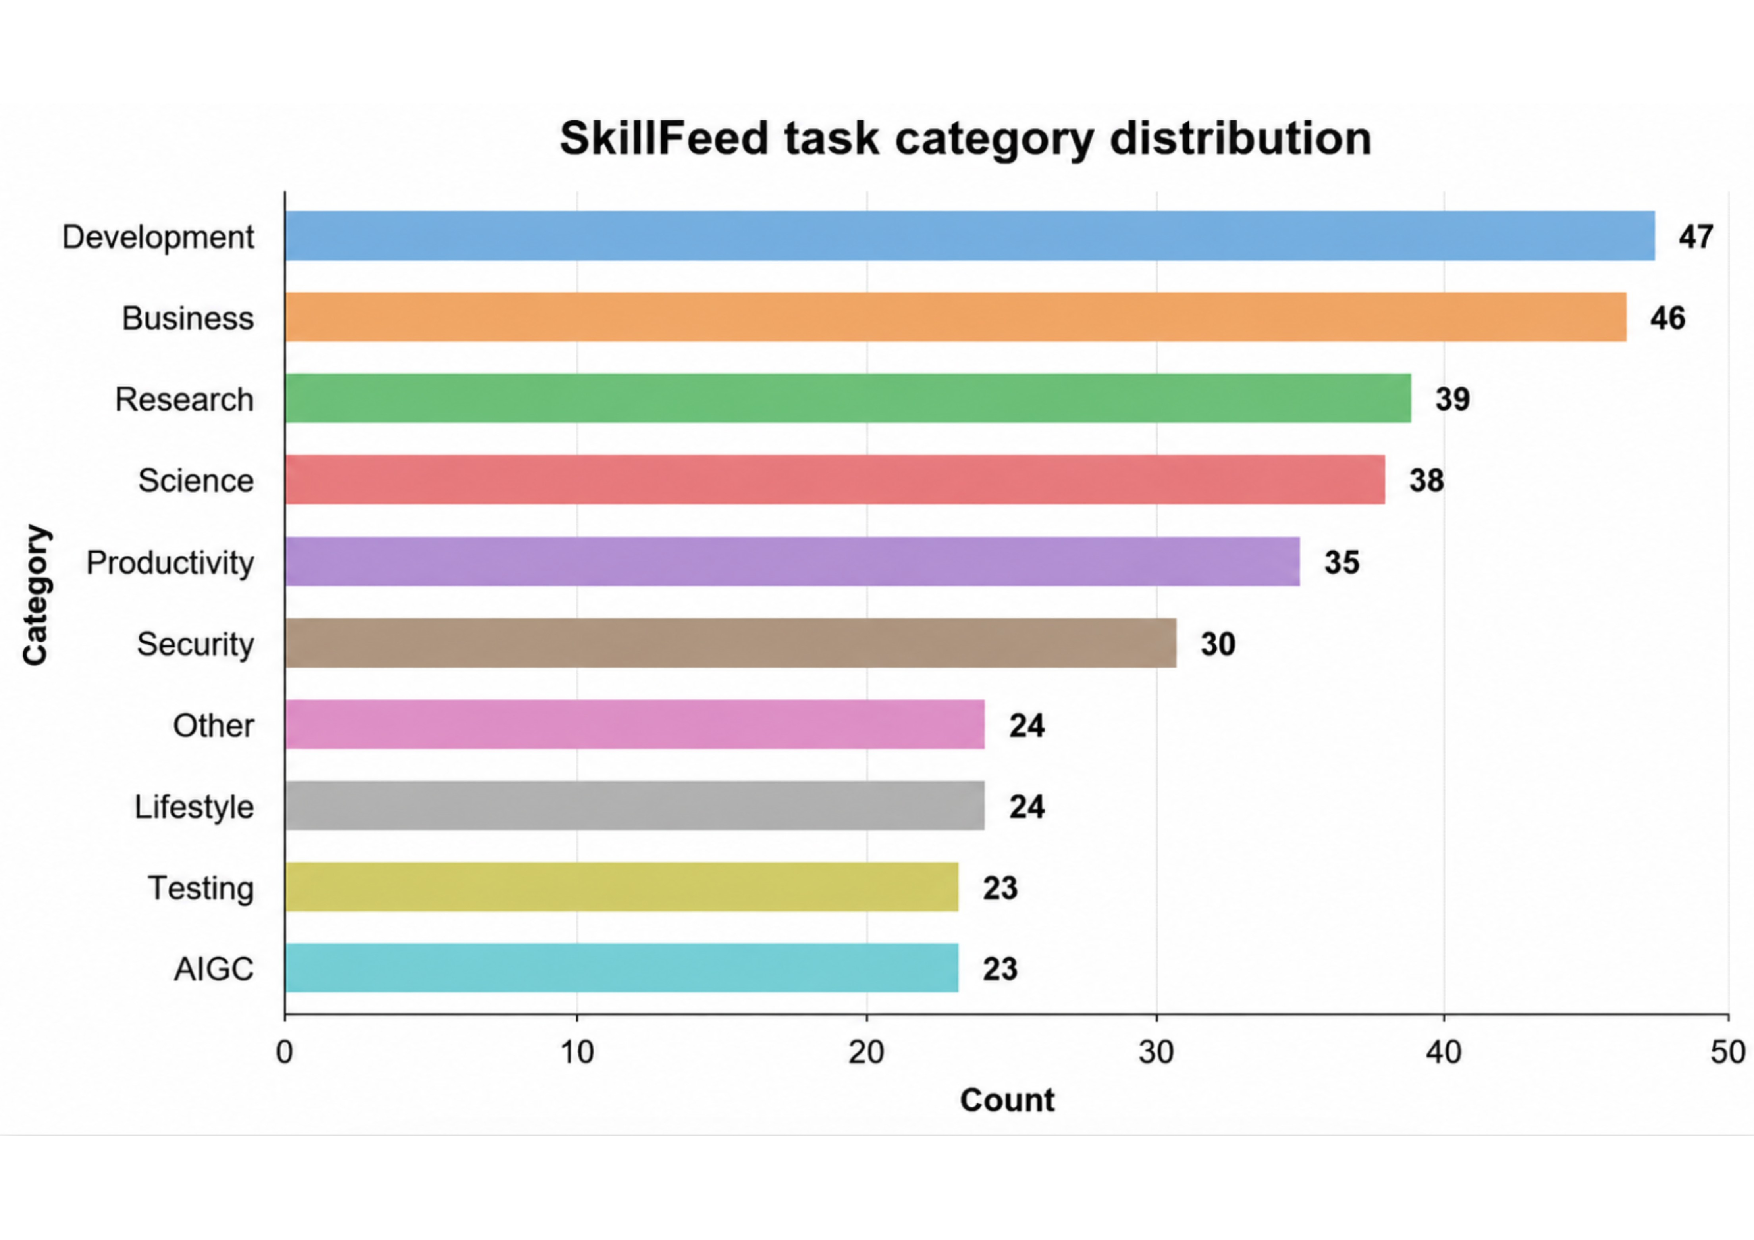
\includegraphics[width=0.8\columnwidth]{Figures/bench_distribution.pdf}
    \caption{SkillFeed-Bench consists of tasks spanning 10 categories.}
    \label{fig:category_distribution}
\end{figure}

Table~\ref{tab:dataset_stats} summarizes the key statistics. The test set consists of 329 samples drawn from a candidate pool of 228,432 skills. Each sample is annotated with 4 hard negative skills that are semantically similar but profile-incompatible. The average task description is 61.8 words, and the average skill body excerpt is 16,730 characters. To prevent trivial lexical matching, we enforce a token overlap threshold of $\leq 0.50$ between the task description and the ground-truth skill body, with an average overlap of 0.29. The annotator confidence averages 0.92, indicating high annotation quality.

\begin{table}[h]
\centering
\caption{Key statistics of SkillFeed-Bench.}
\label{tab:dataset_stats}
\begin{tabular}{l r}
\toprule
\textbf{Statistic} & \textbf{Value} \\
\midrule
Total skill candidates & 228,432 \\
Test samples & 329 \\
\quad -- Profile-sensitive & 162 \\
\quad \qquad -- Profile counterfactual & 77 \\
\quad \qquad -- Standard (with constraints) & 85 \\
\quad -- Profile-insensitive & 167 \\
Unique skill categories & 10 \\
Avg.\ task description length (words) & 61.8 \\
Avg.\ skill body excerpt length (chars) & 16,730 \\
Token overlap (task--skill body) & 0.29 (max 0.50) \\
Annotator confidence (avg.) & 0.92 \\
\bottomrule
\end{tabular}
\end{table}



The test set covers 10 skill categories spanning a diverse range of domains. As shown in Table~\ref{fig:category_distribution}, the two largest categories are Development (47 samples, 14.3\%) and Business (46 samples, 14.0\%), followed by Research (39, 11.9\%) and Science (38, 11.6\%). The remaining six categories---Productivity, Security, Other, Lifestyle, Testing, and AIGC---each contribute 23--35 samples (7.0\%--10.6\%), ensuring a balanced coverage across application domains.






\section{Training and Pipeline}
\subsection{Learning Profile-Conditioned Routing}
% \liu{I have provided a version here that can replace the subsection "User Profile-aware Retrieval Model Learning". You can further supplement and modify this version.}

\paragraph{User Profile-Aware Supervision Construction.}
% Existing skill retrieval datasets such as SkillRet\cite{cho2026skillretlargescalebenchmarkskill}, SkillsBench \cite{li2026skillsbenchbenchmarkingagentskills} SWE-Skills\cite{han2026sweskillsbenchagentskillsactually} and SRA \cite{su2026skillretrievalaugmentationagentic} are valuable for general skill retrieval, but they are insufficient for modeling personalized skill routing. To address this limitation, as illustrated in the right-hand flow of Figure~\ref{fig:benchmark}, a dataset is constructed specifically for training personalized recommendation models, incorporating both explicit persona-based supervision and counterfactual supervision.

Existing skill retrieval datasets such as SkillRet~\cite{cho2026skillretlargescalebenchmarkskill}, SkillsBench~\cite{li2026skillsbenchbenchmarkingagentskills}, SWE-Skills~\cite{han2026sweskillsbenchagentskillsactually}, and SRA~\cite{su2026skillretrievalaugmentationagentic} are valuable for general skill retrieval, but they are insufficient for modeling personalized skill routing. To address this limitation, as illustrated in the right-hand flow of Figure~\ref{fig:benchmark}, we construct a training dataset that incorporates both profile-based and counterfactual supervision.

Starting from a target skill $S^{+}$, an LLM generates a realistic task query $q$ and a compatible profile $p$ based on the skill description and procedural content. The profile captures routing-relevant constraints, such as language, region, preferred platform, and payment method. We then construct a hard-negative set $\mathcal{S}^{-}$ by combining semantic retrieval with LLM-based verification, prioritizing skills that are relevant to the task but incompatible with the user profile. This process yields task-centric supervision tuples $(p,q,S^{+},\mathcal{S}^{-})$.

To strengthen user profile-conditioned supervision, we further perform target-first counterfactual augmentation. Specifically, a hard negative $\tilde{S}^{+}\in\mathcal{S}^{-}$ is selected as the counterfactual target, and an LLM generates a new profile $\tilde{p}$ under which $\tilde{S}^{+}$ is preferred for the same query, yielding $(\tilde{p},q,\tilde{S}^{+},\tilde{\mathcal{S}}^{-})$. These paired instances provide direct supervision for learning how profile changes affect skill preference while the task remains unchanged. Finally, we filter likely valid alternatives, near-duplicate skills, and candidates without valid skill content to reduce false negatives. The resulting dataset contains 2,712 task-centric and 7,459 user profile-conditioned instances, with representative examples shown in Appendix Table~\ref{tab:training_examples_persona}.

% Training Data Examples - Final Version
\begin{table*}[t]
\centering
\small
\begin{tabular}{p{0.12\linewidth} p{0.40\linewidth} p{0.40\linewidth}}
\toprule
& \textbf{Phase 1: Task-Only Training Data} & \textbf{Phase 2: Profile-Conditioned Training Data} \\
\midrule

\textbf{Task} &
\multicolumn{2}{p{0.82\linewidth}}{
I want to plan a trip to Shanghai including attractions and a simple schedule.
}
\\

\midrule

\textbf{User Profile} &
(Not included in query)
&
Occupation: Student \\
&
&
Budget: Low budget \\
&
&
Transportation: Subway preferred
\\

\midrule

\textbf{Query Format} &
\begin{tabular}[t]{@{}p{\linewidth}@{}}
Task name: Shanghai Travel Planning\\
Task description: Plan a trip to Shanghai including attractions and a simple itinerary.\\
\end{tabular}
&
\begin{tabular}[t]{@{}p{\linewidth}@{}}
Task name: Shanghai Travel Planning\\
Task description: Plan a trip to Shanghai including attractions and a simple itinerary.\\
User/context constraints:\\
occupation: Student\\
budget: Low budget\\
transportation: Subway preferred
\end{tabular}
\\

\midrule

\textbf{Ground Truth} &
\texttt{city-travel-guide} 
&
\texttt{budget-travel-planner} 
\\

\midrule

\textbf{Why GT is correct} &
The query only specifies the travel planning task, so a general-purpose travel planning skill is sufficient.
&
The user profile indicates limited budget and preference for public transportation, making a budget-oriented planner the most suitable skill.
\\

\midrule

\textbf{Hard Negative} &
\texttt{attraction-recommender} 
&
\texttt{luxury-itinerary-planner} 

\\

\midrule

\textbf{Why HN is wrong} &
The skill focuses only on attraction recommendation and cannot generate a complete travel itinerary.
&
Assumes premium travel preferences and taxi transportation, which conflict with the user profile.
\\

\bottomrule
\end{tabular}
\caption{Training data examples for two-stage skill retrieval. Phase~1 learns general task-to-skill matching using only the task description, while Phase~2 incorporates user profile constraints to enable personalized skill selection.}
\label{tab:training_examples_persona}
\end{table*}

\paragraph{Two-Phase Retriever Training.}
Using the constructed supervision dataset, we adapt Qwen3-Embedding-0.6B and Qwen3-Reranker-0.6B~\cite{qwen3embedding} to their complementary roles in personalized skill routing. The dense retriever must preserve broad task--skill relevance while incorporating user profile information into candidate recall, whereas the reranker focuses on fine-grained user profile-conditioned discrimination among semantically relevant candidates.


% 方法 格式 设置 输入 loss

We optimize the retriever in two phases. Although the pretrained embedding model captures general semantic similarity, it is not specialized for skill routing, which requires matching task requirements to the capabilities and applicability conditions encoded in skill documents. Phase~1 therefore uses task-only queries and hard negatives to learn routing-specific task--skill alignment. Phase 2 appends profile constraints to the query and introduces paired instances in which the same task is associated with different reference skills. This schedule first adapts the model to skill routing and then learns user profile-conditioned discrimination.

For each training instance, let $u_i$ denote the query representation,
$S_i^{+}$ the reference skill, and $\mathcal{N}_i$ the set of curated
and in-batch negative skills. In Phase~1, the query contains only the task,
i.e., $u_i=q_i$. In Phase~2, the user profile is appended to the task,
i.e., $u_i=[q_i;p_i]$.

We optimize the dense retriever with the InfoNCE objective \cite{oord2019representationlearningcontrastivepredictive}:
\begin{equation}
\mathcal{L}_{\mathrm{ret}}
=
-\frac{1}{B}
\sum_{i=1}^{B}
\log
\frac{
\exp\!\left(
\operatorname{sim}
\left(
E_{\theta}(u_i),
E_{\theta}(S_i^{+})
\right)/\tau_{\mathrm{ret}}
\right)
}{
\sum\limits_{S\in\{S_i^{+}\}\cup\mathcal{N}_i}
\exp\!\left(
\operatorname{sim}
\left(
E_{\theta}(u_i),
E_{\theta}(S)
\right)/\tau_{\mathrm{ret}}
\right)
},
\label{eq:app_retriever_loss}
\end{equation}
where $E_{\theta}$ is the dense encoder,
$\operatorname{sim}(\cdot,\cdot)$ denotes cosine similarity,
$B$ is the batch size, and $\tau_{\mathrm{ret}}$ is the temperature.
The objective encourages the reference skill to be ranked above skills that
are task-relevant but incompatible with the user profile.

% We adopt a two-phase optimization strategy for the dense retriever. Directly training on persona-conditioned queries risks the model
% overfitting to explicit persona attributes while underlearning the fundamental task--skill semantic
% relationships that form the basis of effective retrieval. A progressive training schedule mitigates this by first establishing strong
% semantic alignment and then layering persona-aware discrimination on top.

% In the first phase, the retriever is trained with task-only queries containing no persona information. Each query presents the task name,
% description, and core requirements, paired with the ground-truth skill as the positive document and embedding-based hard negatives. This
% teaches the model to match tasks to skills based on functional relevance alone. In the second phase, persona constraints—country, language,
% domain, and other user-context factors—are a\%ended to the query. The training data is augmented with persona counterfactual samples: for
% the same task, different persona specifications yield different ground-truth skills, and these become mutual negatives. This teaches the
% retriever that persona can flip the correct skill for an otherwise identical task.

% This two-phase a\%roach yields a retriever that retains strong semantic matching while gaining personalization sensitivity.with the gain concentrated on
% persona-sensitive queries where context-dependent skill disambiguation is required.

% Each training instance contains one positive skill and multiple hard negatives mined from the skill repository. Since these negatives are semantically similar to the target skill and often differ only in persona compatibility, retrieval naturally becomes a contrastive ranking problem. We therefore optimize the retriever using the InfoNCE objective:

% % \begin{equation}
% % \mathcal{L}_{\text{InfoNCE}}
% % =
% % -
% % \log
% % \frac{
% % \exp(\mathrm{sim}(q,s^{+})/\tau)
% % }
% % {
% % \exp(\mathrm{sim}(q,s^{+})/\tau)
% % +
% % \sum_{j=1}^{K}
% % \exp(\mathrm{sim}(q,s_j^{-})/\tau)
% % },
% % \end{equation}

% \begin{equation}
% \mathcal{L}_{\text{InfoNCE}}
% =
% -\log
% \frac{
% \exp(\mathrm{sim}(q,s^{+})/\tau)
% }{
% \sum\limits_{s\in\{s^{+}\}\cup\mathcal{N}}
% \exp(\mathrm{sim}(q,s)/\tau)
% },
% \end{equation}

% where $s^{+}$ denotes the positive skill, $\mathcal{N}$ denotes the set of hard negative skills mined for the query, $\mathrm{sim}(\cdot,\cdot)$ represents cosine similarity between query and skill embeddings, and $\tau$ is a temperature parameter.

% We fine-tune the retriever end-to-end on 2$\times$A100 GPUs with per-device batch size 1 and gradient accumulation over 16 steps, yielding
% an effective batch of 16 query--candidate groups per update. Training runs for 3 epochs with a maximum sequence length of 2048 under
% DeepSpeed ZeRO-2.

\paragraph{Persona-Aware Reranker Training.}
Unlike the dense retriever, the reranker is trained directly with user profile-aware supervision because it operates on a small candidate set whose members are already relevant to the task. Its primary role is therefore to determine which candidate best satisfies the user profile-specific constraints. For each query containing both task and profile information, we construct a ranking group consisting of one positive skill and multiple curated hard negatives. Each candidate is represented by its name, description, and procedural body.


The reranker operates on a candidate group containing one reference skill
$S_i^{+}$ and a set of hard negatives $\mathcal{N}_i$. Given query $u_i$
and candidate skill $S$, Qwen3-Reranker produces a relevance score
$r_{\phi}(u_i,S)$ from the logit assigned to the token \textit{yes}.
We optimize the model using listwise cross-entropy:
\begin{equation}
\mathcal{L}_{\mathrm{rank}}
=
-\frac{1}{B}
\sum_{i=1}^{B}
\log
\frac{
\exp\!\left(
r_{\phi}(u_i,S_i^{+})/\tau_{\mathrm{rank}}
\right)
}{
\sum\limits_{S\in\{S_i^{+}\}\cup\mathcal{N}_i}
\exp\!\left(
r_{\phi}(u_i,S)/\tau_{\mathrm{rank}}
\right)
},
\label{eq:app_reranker_loss}
\end{equation}
where $\tau_{\mathrm{rank}}$ is the ranking temperature. Normalizing scores
within each candidate group directly trains the reference skill to outrank
semantically similar alternatives.

% We employ Qwen3-Reranker as a generative relevance judge. Given an instruction, a query, and a candidate skill, the model assesses whether the candidate satisfies the query, and its logit for the token \textit{yes} is used as the relevance score $r_{\phi}(u,S)$. The reranker is optimized with a listwise objective \cite{10.1145/1390156.1390306}:
% \begin{equation}
% \mathcal{L}_{\mathrm{rank}}
% =
% -\frac{1}{B}
% \sum_{i=1}^{B}
% \log
% \frac{
% \exp\!\left(
% r_{\phi}(u_i,S_i^{+})/\tau_{\mathrm{rank}}
% \right)
% }{
% \sum\limits_{S\in\{S_i^{+}\}\cup\mathcal{N}_i}
% \exp\!\left(
% r_{\phi}(u_i,S)/\tau_{\mathrm{rank}}
% \right)
% },
% \end{equation}
% where $\tau_{\mathrm{rank}}$ is the ranking temperature. By normalizing scores within each candidate group, the objective directly encourages the user profile-compatible target skill to outrank semantically similar alternatives.



% Unlike the retriever, the reranker operates on a small candidate set that is already semantically relevant to the task. Its role is therefore not broad semantic matching but final persona-conditioned discrimination. Given a query containing the task and persona constraints, we form a ranking group from the retriever outputs with one positive skill and multiple hard negatives. 

% As a result, personalized skill recommendation naturally becomes a relative ranking problem rather than an independent binary classification problem. We therefore adopt a listwise ranking objective:
% \begin{equation}
% \mathcal{L}_{\text{rank}}
% =
% -
% \log
% \frac{
% \exp(r^{+}/\tau)
% }
% {
% \sum_{i=1}^{N}
% \exp(r_i/\tau)
% },
% \end{equation}
% where $r^{+}$ denotes the relevance score assigned to the target skill, $\{r_i\}_{i=1}^{N}$ are the scores of all candidates within the ranking group, and $\tau$ is a temperature parameter.

% We fine-tune the reranker on 1$\times$A100 with batch size 4 and gradient accumulation over 4 steps, matching the same effective
% batch size of 16. Training runs for 3 epochs with a cosine learning rate schedule and 10\% warmup.




% \subsection{Persona-aware Retrieval Model Learning} % v1
% % 为什么训练embedding 和 reranker模型是必要的 因为现有的模型只能基于语义匹配但是忽视用户信息 然后我们使用上一章得到的训练数据 基于Qwen3-Embedding-0.6B 和Qwen3-Reranker-0.6B进行了微调 然后再在两个subsection分别写怎么微调的 见training detail文档

% Existing retrieval models are primarily trained for task--skill semantic matching and therefore cannot effectively distinguish skills that are semantically similar but suitable for different user personas. Using the supervision dataset constructed in \ref{subsection:Persona-aware Supervision Construction} section, we fine-tune Qwen3-Embedding-0.6B and Qwen3-Reranker-0.6B \cite{qwen3embedding} to learn persona-aware retrieval and ranking behaviors.


% % 方法 格式 设置 输入 loss
% \subsubsection{Dense Retriever Adaptation}
% We adopt a two-phase optimization strategy for the dense retriever. Directly training on persona-conditioned queries may bias the model toward explicit persona signals while weakening the learning of fundamental task--skill semantic associations. A progressive training schedule alleviates this issue by first establishing robust semantic alignment and subsequently incorporating persona-aware discrimination.

% In the first phase, the retriever is trained with task-only queries—task name, description, and core requirements—paired with ground-truth
% skills and embedding-based hard negatives, learning to match tasks to skills based on functional relevance alone. In the second phase,
% persona constraints are appended to the query. The training data is augmented
% with persona counterfactual samples, where different persona specifications yield different ground-truth skills for the same task; these
% become mutual negatives, teaching the retriever that persona can flip the correct skill for an otherwise identical task.

% This two-phase approach yields a retriever that retains strong semantic matching while gaining personalization sensitivity, with the gain
% concentrated on persona-sensitive queries where context-dependent skill disambiguation is required.
% % We adopt a two-phase optimization strategy for the dense retriever. Directly training on persona-conditioned queries risks the model
% % overfitting to explicit persona attributes while underlearning the fundamental task--skill semantic
% % relationships that form the basis of effective retrieval. A progressive training schedule mitigates this by first establishing strong
% % semantic alignment and then layering persona-aware discrimination on top.

% % In the first phase, the retriever is trained with task-only queries containing no persona information. Each query presents the task name,
% % description, and core requirements, paired with the ground-truth skill as the positive document and embedding-based hard negatives. This
% % teaches the model to match tasks to skills based on functional relevance alone. In the second phase, persona constraints—country, language,
% % domain, and other user-context factors—are a\%ended to the query. The training data is augmented with persona counterfactual samples: for
% % the same task, different persona specifications yield different ground-truth skills, and these become mutual negatives. This teaches the
% % retriever that persona can flip the correct skill for an otherwise identical task.

% % This two-phase a\%roach yields a retriever that retains strong semantic matching while gaining personalization sensitivity.with the gain concentrated on
% % persona-sensitive queries where context-dependent skill disambiguation is required.

% Each training instance contains one positive skill and multiple hard negatives mined from the skill repository. Since these negatives are semantically similar to the target skill and often differ only in persona compatibility, retrieval naturally becomes a contrastive ranking problem. We therefore optimize the retriever using the InfoNCE objective:

% % \begin{equation}
% % \mathcal{L}_{\text{InfoNCE}}
% % =
% % -
% % \log
% % \frac{
% % \exp(\mathrm{sim}(q,s^{+})/\tau)
% % }
% % {
% % \exp(\mathrm{sim}(q,s^{+})/\tau)
% % +
% % \sum_{j=1}^{K}
% % \exp(\mathrm{sim}(q,s_j^{-})/\tau)
% % },
% % \end{equation}

% \begin{equation}
% \mathcal{L}_{\text{InfoNCE}}
% =
% -\log
% \frac{
% \exp(\mathrm{sim}(q,s^{+})/\tau)
% }{
% \sum\limits_{s\in\{s^{+}\}\cup\mathcal{N}}
% \exp(\mathrm{sim}(q,s)/\tau)
% },
% \end{equation}

% where $s^{+}$ denotes the positive skill, $\mathcal{N}$ denotes the set of hard negative skills mined for the query, $\mathrm{sim}(\cdot,\cdot)$ represents cosine similarity between query and skill embeddings, and $\tau$ is a temperature parameter.

% % We fine-tune the retriever end-to-end on 2$\times$A100 GPUs with per-device batch size 1 and gradient accumulation over 16 steps, yielding
% % an effective batch of 16 query--candidate groups per update. Training runs for 3 epochs with a maximum sequence length of 2048 under
% % DeepSpeed ZeRO-2.
  
% \subsubsection{Generative Reranker Adaptation}
% %  reranker 只有一阶段 先解释和embedding的差异 所以只需要一阶段训练 然后介绍训练方法

% % Unlike the dense retriever, the reranker is directly optimized using the final persona-aware supervision constructed in Section~4.1. This
% % design is motivated by the different roles of the two components. The retriever operates over the entire skill repository and must first
% % establish robust task--skill semantic alignment before learning persona-dependent preferences. In contrast, the reranker only processes a
% % small set of candidates that have already been filtered by the retriever and are therefore highly relevant to the task. The primary
% % challenge at this stage is no longer semantic matching, but distinguishing candidates according to persona-specific constraints.
% % Consequently, directly training the reranker on persona-aware supervision is sufficient and more effective.

% Unlike the dense retriever, the reranker is directly trained with persona-aware supervision. This is because its input
%   candidates are already semantically relevant to the task—the challenge shifts from semantic matching to persona-based disambiguation.

% % For each query, we first retrieve the top-$K$ candidate skills using the trained dense retriever and construct a ranking group containing
% % one positive skill and multiple hard negatives. The query includes both task information and persona constraints, while each candidate skill
% % is represented by its name, description, and skill body. The reranker scores each candidate by computing the log-likelihood of a positive
% % judgment given the query--candidate pair, enabling fine-grained modeling of how well each skill satisfies both the task requirements and the
% % user context.
% Given a query containing both task and persona constraints, we retrieve the top-$K$ candidates from the trained retriever and form a ranking
% group of one positive and multiple hard negatives. 

% As a result, personalized skill recommendation naturally becomes a relative ranking problem rather than an independent binary classification problem. We therefore adopt a listwise ranking objective:
% \begin{equation}
% \mathcal{L}_{\text{rank}}
% =
% -
% \log
% \frac{
% \exp(r^{+}/\tau)
% }
% {
% \sum_{i=1}^{N}
% \exp(r_i/\tau)
% },
% \end{equation}
% where $r^{+}$ denotes the relevance score assigned to the target skill, $\{r_i\}_{i=1}^{N}$ are the scores of all candidates within the ranking group, and $\tau$ is a temperature parameter.

% % We fine-tune the reranker on 1$\times$A100 with batch size 4 and gradient accumulation over 4 steps, matching the same effective
% % batch size of 16. Training runs for 3 epochs with a cosine learning rate schedule and 10\% warmup.


% Both models are fine-tuned end-to-end on 2$\times$A100 GPUs with AdamW ($\text{lr}=1\times10^{-5}$), effective batch size
% 16, and a maximum sequence length of 2048 over 3 epochs. 

\subsection{Persona-Aware Routing Pipeline}
\label{subsection:two_stage_inference}

At inference time, SkillFeed adopts a two-stage inference pipeline that separates broad candidate coverage from fine-grained candidate discrimination.
The first stage retrieves candidate skills from the 228K-scale repository, and the second stage reranks the retrieved candidates.
This separation allows the recall stage to focus on preserving potentially relevant skills, while the reranker determines which candidate best satisfies both the task requirement and the user profile.

% \liu{The "\texttt{SKILL. md} Chunk Index" section is a bit verbose, so merge it into the Candidate Recall paragraph}
\paragraph{Candidate Recall.}
The recall stage combines three complementary retrieval channels.
The first channel is task-oriented dense retrieval, which encodes the task name and task description as the query and retrieves skills according to their names and descriptions.
The second channel applies BM25 over the same skill-level text, providing a lexical matching signal complementary to dense retrieval~\citep{robertson2009bm25}.
The third channel is persona-conditioned dense retrieval over structured chunks extracted from \texttt{SKILL.md} bodies.
Unlike the first two channels, which rely on skill-level summaries, this channel exposes body-level evidence during recall and is designed to capture fine-grained user profile-related information.

% \paragraph{\texttt{SKILL.md} Chunk Index.}
Skill descriptions are usually concise and mainly summarize the core function of a skill \cite{openai2026skills}.
However, whether a skill is suitable for a particular user often depends on details that may appear only in the skill body, such as applicable scenarios, input requirements, output formats, tool dependencies, constraints, and examples.
These details are commonly distributed across sections such as \textit{When to use}, \textit{Inputs}, \textit{Examples}, \textit{Constraints}, and \textit{Dependencies}.
Therefore, relying only on skill names and descriptions may miss candidates whose main function is relevant but whose user profile-specific applicability is expressed in the body text.

\paragraph{Skill-to-Chunk Representation.}
A straightforward alternative is to embed the entire \texttt{SKILL.md} file as a single document.
However, this may produce overly coarse representations, since long-document embeddings tend to mix multiple capabilities, conditions, and constraints.
As a result, localized but important matching signals may be diluted.
Following passage-level retrieval in retrieval-augmented generation~\citep{lewis2020rag}, we instead split each \texttt{SKILL.md} file into Markdown-structured chunks and encode these shorter passages independently.

% For each chunk, we preserve its skill identity and section path:
% \[
% \begin{aligned}
% &\texttt{Skill: name}\\
% &\texttt{Description: description}\\
% &\texttt{Section: path}\\
% &\texttt{Content: chunk}.
% \end{aligned}
% \]

For each chunk, we store the skill name, description, section path, and content.
Long sections are further divided into overlapping passages, so that local applicability conditions can be recovered during recall.
This chunk-level index enables profile-conditioned retrieval to match user preferences and constraints against specific skill-body evidence, rather than only against high-level skill summaries.

\paragraph{Chunk-to-Skill Aggregation.}
User profile-conditioned retrieval returns chunk-level results, which are then aggregated into skill-level candidates before fusion.
For each candidate skill $S_i$, let $\mathcal{C}_{S_i}$ denote the set of
retrieved chunks belonging to $S_i$, and let $h_c$ denote the dense similarity
score of chunk $c$.
Let $\operatorname{TopM}(\mathcal{C}_{S_i})$ denote the set of the $M$
highest-scoring chunks in $\mathcal{C}_{S_i}$. The aggregated score is
computed as
\begin{equation}
\begin{aligned}
\operatorname{score}(S_i)
={}&
\alpha
\max_{c\in\mathcal{C}_{S_i}} h_c
+
\frac{\beta}{M}
\sum_{c\in\operatorname{TopM}(\mathcal{C}_{S_i})} h_c \\
&+
\gamma
\log\!\left(1+\left|\mathcal{C}_{S_i}\right|\right),
\end{aligned}
\label{eq:chunk_to_skill_aggregation}
\end{equation}
where $\alpha$, $\beta$, and $\gamma$ are non-negative aggregation weights,
and $M$ is the number of highest-scoring chunks included in the mean
term. The maximum term captures the strongest local match between the user profile and a passage in the skill body. 
The top-$M$ mean term measures whether the skill is supported by multiple highly relevant chunks, thereby reducing the influence of an isolated noisy match. 
The logarithmic count term provides a mild reward for skills associated with multiple retrieved chunks.
Overall, this aggregation favors skills with consistent body-level evidence while preventing an excessive preference for skills containing a larger
number of chunks.

\paragraph{Fusion and Profile-Aware Reranking.}
The three recall lists are combined using weighted reciprocal rank fusion~\citep{cormack2009rrf}.
The fused top candidates are then passed to the trained reranker, which takes the task, the user profile, and the full candidate skill information as input.
In this pipeline, chunk-based retrieval is used to improve user profile-aware candidate coverage during recall.
It does not directly determine the final ranking; instead, it increases the likelihood that skills with relevant body-level evidence are included for subsequent fine-grained reranking.



\section{Additional Experimental Details}
\label{app:experimental_details}

\subsection{Dataset Structure and Input Formatting}
\label{app:dataset_format}

\paragraph{Underlying Sample Schema.}
Each source instance contains a task, an optional user profile, one reference
skill, and a set of hard-negative skills:
\begin{appendixcode}
{
  "task": {
    "name": "...",
    "description": "...",
    "core_requirements": ["...", "..."]
  },
  "user_context_constraints": {
    "country_region": "...",
    "language": "...",
    "preferred_platforms": ["..."],
    "payment_methods": ["..."],
    "other_constraints": ["..."]
  },
  "ground_truth_skill": {...},
  "hard_negative_skills": [{...}, {...}]
}
\end{appendixcode}

Each skill record contains a name, description, and a
\texttt{SKILL.md} body excerpt. The reference skill is treated as the
single annotated positive for training and evaluation.

\paragraph{Phase 1: Task-Only Supervision.}
Phase~1 removes the user profile from the query and uses task-centric
supervision. The query instruction is:
\begin{quote}
\small
\texttt{Represent this user task for retrieving the most appropriate skill.}
\end{quote}
The resulting query is formatted as:
\begin{appendixcode}
Represent this user task for retrieving the most appropriate skill.

Task name: {task_name}

Task description: {task_description}

Core requirements:
- {requirement_1}
- {requirement_2}
\end{appendixcode}
The training record follows the ms-swift embedding schema:
\begin{appendixcode}
{
  "messages": [{"role": "user", "content": "<query>"}],
  "positive_messages": [
    [{"role": "user", "content": "<positive_skill>"}]
  ],
  "negative_messages": [
    [{"role": "user", "content": "<negative_skill_1>"}],
    [{"role": "user", "content": "<negative_skill_2>"}]
  ]
}
\end{appendixcode}

Phase~1 contains 2,712 training instances and 356 validation instances.

\paragraph{Phase 2: Profile-Conditioned Supervision.}
Phase~2 retains the same task fields and appends user-context constraints:
\begin{appendixcode}
Represent this user task for retrieving the most appropriate skill.

Task name: {task_name}

Task description: {task_description}

Core requirements:
- {requirement_1}
- {requirement_2}

User/context constraints:
country_region: {region}
language: {language}
preferred_platforms: {platforms}
payment_methods: {payment_methods}
other_constraints: {constraints}
\end{appendixcode}

Its negatives combine curated hard negatives, LLM-guided
profile-conflicting negatives, and counterfactual positives from other
profile variants of the same task. The Phase~2 corpus contains 7,459
training instances and 608 validation instances, including full-body and
profile-counterfactual supervision.

\paragraph{Skill Document Format.}
Positive and negative skills are serialized with the same field order:
\begin{appendixcode}
Skill name: {skill_name}

Skill description: {skill_description}

Skill body:
{skill_body_excerpt}
\end{appendixcode}
The body excerpt exposes procedural details and applicability constraints
that are not always present in the short description.

\paragraph{Reranker Records.}
Reranker training uses the task--profile query together with a candidate
group containing one positive and multiple negatives. The generative
reranker record is:
\begin{appendixcode}
{
  "system":
    "Judge whether the Document meets the requirements based
     on the Query and the Instruct provided. Note that the
     answer can only be \"yes\" or \"no\".",
  "messages": [{"role": "user", "content": "<query>"}],
  "positive_messages": [
    [{"role": "assistant", "content": "<positive_skill>"}]
  ],
  "negative_messages": [
    [{"role": "assistant", "content": "<negative_skill_1>"}],
    [{"role": "assistant", "content": "<negative_skill_2>"}]
  ]
}
\end{appendixcode}

The document role is \texttt{user} for embedding records and
\texttt{assistant} for generative reranker records. During reranker
training and inference, the system instruction, query template, skill field
names, and constraint serialization are kept consistent to avoid formatting
artifacts.


\subsection{Training Objectives}
\label{app:training_objectives}



\subsection{Implementation Details}
\label{app:implementation_details}

The SkillFeed dense retriever is initialized from
Qwen3-Embedding-0.6B, and the SkillFeed reranker is initialized from
Qwen3-Reranker-0.6B. Both models are fine-tuned on 2$\times$A100 GPUs using
AdamW with a learning rate of $1\times10^{-5}$, an effective batch size of 16,
a maximum sequence length of 2048, and three training epochs. The retriever is
trained in two phases: 2,712 task-centric instances are used for task-only
alignment, followed by 7,459 user profile-conditioned instances for
profile-aware adaptation. Lexical-overlap filtering uses a threshold of 0.50.

For \texttt{SKILL.md} chunk retrieval, Markdown sections are divided into
passages with a target length of 200--500 tokens, a maximum length of 800
tokens, and a small overlap between adjacent passages. Chunk-to-skill
aggregation uses $\alpha=0.70$, $\beta=0.25$, $\gamma=0.05$, and $M=3$.
Weighted reciprocal rank fusion assigns weights of 0.40 to task dense
retrieval, 0.40 to profile-conditioned dense retrieval over
\texttt{SKILL.md} chunks, and 0.20 to BM25. Unless otherwise stated, the full
pipeline reranks the top 50 fused candidates; the top-100 setting is evaluated
only in the ablation study.



% Persona Analysis - Combined Table (Exp 2: Phase 2 + Our FT Reranker with Persona)
% Uses ALL 329 samples (including those with rank > 50)
\begin{table}[!htbp]
\centering
\caption[Per-Profile-group analysis]{Per-Profile-group analysis on SkillFeed Emb Phase 2 + SkillFeed Reranker with Profile. We evaluate performance across different persona groups: country/region, language, domain, and persona sensitivity. All 329 test samples are included.}
\label{tab:persona_analysis}
% \resizebox{\columnwidth}{!}{%
\begin{tabular}{l c c c c c}
\toprule
\textbf{Group} & \textbf{N} & \textbf{Hit@1} & \textbf{Hit@5} & \textbf{MRR@20} & \textbf{nDCG@20} \\
\midrule
\multicolumn{6}{l}{\textit{By Country/Region}} \\
Global/Unknown & 257 & 0.735 & 0.879 & 0.795 & 0.827 \\
United States & 46 & 0.717 & 0.804 & 0.760 & 0.785 \\
China & 14 & 0.571 & 0.714 & 0.648 & 0.696 \\
Other Regions & 12 & 0.917 & 0.917 & 0.917 & 0.917 \\
\midrule
\multicolumn{6}{l}{\textit{By Language}} \\
English & 204 & 0.672 & 0.804 & 0.735 & 0.770 \\
Unknown & 100 & 0.870 & 0.980 & 0.907 & 0.927 \\
Programming & 11 & 0.545 & 0.818 & 0.632 & 0.677 \\
Other Languages & 14 & 0.786 & 0.929 & 0.845 & 0.866 \\
\midrule
\multicolumn{6}{l}{\textit{By Domain}} \\
General & 248 & 0.790 & 0.895 & 0.836 & 0.860 \\
Tech & 44 & 0.614 & 0.818 & 0.692 & 0.738 \\
Science & 15 & 0.533 & 0.800 & 0.663 & 0.727 \\
Other Domains & 22 & 0.455 & 0.682 & 0.530 & 0.577 \\
% \midrule
% \multicolumn{6}{l}{\textit{By Persona Sensitivity}} \\
% Persona-Insensitive & 167 & 0.832 & 0.928 & 0.873 & 0.892 \\
% Persona-Sensitive & 162 & 0.630 & 0.796 & 0.701 & 0.743 \\
\midrule
\multicolumn{6}{l}{\textit{Overall}} \\
\textbf{Overall} & \textbf{329} & \textbf{0.733} & \textbf{0.863} & \textbf{0.788} & \textbf{0.819} \\
\bottomrule
\end{tabular}%
% }
\end{table}

% \paragraph{Persona information.}
% Table~\ref{tab:ablation_persona} isolates the effect of persona at each stage. Incorporating persona in the embedding yields +13.4\% (Phase~1: 0.483 $\rightarrow$ Phase~2:
% 0.617), while adding persona to the reranker yields +8.9\% (0.644 $\rightarrow$ 0.733). The combined effect is largely additive, indicating that persona information operates
% orthogonally at the retrieval and reranking stages.



% Statistical Significance Analysis
\begin{table}[!htbp]
\centering
\caption{Bootstrap 95\% confidence intervals for key configurations.}
\label{tab:bootstrap_ci}
% \resizebox{\columnwidth}{!}{%
\begin{tabular}{l c c c c}
\toprule
\textbf{Configuration} & \textbf{Hit@1} & \textbf{95\% CI} & \textbf{MRR@20} & \textbf{95\% CI} \\
\midrule
Full Pipeline & 0.751 & [0.706, 0.794] & 0.803 & [0.760, 0.846] \\
SkillFeed Emb Phase 2 + SkillFeed Reranker w Profile & 0.733 & [0.684, 0.778] & 0.788 & [0.744, 0.832] \\
SkillFeed Emb Phase 2 + SkillFeed Reranker w/o Profile & 0.644 & [0.596, 0.696] & 0.712 & [0.663, 0.761] \\
SkillFeed Emb Phase 2  & 0.617 & [0.568, 0.669] & 0.697 & [0.647, 0.746] \\
SkillFeed Emb Phase 1 & 0.483 & [0.429, 0.535] & 0.583 & [0.530, 0.636] \\
\bottomrule
\end{tabular}%
% }
\end{table}

\begin{table}[!htbp]
\centering
\caption[Permutation test results for key comparisons.]{
Permutation test results for key comparisons.
Statistical significance: $^{*}p<0.05$, $^{**}p<0.01$, and $^{***}p<0.001$.
}
\label{tab:permutation_test}
% % \resizebox{\columnwidth}{!}{%
\begin{tabular}{l c c c}
\toprule
\textbf{Comparison}
& \textbf{Hit@1 $\Delta$}
& \textbf{$p$-value}
& \textbf{Sig.} \\
\midrule

Full Pipeline vs Qwen3-Emb-0.6B + Qwen3-Reranker-0.6B
& +0.231 & $<0.0001$ & $^{***}$ \\

Embedding Only vs Embedding + SkillFeed Reranker
& +0.116 & 0.001 & $^{***}$ \\

Reranker without vs with Profile
& +0.089 & $<0.01$ & $^{**}$ \\

\bottomrule
\end{tabular}%
% }
\end{table}
% Check whether the conference requires a reproducibility checklist to be included in the paper.
% If so, you can uncomment the following line and ajust the path to include it.
% \input{ReproducibilityChecklist.tex}

\end{document}
